\def\VERSION{0.9.1.4}


\documentclass[12pt]{report}
\ProvidesPackage{musereum}
\usepackage{framed}
\usepackage{float}
\usepackage{eurosym}
\usepackage{graphicx}
\graphicspath{ {images/} }
\usepackage[T1]{fontenc}
\usepackage{titlesec, blindtext, color}
\definecolor{gray75}{gray}{0.75}
\newcommand{\hsp}{\hspace{20pt}}
\titleformat{\chapter}[hang]{\Huge\bfseries}{\thechapter\hsp\textcolor{gray75}{|}\hsp}{0pt}{\Huge\bfseries}
\titlespacing*{\chapter}{0pt}{-35pt}{40pt}

\usepackage{amsmath}
\usepackage{amsfonts}
\usepackage{amssymb}
\usepackage{booktabs}
\usepackage{pgfplots}
\usepgfplotslibrary{fillbetween}
\usepackage{multirow}

\usepackage{tikz}
\usetikzlibrary{calc,trees,positioning,arrows,chains,fit,shapes.geometric,%
    decorations.pathreplacing,decorations.pathmorphing,shapes,%
    decorations.markings,%	
    matrix,shapes.symbols}


\usepackage{amsmath}
\usepackage{graphicx}
\usepackage{hyperref}
%\hypersetup{
%    colorlinks=true,
%    linkcolor=blue,
%    filecolor=magenta,      
%    urlcolor=cyan,
%}
%Russian-specific packages
%--------------------------------------
\usepackage[T2A]{fontenc}
\usepackage[utf8]{inputenc}
%\usepackage[russian]{babel}
%--------------------------------------
 
%Hyphenation rules
%--------------------------------------
\usepackage{hyphenat}
%\hyphenation{ма-те-ма-ти-ка вос-ста-нав-ли-вать}
%--------------------------------------

\usepackage{multicol}
\setlength{\columnsep}{1.2cm}

\newcommand{\hlc}[1]{\colorbox{white!25}{#1}}

\usepackage[a4paper, total={6.5in, 8.7in}]{geometry}

\tikzstyle{event} = [trapezium, trapezium left angle=70, trapezium right angle=110, minimum width=3cm, minimum height=1cm, text centered, draw=black]
\tikzstyle{inout} = [rectangle, rounded corners, minimum width=3cm, minimum height=1cm,text centered, draw=black]
\tikzstyle{rect} = [rectangle, minimum width=3cm, minimum height=1cm, text centered, draw=black]
\tikzstyle{check} = [diamond, minimum width=3cm, minimum height=1cm, text centered, draw=black]
\tikzstyle{arrow} = [thick,->,>=stealth]
\tikzstyle{line} = [thick]
\tikzstyle{vecArrow} = [thick, decoration={markings,mark=at position
   1 with {\arrow[semithick]{open triangle 60}}},
   double distance=1.4pt, shorten >= 5.5pt,
   preaction = {decorate},
   postaction = {draw,line width=1.4pt, white,shorten >= 4.5pt}]
\tikzstyle{innerWhite} = [semithick, white,line width=1.4pt, shorten >= 4.5pt]
\pgfplotsset{
	axisPlot/.style={
	    scaled ticks=false,
		ymajorgrids=true,
		xmajorgrids=false,
		ylabel near ticks,
		xlabel near ticks,
		width=13cm,
		height=7.5cm,
	    legend cell align={left},
		legend style={at={(0,-0.20)}, anchor=north west, draw=none}
	}
}

\pgfdeclarelayer{background}
\pgfdeclarelayer{foreground}
\pgfsetlayers{background,main,foreground}

%\usepackage{musereum}
\usepackage{import}

\setlength{\parindent}{0em}
\setlength{\parskip}{0.65em}
\renewcommand{\baselinestretch}{1.1}

\definecolor{light-gray}{gray}{0.95}
\def\code#1{\colorbox{light-gray}{\texttt{#1}}}

\title{Musereum}
\author{Artem Aler Dan}
\date{\today}

\begin{document}
\begin{titlepage}
	\centering
	
	\scshape % Use small caps for all text on the title page
	\vspace*{\baselineskip} % White space at the top of the page
	
	\rule{\textwidth}{1.6pt}\vspace*{-\baselineskip}\vspace*{2pt} % Thick horizontal rule
	\rule{\textwidth}{0.4pt} % Thin horizontal rule
	
	\vspace{0.75\baselineskip} % Whitespace above the title
	
	{\Huge\textbf{MUSEREUM}} % Title
%	\vspace{0.2\baselineskip} % Whitespace below the title
	
	\rule{\textwidth}{0.4pt}\vspace*{-\baselineskip}\vspace{3.2pt} % Thin horizontal rule
	\rule{\textwidth}{1.6pt} % Thick horizontal rule
	
	\vspace{1.5\baselineskip} % Whitespace after the title block
	
	%------------------------------------------------
	%	Subtitle
	%------------------------------------------------
	
	Official Whitepaper % Subtitle or further description
	
	\small{ver.\VERSION}
	
	\vspace*{3.5\baselineskip} % Whitespace under the subtitle
	
	
	%------------------------------------------------
	%	Editor(s)
	%------------------------------------------------
	
	Edited By
	
	\vspace{0.5\baselineskip} % Whitespace before the editors
	
	{\scshape\Large Artem Abaev \\ Dan Reitman \\ Aler Denisov \\ Gleb Cohen \\} % Editor list
	
	% \vspace{0.5\baselineskip} % Whitespace below the editor list
	
	% \textit{The University of California \\ Berkeley} % Editor affiliation
	
	\vfill % Whitespace between editor names and publisher logo
	
	%------------------------------------------------
	%	Publisher
	%------------------------------------------------
		
	\vspace{0.3\baselineskip} % Whitespace under the publisher logo
	
	2017 % Publication year
	
	{\large Musereum Team} % Publisher

\end{titlepage}
%\maketitle
\pagebreak
\tableofcontents
\pagebreak

\chapter{Introduction}
\label{overview}
%\begin{multicols}{2}
Musereum is a blockchain-based project created by a consortium of blockchain professionals together with software development experts, lawyers and professional members of music industry. The expertise of the developing members allows for implementation of mentioned industries and technology to cope with realistic business challenges and transform the transactional structure of the global music industry.

The project represents a music platform based on smart contracts. Musereum tokens are key units of the platform employed to build economic relationships between all participants of the network.

Since it is difficult to immediately change the current situation in the industry that has been developing for decades, that is why the innovative mechanisms will be integrated gradually in collaboration with involved parties of the process.

Within the Musereum framework, the parties will be able to create music tokens that represent shares of exclusive rights for a track. The token issuance will be corresponded with track licensing and timestamping in Ethereum or Ethereum Classic public networks. Since music tokens will be traded on authorized exchanges, musicians will be able to attract funds using the crowdfunding model. At the same time professionals will be provided with a transparent tool for rights clearing, listeners will be given a way to legally and directly support their favorite artists and a new investment vehicle will be created for investors.

As a result, the project implementation will lead to radical transformation of relations in music industry, that is:

\begin{itemize}
	\item  creation of a unified database for management of intellectual property rights;
	\item fairness of royalty payments due to decentralized processing;
	\item creation of a music platform for promising artists;
	\item simplification of licensing procedure.
\end{itemize}
%\end{multicols}

\chapter{Industry Overview}
\label{industry}
%\begin{multicols}{2}
As indicated by the International Confederation of Societies of Authors and Composers (CISAC), music royalties’ collections reached \euro 8b in 2016 with digital from societies totaled \euro 0,95b in 2016, up 51\% to previous year.

Music collections in Europe amounted to \euro 4,2b in 2016 (including \euro 653m in UK). Though digital music collections soared by 40\% to the previous year, its share was only 10\% across the whole EU. Meanwhile there are some countries where digital music constitutes a significant part, especially among the early adopters like Sweden where digital collections increased 118.4\% during the last 5 years to slightly less than one third of total music royalties.
 
According to the UK Music, the main umbrella organization that unites all the parties involved in production of music across the United Kingdom, total Gross Value Added contribution generated by UK music industry in 2016 was \textsterling 4.4b, more than a half of which (\textsterling 2.5b) is from export. About 45\% of total GVA is the revenue that relates directly to artists - musicians, composers, lyricists and singers. Recorded music and Music Publishing amounted to \textsterling 640m and \textsterling 473m respectively while Music representatives (namely collecting societies, managers and music trade bodies) and Producers \& Studios – \textsterling 96m and \textsterling 121m. The rest \textsterling 1b is generated by live events.  Only PRS for music, which is a part of UK Music, collected more than \textsterling 620m of royalties from music copyrights in the UK in 2016. PRS Music indicated the prominent revenue growth with the highest rate of growth related to digital platforms (except for the streaming) from \textsterling 38.1m to \textsterling 80.5m (90\%) and streaming which is alone contributed \textsterling 61,5m. The rest of the amount is consisted from public performance (\textsterling 183,2m) and other categories.
                                                                                                                                          	
In the Unites States and Canada music collections amounted almost \euro 2b (about \$2,2b) in 2016 which is 12,5\% higher than in 2015 mostly due increase in digital (up 73,3\%). USA music royalties amounted \$1.756b, Canada - \$219m. During the last 5 years (from 2012) in total collections from digital music had grown 400.6\% from \euro 56m to \euro 278m, accounting 14.1\% of total collections of music royalties at the Northern America. There are 3 main performance rights organizations in USA: ASCAP, BMI and SESAC. The leading collection society, ASCAP (The American Society of Composers, Authors and Publishers), reported \$1.059 billion of revenue  in 2016 (including \$759m from US and more than \$300m of revenue abroad) . The second one, BMI reached \$1.13b of revenue and distributed \$1.02b in music royalties at the 2015  with digital revenues more than \$150m.  And, finally, the third significant performance rights organization in the US is SESAC (Society of European Stage Authors and Composers). It generated about \$250m of revenue in 2016 with up to \$500m collections which flow through it . All the PRO in US pay royalties to artists quarterly. ASCAP and BMI quarterly royalties are subjects to be paid within 6 months,  SESAC pays at the end of the next quarter.
In Asia-Pacific region music collections reached \euro 1,257m in 2016 with an 11\% of Y2Y growth with digital music indicating 33,5\% of growth accounting \euro 194m or 15,4\% of total music collections. The leading country in the region is Japan which collected \euro 858m in music royalties or more than 2/3  of the total Asia-Pacific market. In terms of share of digital music collection the world number one country is Korea where total 2016Y collections reached \euro 110m and digital as the largest part of the pie accounting \euro 37m or 33,5\%, indicating 104.6\% of growth during the last 5 years (since 2012). Due a low level respect for existing rights, despite the huge music consumption market and increasing its potential, China music collections amounted only \euro 23m in 2016.
 
Though music collections in Latin America \& the Caribbean have grown by 28.1\% to \euro 491m during the last 5 years and digital music boost at 1,4K\%, its share is still very low – 7,1\%.   Meanwhile in some countries digital music plays a significant role. In Mexico, being driven by streaming services and licensing of Youtube, digital revenues from music royalties have soared from \euro 386k in 2012 to \euro 24m, accounting 36,6\% of total market in 2016. Overall Africa music collections are insignificant and amounted only \euro 67m in 2016 (0,7\% of the world market).
 
In terms of the market structure the most eloquent case is UK Streaming distribution, representing 58\% from each 1 US dollar to those market participants, which are involved in Recording (Label 46,4\% + Artist 11,6\%), 12\% to Songwriter and Publisher (8,4\% and 3,6\% respectively), and the rest 30\% to Digital Services Providers (streaming services). Since most of the streams relate to free users, while revenues are generated mostly from subscriptions, all streaming services remain unprofitable and carry significant losses.  
 
By the middle 2017 the overall usage of music has increased by 9.9\% compared to the last year.
According to the music market research conducted by the Buzzanglemusic company, overall usage of music albums has increased by 9\%, when for music compositions it has increased by 29,5\%.

%\end{multicols}

\def\Prev{2016}
\def\Current{2017}
\def\Grow{\% increase}
\def\Summary{Overall usage of music compositions}
\def\Sales{Track sales}
\def\Streaming{Streaming}
\def\VideoStreaming{Video streaming}
\def\Albums{Overall usage of albums}
\def\AlbumsSales{Album sales}

\begin{table}[H]
\centering
\caption{Ready models of license limitations}
\begin{tabular}{p{0.4\linewidth}rrr}%p{0.65\linewidth}cc}
\toprule
& \Prev & \Current & \Grow \\
\toprule
%\multicolumn{2}{c}{\code{EnumerateRule}} \\
\midrule
\Summary 			& \texttt{1,167,384,931} 		& \texttt{1,512,049,118} 		& \texttt{29.50\%} \\
\Sales 					& \texttt{410,920,611} 			& \texttt{313,305,154} 			& \texttt{-23.80\%} \\
\Streaming 			& \texttt{113,469,648,006} 	& \texttt{179,811,594,535} 	& \texttt{58.50\%} \\
\VideoStreaming 	& \texttt{95,696,158,924} 	& \texttt{101,531,507,971}		& \texttt{6.10\%} \\
\Albums 				& \texttt{266,565,904} 		& \texttt{292,986,056} 		& \texttt{9.90\%} \\
\AlbumsSales 		& \texttt{86,029,972} 			& \texttt{74,093,472}	 		& \texttt{-13.90\%} \\
\bottomrule
\end{tabular}
\end{table}

%\vfill\null\pagebreak
\section{Distribution of royalties from the use of music work}
\label{industry-distribution}

\newcommand{\slice}[4]{
  \pgfmathparse{0.5*#1+0.5*#2}
  \let\midangle\pgfmathresult

  % slice
  \draw[thick,fill=black!10] (0,0) -- (#1:1) arc (#1:#2:1) -- cycle;

  % outer label
  \node[label=\midangle:#4] at (\midangle:1) {};

  % inner label
  \pgfmathparse{min((#2-#1-10)/110*(-0.3),0)}
  \let\temp\pgfmathresult
  \pgfmathparse{max(\temp,-0.5) + 0.8}
  \let\innerpos\pgfmathresult
  \node at (\midangle:\innerpos) {#3};
}

\def\Royalty{Copyright}
\def\Digital{Digital formats}
\def\Physical{Physical media}
\def\Sync{Synchronization}

\begin{figure}[H]
\centering
\caption{Track distribution income}
\begin{tikzpicture}[scale=3]

\newcounter{a}
\newcounter{b}
\foreach \p/\t in {
	14/\Royalty, 
	50/\Digital, 
	34/\Physical,
	2/\Sync}
  {
    \setcounter{a}{\value{b}}
    \addtocounter{b}{\p}
    \slice{\thea/100*360}
          {\theb/100*360}
          {\p\%}{\t}
  }

\end{tikzpicture}
\end{figure}

Such popularity is determined by related income growth. It is worth mentioning that the most profitable are the tracks distributed in digital formats that make half of all consumed music as opposed, in particular, to tracks distributed by physical sales – 34\%.

\begin{figure}[H]
\centering
\caption{Streaming income}
\vspace{20pt}
\pgfplotstableread[row sep=\\,col sep=&]{
    interval & carT \\
    2011 	& 10 \\
    2012 & 15 \\
    2013 & 21 \\
    2014 & 25 \\
    2015 & 32 \\
    2016 & 50 \\
    }\streamingPartion
\begin{tikzpicture}
    \begin{axis}[
            width=13cm,
		   height=6cm,
		   bar width=1cm,
            ylabel near ticks,
            xlabel near ticks,
            nodes near coords,
            major grid style={line width=.2pt,draw=gray!50},
		   ymajorgrids=true,
  		   domain=0:2*pi,
            ybar,
            symbolic x coords={2011,2012,2013,2014,2015,2016},
            xtick=data,
            ymin=0,ymax=65,
		   bar width=1.5cm,
            ylabel={Income share, \%},
        ]
        \addplot [black, fill=black!20] table[x=interval,y=carT]{\streamingPartion};
    \end{axis}
\end{tikzpicture}
\end{figure}

In 2017, audio streaming reached all-time high records and increased by 58,5\%. In specific markets the income growth amounted to more than 300\% (South Africa). In terms of profitability, audio streaming is the leader in its industry. For example, although video traffic attracts 900 million users, the income has amounted only to \$553 million, whereas the streaming income makes \$3,904 million with the total 212 million users.

\begin{figure}[H]
\def\streamingSubscription{Streaming subscriptions}
\def\videoStreaming{Video streaming}
\centering
\caption{Audio and video streaming: Users and income correlation}
\vspace{20pt}
\pgfplotstableread[row sep=\\,col sep=&]{
    interval & users & revenue \\
    \streamingSubscription & 250 & 3950 \\
    \videoStreaming & 920 & 550 \\
    }\userRevenue
\begin{tikzpicture}
    \begin{axis}[
            width=13cm,
		   height=10cm,
		   bar width=2.2cm,
            ylabel near ticks,
            xlabel near ticks,
            nodes near coords,
            major grid style={line width=.2pt,draw=gray!50},
		   ymajorgrids=true,
  		   domain=0:2*pi,
            ybar,
            symbolic x coords={\streamingSubscription,\videoStreaming},
            xtick=data,
            nodes near coords,
            ymin=0,ymax=4500,
            ylabel={Income share, \%},
            enlarge x limits={abs=3cm},
   	       legend cell align={left},
		   legend style={at={(0,-0.20)}, anchor=north west, draw=none}
        ]
        \addplot [ black, fill=black!40 ] table[x=interval,y=users]{\userRevenue};
        \addplot [ black, fill=black!20 ] table[x=interval,y=revenue]{\userRevenue};
        
		\addlegendentry{Users}
		\addlegendentry{Royalty, US~\$000,000}
    \end{axis}
\end{tikzpicture}
\end{figure}	

On average, US \$498,000–US \$2,000,000 is invested in a new track (particularly these numbers are confirmed with data from the USA and the UK). In 2015, \$4.5 billion of global music industry income were invested in A\&R and Marketing.

\def\InvestToRecord{New track promotion investments}
\def\Clients{Customer acquisition}
\def\Record{Track costs}
\def\Video{Video}
\def\Tour{Tour support}
\def\Marketing{Marketing}
\def\Sum{Total}

\begin{table}[H]
\centering
\begin{tabular}{p{0.5\linewidth}rr}
\toprule
\multicolumn{3}{c}{\textbf{\InvestToRecord}, US~\$000} \\
\bottomrule
\midrule
\textbf{Type of investment}					& \textbf{min} & \textbf{max} \\
\midrule
\Clients					& \texttt{50} & \texttt{350} \\
\Record					& \texttt{150} & \texttt{500} \\
\Video					& \texttt{25} & \texttt{300} \\
\Tour					& \texttt{50} & \texttt{150} \\
\Marketing			& \texttt{200} & \texttt{700} \\
\Sum 					& \texttt{475} & \texttt{2,000} \\
\bottomrule
\end{tabular}
\end{table}

Music track popularity is also affected by the performing artist popularity that is nowadays directly connected to the social networking. 6 out of 10 most liked people on Facebook, followed on Twitter and watched on Youtube are artists.

It is also important to consider the international nature of streaming. 230 digital music services offer the access to 40 million tracks around the EU with approximately 50\% of all popular tracks that are downloaded and played in Europe have been created out of Europe.

The highest share of global music industry market income in 2016 that amounts to 50\% belongs to digital music tracks, the total sum comes to \$15.7 billion.
 
IFPI claims that 50\% of track income is received by music industry participants thanks to digital formats.
 
Digital platforms make the following payments:

\def\PayPlay{Royalties paid per play}
\def\PayBuy{Оплата при покупке песни}
\def\Platform{Music platform}
\def\LabelPartion{Paid to labels}
\def\ArtistPartion{Shared with an artist}
\def\YoutubePay{\$0.001 royalty is paid to the uploader of track}

\begin{table}[H]
\centering
\caption{Platform payments}
%\vspace(20pt}
\begin{tabular}{lrr}
\toprule
	& \multicolumn{2}{c}{\textbf{\PayPlay}} \\
	\textbf{\Platform} & 
	\textbf{\LabelPartion}, US~\$ &
	\textbf{\ArtistPartion}, \% \\
\bottomrule
\midrule
Apple Music / iTunes		& \texttt{0.0013} 	& \texttt{12} \\
Zune								& \texttt{0.0280} 	& \texttt{11} \\
Napster						& \texttt{0.0160} 	& \texttt{11–12} \\
Rhapsody						& \texttt{0.0130} 	& \texttt{11–12} \\
Spotify							& \texttt{0.0050} 	& \texttt{11-12} \\
Youtube 						& \multicolumn{2}{p{0.55\linewidth}}{\YoutubePay} \\
\bottomrule
\end{tabular}
\end{table}


%\vfill\null\pagebreak
\section{Music Industry Structure}
\label{industry-structure}
%\begin{multicols}{2}
The core value and raison d’etre of the music industry is music. But since music itself is a complex object, instead of a simple “composer + artist > listener” relations, we have an entangled, complicated and rarely efficient structure.

Each music piece comprises two separate objects:
\begin{enumerate}
	\item composition (instruction on how to perform music) and
	\item sound recording (performed music recorded on a physical medium).
\end{enumerate}

For both the composition and the recording a separate set of exclusive rights (meaning the rights to determine how the object can be used) exists. The exclusive right for a music composition belongs to authors (composer, songwriter), while the right for a sound record is owned by the artists and record producers. It is rather uncommon for one person to hold all of the abovementioned rights.

It means that to use music legally, one must obtain a permission from all the authors, artists and record producers. A further problem, however, is that musicians do not usually manage their rights personally.

An artist usually applies to a sound recording company – a label – and receives a payment in advance, assigning a share of their recording rights to the label, so that the label can withhold a part of future royalties from performance rights that would otherwise be given to an artist.

Labels can be divided into two general types: the majors and the indie labels, or the independents. The formers are major sound recording companies, the latter represent small and medium businesses of the industry. Although independents issue 80\% of all new releases, the biggest of them holds only 1.5\% of the market. Indie labels amount to 37,6\% of the global market with total estimated revenue of about \$5.6 billion. An independent label collaborates with 40 artists on average. For both types of labels, the highest income source comes from the streaming.

Authors on the other hand usually assign a share of their rights, including the rights to future royalties, to music publishers in exchange for advance payments and copyright management, protection and enforcement that publishers provide.

Distribution and delivering music to end customers is carried out by distributors (who distribute music as physical media) and aggregators (who distribute music in digital formats).

As even major rights holders are not able to keep track of all owned music usage, most of states set up collective management organizations (CMOs). CMOs trace cases of track public usage and collect payments for this kind of usage that is further distributed among rights holders; moreover, usually there is a specific CMO for every type of exclusive right. In some countries such organizations are created only for specific types of rights. Apart from that, in some countries (Russia, Nordic countries) CMOs manage the rights on non-contractual basis, i.e. they have the right to collect royalty in favor of rights holders that do not have any relations with the CMO.

As far as the relationship pattern is rather bulky, if the end user wants to obtain a license for a music composition, they have to address one more professional party of the market – copyright clearance agency that either settles relations between all rights holders or simply buys off the right for a music composition.

Thus, a value pattern in music industry can be illustrated as follows:
%\end{multicols}
%\vfill\null\pagebreak
\begin{figure}[H]
\centering
\def\Author{Author}
\def\AuthorDesc{Creates originals music compositions; they can transfer the publishing right for a royalty share not exceeding 50\%}
\def\Publisher{Publisher}
\def\PublisherDesc{Licenses music composition catalogue for playback and mechanical use; collects and distributes royalty between authors and publishers}
\def\Laws{Copyright collectives}
\def\LawsDesc{track and evaluate every use of a composition; it collects
and distributes royalty between authors and publishers}
\def\LawNote{Music composition right belongs to the author or a publisher; the playback usage is traced by a copyright collective}
\def\LicensePlay{Playback license}
\def\LicensePhysical{Mechanical license}

\def\Artist{Recording artist}
\def\ArtistDesc{Front and back artists participating in audio recording in
exchange for sales royalty}
\def\Label{Label}
\def\LabelDesc{Sponsors, records and promotes audio records}
\def\Distributor{Aggregator/Distributor }
\def\DistributorDesc{Distributes digital tracks online or physical media}
\def\LawSecondNote{The composition right belongs to the author or a label; sales are traced by a label, aggregator or distributor}
\def\Records{Audio records}
\def\Around{Associated rights}

\caption{Value creation structure}
\vspace{20pt}
\begin{tikzpicture}[node distance=1.5cm]
\node(Author) 			[rect, text width=6.4cm]
								{\textbf{\Author}\linebreak\AuthorDesc};
\node(Publisher)		[rect, text width=6.4cm, below=0.5cm of Author]
								{\textbf{\Publisher}\linebreak\PublisherDesc};
\node(Laws)				[rect, text width=6.4cm, below=0.5cm of Publisher]
								{\textbf{\Laws}\linebreak\LawsDesc};

\node(LawNote)		[inout, text width=6.5cm, below=0.5cm of Laws]
								{\LawNote};
								
\node(LicensePlay)	[rect, text width=3.1cm, below=0.5cm of LawNote, anchor=north east, xshift=-.25cm]
								{\LicensePlay};
								
\node(LicensePhysical) [rect, text width=3.1cm, below=0.5cm of LawNote, anchor=north west, xshift=.25cm]
								{\LicensePhysical};
								

\node(Artist) 			[rect, text width=6.4cm, right=3cm of Author.north east, anchor=north west]
								{\textbf{\Artist}\linebreak\ArtistDesc};
\node(Label)				[rect, text width=6.4cm, below=0.5cm of Artist]
								{\textbf{\Label}\linebreak\LabelDesc};
\node(Distributor)		[rect, text width=6.4cm, below=0.5cm of Label]
								{\textbf{\Distributor}\linebreak\DistributorDesc};

\node(LawSecondNote)	[inout, text width=6.5cm, below=0.5cm of Distributor]
								{\LawSecondNote};
								
\node(Records)			[rect, text width=3.1cm, below=0.5cm of LawSecondNote.south, anchor=north east, xshift=-.25cm]
								{\Records};
								
\node(Around) 			[rect, text width=3.1cm, below=0.5cm of LawSecondNote.south, anchor=north west, xshift=.25cm]
								{\Around};
\end{tikzpicture} 
\end{figure}

%\begin{multicols}{2}
However, the actual relations in music industry are even more complicated. Nowadays sampling is widely used in the process of music creation; considering that, it is close to impossible to create a totally original composition in an oversaturated informational environment without any adoption. The same complicated rights structure underlies every usage of a sample in a composition, that makes music licensing a difficult undertaking.

\begin{itemize}
	\item Composers;
	\item Songwriters;
	\item Performing artists;
	\item Labels;
	\item Publishers;
	\item Clearance agencies;
	\item Distributors and aggregators;
	\item Collective management organizations.
\end{itemize}
	
%Each usage of music creates a flow of royalty distributed among all mentioned parties:
However, the actual relations in music industry are even more complicated. Nowadays sampling is widely used in the process of music creation; considering that, it is close to impossible to create a totally original composition in an oversaturated informational environment without any adoption. The same complicated rights structure underlies every usage of a sample in a composition, that makes music licensing a difficult undertaking.

This difficulty can be illustrated by a RIAA statement cited in the US Copyright Office report of 2015: one of RIAA members had released a very successful album and had to obtain for that album 1481 licenses for the release of three physical products, the 92 digital products, the 27 songs across the 51 songwriters with a total of 89 shares. One of those shares represented a 1.5 percent interest in a song, and there were two publishers for that. According to the RIAA, apart from multiple songwriter interests, one of the reasons for this explosion in licensing complexity is the increased complexity of the releases themselves — whereas in the past a record label release consisted of a disk and some liner notes, today it comprises multiple digital formats, different kinds of audiovisual presentations, and different kinds of music services.

Due to the international nature of digital music distribution mentioned above, the process becomes even more difficult as it is necessary to consider the peculiarities of legal regulations in different jurisdictions. For example, rights holders in the USA are not entitled to receive royalty for radio broadcasting of their music, while in some jurisdictions they may be entitled to such royalties.

%\end{multicols}
%\vfill\null\pagebreak

\section{Major Industry Problems}
\label{industry-problems}
Due to excessive complexity of relations in music industry, major problems arise.

\subsection{Lack of available and trustworthy information about copyright ownership}

As RIAA notes, 
\begin{framed}
%\begin{multicols}{2}
"it is difficult to identify and keep track of musical work ownership due to changes when musical works and catalogs change hands". The situation is further complicated by existence of separate rights for compositions and records, each distributed among multiple rights holders. The problem in the industry is characterized by the lack of universally accepted data identifiers.
 
This situation results in a great uncertainty for potential licensees – it is unclear from whom the license can be obtained. Rights clearing agencies mitigate this problem to some extent, but another intermediary is hardly a solution. Instead of tracking and recording the history of transactions in real time, significant resources are spent to make researches on demand. As a result, the cost of music for licensee increases – it is always the end users who pay for market inefficiencies.
 
In complicated cases this uncertainty can affect the rights holders themselves – clearing the rights may be considered too expensive for the music work to be used at all.
 
No universal database for IP rights in music exists at the moment. D.A. Wallach explains it in the book "Bitcoin for rock-stars" as follows: "The root of the problem is again the one we’re exploring here: the absence of a single dataset containing credits and rights information. Instead, this information is fragmented among many territorial organizations. Every entity treats its data as proprietary and intrinsically valuable. This is understandable, given that these organizations invest heavily in their datasets".
%\end{multicols}
\end{framed}
 
In 2011 there was an attempt to create such a dataset. Supported by music publishers, the Global Repertoire Database (GRD) project was announced. It was supposed to comprise all registrations of audio records and relevant metadata. In July 2014 the project was closed due to objections from copyright collectives.
%\vfill\null\pagebreak

%\begin{multicols}{2}
\subsection{Lack of transparency of transactions in the industry}

The first problem is inseparably linked to the second one. Even if the rights for a composition or a record has been correctly recorded, there are no universal solutions to prove that the information is up-to-date. Apart from that, in case of a conflict with a potential infringement in the past, it is often impossible to prove who was the real licensor at a certain date.
 
Licensors are not the only party aggrieved at non-transparency as it increases the uncertainty in their relations with partners. Inability to trace the transactions leads to inability of music content creators to effectively protect their interests while defining due royalty. US publishers, for example. in the USA don’t have the right to verify the statements of account they receive from licensees.
 
Even if the information submitted by the end licensee is fair, the value transmission chain is too long to be effectively monitored by the final element – an author or a musician. Non-transparent transactions are incentives for intermediaries to keep as much as possible for themselves. Referencing Spotify, as well as YouTube and Musicmaker, Perry Resnick, who conducts music audits, commented that “[m]any deals are not done unless the major labels receive a share of equity in the licensee, which also lowers the royalty rates paid for specific recordings, sometimes down to zero.”

\subsection{Lack of control over the use of music}
Another problem is determining how the music works are being used. Where and how a music work is used may be of no less importance that the amount of royalties paid for it – the author of a symphonic work may not be happy to hear it in some litter-box ad. In some cases, even the coexistence of certain music works within one medium can be undesirable.
 
At the same time, due to the increase in number of rights holders for one IP asset, its management is complicated not only from the organizational point of view, but also because the interests of authors and publishers, performing artists and labels can significantly differ. In most cases the control over the use of a music work is fully assigned to the label or the publisher and may contradict the opinion of the creator.
 
A separate problem is the compulsory licensing of music. US non-interactive streaming services in particular (including Pandora) can obtain compulsory licenses even without the consent of the rights holders, while interactive streaming services only need the consent of the rights holders for the use of sound recording but can inform the rights holders of the composition via issuing a note of intent (NOI). This situation essentially deprives authors of their right to control their music works.
%\vfill\null\pagebreak

\subsection{Black boxes}
As a result of the above mentioned basic problems a significant market distortion is created along with the black boxes – huge lumps of undistributed royalty.
 
Rights holders' due royalty cannot be paid prior to identification of the rights holder. And since there is no database with the universal information on the rights holders, some royalties end up in black boxes.
 
And even if the rights holder is known, there is an incentive for every intermediary to delay the payment for as long as possible and receive the interest on the black box royalties. The NOI system in the USA is known to be largely abused, and the authors might never even know that their composition are being used.
 
The poor state of international cooperation between publishers and collective management organizations can also result in possible withholding of the royalties collected.

\subsection{Piracy}
The complexity and clumsiness of the described pattern makes it cheaper for users to violate the exclusive right than to make clear all the complicated agreements with all rights holders. It is worth mentioning that "ethic piracy" as an outcry against artificially complicated and musician-exploiting system might also be possible. According to a research by American professor Peter DiCola, 1 billion users annually use BitTorrent. This number can help us evaluate the approximate damage caused by music piracy. The associated center of the EU has stated that in 2011 the global damage caused by pirate content amounted to 8\% that is approximately \$5,2 billion. However, according to the organization, there is no need to eradicate internet-piracy.

\subsection{Lack of effective ways to monetize music}
Non-transparent payments, structure complexity and long chains of intermediaries result in time lags between the actual use of music work and the payment made to its creator. As a result, those able to offer the creators advance payments – the majors – gain excessive market power and can impose unfair conditions on both the creators and the users. The market power of the majors make for an oligopolic market, where individual artists are forced to enter into highly restraining deals in order to get paid and be promoted.

\section{Possible Solution}
\label{industry-solution}
Musereum project aims to solve the above-mentioned problems by tokenizing IP rights for music and therefore enabling the real time tracking their ownership, implementing automated licensing and royalties’ distribution and enabling assigning and re-assigning shares of IP rights by transferring the tokens representing such rights.



\begin{figure}[H]
\centering
\caption{Inflation Rate}
\vspace{20pt}
\pgfplotstableread[row sep=\\,col sep=&]{
 year & seconds & inflation & blocks & supply & emission \\
 2018 &  31536000 &  10.091  &  6307200 &  275228800 &  25228800 \\
 2019 &  31536000 &  9.166  &  12614400 &  300457600 &  25228800 \\
 2020 &  31622400 &  8.419  &  18938880 &  325755520 &  25297920 \\
 2021 &  31536000 &  7.744  &  25246080 &  350984320 &  25228800 \\
 2022 &  31536000 &  7.188  &  31553280 &  376213120 &  25228800 \\
 2023 &  31536000 &  6.705  &  37860480 &  401441920 &  25228800 \\
 2024 &  31622400 &  6.301  &  44184960 &  426739840 &  25297920 \\
 2025 &  31536000 &  5.911  &  50492160 &  451968640 &  25228800 \\
 2026 &  31536000 &  5.581  &  56799360 &  477197449 &  25228800 \\
 2027 &  31536000 &  5.286  &  63106560 &  502426240 &  25228800 \\
 2028 &  31622400 &  5.035  &  69431040 &  527724160 &  25297920 \\
 2029 &  31536000 &  4.780  &  75738240 &  552952960 &  25228800 \\
 2030 &  31536000 &  4.562  &  82045440 &  578181760 &  25228800 \\
 2031 &  31536000 &  4.363  &  88352640 &  603410560 &  25228800 \\
 2032 &  31622400 &  4.192  &  94677120 &  628708480 &  25297920 \\
 2033 &  31536000 &  4.012  &  100984320 &  653937280 &  25228800 \\
 2034 &  31536000 &  3.857  &  107291520 &  679166080 &  25228800 \\ 
 2035 &  31536000 &  3.714  &  113598720 &  704394880 &  25228800 \\
 2036 &  31622400 &  3.591  &  119923200 &  729692800 &  25297920 \\
 2037 &  31536000 &  3.458  &  126230400 &  754921600 &  25228800 \\
 2038 &  31536000 &  3.341  &  132537600 &  780150400 &  25228800 \\
    }\salesCount
\begin{tikzpicture}
    \begin{axis}[
    		axisPlot,
    		width=15cm,
		ymin=3, ymax=15,
		symbolic x coords={
			2018,
			2019,
			2020,
			2021,
			2022,
			2023,
			2024,
			2025,
			2026,
			2027,
			2028,
			2029,
			2030,
			2031,
			2032,
			2033,
			2034,
			2035,
			2036,
			2037,
			2038
		},
    x tick label style = {font = \small, text width = 1.7cm, align = center, rotate = 70, anchor = north east},
         xtick=data,
		ylabel={Number of campaigns, per year}
        ]
        
	    \path[name path=a] (axis cs:2018,0) -- (axis cs:2038,0);
        
		\addplot[
			thick, color=black, mark=*, name path=p]
		 table[
			x=year,
			y=inflation
		]{\salesCount};
		\addplot [
			thick,
			fill=black,
			fill opacity=0.2
		] fill between[
			of=p and a
    		];
    \end{axis}
\end{tikzpicture}
\end{figure}


\begin{figure}[H]
\centering
\caption{Total Supply}
\vspace{20pt}
\pgfplotstableread[row sep=\\,col sep=&]{
 year & seconds & inflation & blocks & supply & emission \\
 2018 &  31536000 &  10.091  &  6307200 &  275.228800 &  25228800 \\
 2019 &  31536000 &  9.166  &  12614400 &  300.457600 &  25228800 \\
 2020 &  31622400 &  8.419  &  18938880 &  325.755520 &  25297920 \\
 2021 &  31536000 &  7.744  &  25246080 &  350.984320 &  25228800 \\
 2022 &  31536000 &  7.188  &  31553280 &  376.213120 &  25228800 \\
 2023 &  31536000 &  6.705  &  37860480 &  401.441920 &  25228800 \\
 2024 &  31622400 &  6.301  &  44184960 &  426.739840 &  25297920 \\
 2025 &  31536000 &  5.911  &  50492160 &  451.968640 &  25228800 \\
 2026 &  31536000 &  5.581  &  56799360 &  477.197449 &  25228800 \\
 2027 &  31536000 &  5.286  &  63106560 &  502.426240 &  25228800 \\
 2028 &  31622400 &  5.035  &  69431040 &  527.724160 &  25297920 \\
 2029 &  31536000 &  4.780  &  75738240 &  552.952960 &  25228800 \\
 2030 &  31536000 &  4.562  &  82045440 &  578.181760 &  25228800 \\
 2031 &  31536000 &  4.363  &  88352640 &  603.410560 &  25228800 \\
 2032 &  31622400 &  4.192  &  94677120 &  628.708480 &  25297920 \\
 2033 &  31536000 &  4.012  &  100984320 &  653.937280 &  25228800 \\
 2034 &  31536000 &  3.857  &  107291520 &  679.166080 &  25228800 \\ 
 2035 &  31536000 &  3.714  &  113598720 &  704.394880 &  25228800 \\
 2036 &  31622400 &  3.591  &  119923200 &  729.692800 &  25297920 \\
 2037 &  31536000 &  3.458  &  126230400 &  754.921600 &  25228800 \\
 2038 &  31536000 &  3.341  &  132537600 &  780.150400 &  25228800 \\
    }\salesCount
\begin{tikzpicture}
    \begin{axis}[
    		axisPlot,
    		width=15cm,
    		scaled ticks=false,
		ymin=200, ymax=1000,
		symbolic x coords={
			2018,
			2019,
			2020,
			2021,
			2022,
			2023,
			2024,
			2025,
			2026,
			2027,
			2028,
			2029,
			2030,
			2031,
			2032,
			2033,
			2034,
			2035,
			2036,
			2037,
			2038
		},
    x tick label style = {font = \small, text width = 1.7cm, align = center, rotate = 70, anchor = north east},
         xtick=data,
		ylabel={Issues total supply, 000,000~ETM}
        ]
        
	    \path[name path=a] (axis cs:2018,0) -- (axis cs:2038,0);
        
		\addplot[
			thick, color=black, mark=*, name path=p]
		 table[
			x=year,
			y=supply
		]{\salesCount};
		\addplot [
			thick,
			fill=black,
			fill opacity=0.2
		] fill between[
			of=p and a
    		];
    \end{axis}
\end{tikzpicture}
\end{figure}

\begin{table}[H]
\centering
\caption{ETM Emission summary}
%\begin{tabular}{p{0.35\linewidth}p{0.65\linewidth}}
\begin{tabular}{
r
p{0.16\linewidth}
p{0.16\linewidth}
p{0.16\linewidth}
p{0.16\linewidth}
p{0.16\linewidth}
}
\toprule
Year & 
\scriptsize{Amount of seconds in a year} & 
\scriptsize{Percent of inflation} & 
\scriptsize{Amount of blocks} & 
\scriptsize{Total number ETM tokens in the end of the year} & 
\scriptsize{Total ETM emission in a year} \\
\bottomrule
\midrule
\texttt{2018} & \texttt{31,536,000} & \texttt{10.091\%} & \texttt{6,307,200} & \texttt{275,228,800} & \texttt{<25,228,800} \\
\texttt{2019} & \texttt{31,536,000} & \texttt{9.166\%} & \texttt{12,614,400} & \texttt{300,457,600} & \texttt{<25,228,800} \\
\texttt{2020} & \texttt{31,622,400} & \texttt{8.419\%} & \texttt{18,938,880} & \texttt{325,755,520} & \texttt{<25,297,920} \\
\texttt{2021} & \texttt{31,536,000} & \texttt{7.744\%} & \texttt{25,246,080} & \texttt{350,984,320} & \texttt{<25,228,800} \\
\texttt{2022} & \texttt{31,536,000} & \texttt{7.188\%} & \texttt{31,553,280} & \texttt{376,213,120} & \texttt{<25,228,800} \\
\texttt{2023} & \texttt{31,536,000} & \texttt{6.705\%} & \texttt{37,860,480} & \texttt{401,441,920} & \texttt{<25,228,800} \\
\texttt{2024} & \texttt{31,622,400} & \texttt{6.301\%} & \texttt{44,184,960} & \texttt{426,739,840} & \texttt{<25,297,920} \\
\texttt{2025} & \texttt{31,536,000} & \texttt{5.911\%} & \texttt{50,492,160} & \texttt{451,968,640} & \texttt{<25,228,800} \\
\texttt{2026} & \texttt{31,536,000} & \texttt{5.581\%} & \texttt{56,799,360} & \texttt{477,197,449} & \texttt{<25,228,800} \\
\texttt{2027} & \texttt{31,536,000} & \texttt{5.286\%} & \texttt{63,106,560} & \texttt{502,426,240} & \texttt{<25,228,800} \\
\texttt{2028} & \texttt{31,622,400} & \texttt{5.035\%} & \texttt{69,431,040} & \texttt{527,724,160} & \texttt{<25,297,920} \\
\texttt{2029} & \texttt{31,536,000} & \texttt{4.780\%} & \texttt{75,738,240} & \texttt{552,952,960} & \texttt{<25,228,800} \\
\texttt{2030} & \texttt{31,536,000} & \texttt{4.562\%} & \texttt{82,045,440} & \texttt{578,181,760} & \texttt{<25,228,800} \\
\texttt{2031} & \texttt{31,536,000} & \texttt{4.363\%} & \texttt{88,352,640} & \texttt{603,410,560} & \texttt{<25,228,800} \\
\texttt{2032} & \texttt{31,622,400} & \texttt{4.192\%} & \texttt{94,677,120} & \texttt{628,708,480} & \texttt{<25,297,920} \\
\texttt{2033} & \texttt{31,536,000} & \texttt{4.012\%} & \texttt{100,984,320} & \texttt{653,937,280} & \texttt{<25,228,800} \\
\texttt{2034} & \texttt{31,536,000} & \texttt{3.857\%} & \texttt{107,291,520} & \texttt{679,166,080} & \texttt{<25,228,800} \\ 
\texttt{2035} & \texttt{31,536,000} & \texttt{3.714\%} & \texttt{113,598,720} & \texttt{704,394,880} & \texttt{<25,228,800} \\
\texttt{2036} & \texttt{31,622,400} & \texttt{3.591\%} & \texttt{119,923,200} & \texttt{729,692,800} & \texttt{<25,297,920} \\
\texttt{2037} & \texttt{31,536,000} & \texttt{3.458\%} & \texttt{126,230,400} & \texttt{754,921,600} & \texttt{<25,228,800} \\
\texttt{2038} & \texttt{31,536,000} & \texttt{3.341\%} & \texttt{132,537,600} & \texttt{780,150,400} & \texttt{<25,228,800} \\
\bottomrule
\end{tabular}
\end{table}



\begin{table}[H]
\centering
\caption{Possible solutions}
\vspace{20pt}
\begin{tabular}{p{0.35\linewidth}p{0.65\linewidth}}
\toprule
Problem & Solution \\
\bottomrule
\midrule
Lack of available and trustworthy information about IP ownership & 
Creation of a verified database that comprehensively describes distribution of rights by making records about corresponding rights on the blockchain. \\
\hline
Nontransparent transactions & 
Any record in the ledger allows to trace all issued licenses as well as processed payments that automatically calculate the amount and the procedure for royalty payment. \\
\hline
Absence of effective means for control over how music is being used &
Introduction of automated voting mechanism for the rights holders to control licensing of their assets and other matters related to them. \\
\hline
Black boxes & 
Transparent transactions, direct distribution of royalties to rights holders and availability of data on rights ownership eradicate the conditions for creation of black boxes. \\
\hline
Piracy &
By reducing the transactional fees for obtaining legal access to music and providing for the transparent royalties’ distribution, the project will undermine both the economic (complexity and inflated prices) and the ethical (unfair distributions of royalties) reasons for piracy. Furthermore, the Soundchain project developed on top of the Musereum project will allow end users to get free access to music, further reducing the economical motivation for the IP violation. \\
\hline
Complicated monetization of music content &
Automated licensing and reduction of costs for rights clearance will boost the growth of rights holders' income from the commercial use of their music by simplify licensing procedures and eliminating most of administrative barriers.

Furthermore, tokenization of IP rights will provide rights holders with the opportunity to crowd fund themselves via the ICO model instead of assigning the right to a label or a publisher for an advanced payment. \\
\bottomrule
\end{tabular}
\end{table}

%Таким образом, проект «Musereum» является мощным правовым механизмом управления различными типами прав в музыкальной индустрии. 

%Действующие музыкальные платформы, использующие Blockchain-технологии, также не имеют преимуществ, содержащихся в проекте «Musereum».

\def\y{\textbf{Yes}}
\def\n{No}
\def\o{--}

\begin{table}[H]
\centering
\caption{Platform features compare to competitors}
\vspace{20pt}
\begin{tabular}{p{0.35\linewidth}ccccccc}
\toprule
Features & \scriptsize{Soundchain} & \scriptsize{Ujo Music} & \scriptsize{Musicoin} & \scriptsize{Token FM} & \scriptsize{Jaak} & \scriptsize{PeerTracks} & \scriptsize{Opus} \\
\bottomrule
\midrule
Own blockchain 						& \y & \y & \y & \n & \n & \y & \n \\
\midrule
Right tokenization of tracks 	& \y & \n & \n & \n & \n & \n & \n \\
\midrule
Licenses on smart contracts & \y & \n & \n & \n & \n & \n & \n \\
\midrule
Collective	management & \y & \n & \n & \n & \n & \n & \n \\
\midrule
Investment in music & \y & \n & \n & \n & \n & \n & \n \\
\midrule
Decentralized data storage	& \y & \y & \y & \o & \o & \y & \y \\
\midrule
Decentralized metadata & \y & \y & \y & \o & \o & \y & \y \\
\midrule
Content encryption & \y & \n & \n & \o & \o & \o & \y \\
\midrule
Marketplace of music rights & \y & \n & \n & \n & \n & \n & \n \\
\midrule
Fundraising for musicians & \y & \n & \n & \n & \n & \n & \n \\
\bottomrule
\end{tabular}
\end{table}


\chapter{Crypto–Economy Aspect}
\label{finance}
The basic concept of the Soundchain project is to provide the users of the Soundchain platform with free access to the uploaded music, while paying to the rights holders of that music with ETM tokens for every unique play via the PPP smart-contract. The ETM tokens that are used to pay to the rights holders are generated by the Musereum network and are kept by the Soundchain Foundation.

One of the key concepts of the Musereum project is enabling participants to trade shares in exclusive rights for music works by selling music tokens representing these shares. For each uploaded music work — an asset — a set of music tokens will be generated, with 100\% of them representing the full ownership of IP rights for an asset. Any number of these music tokens can be purchased, and the holders of a certain type of music tokens are the rights holders of a corresponding asset. Unlike conventional platforms, where miners are the main beneficiaries and receive tokens generated by the blocks the verify, PoA consensus algorithm allows Musereum to use generated tokens to remunerate music creators for the value they bring to the system, sending these tokens to the Soundchain Foundation.

The following conservative scenario model is presented as an evidence for the economic sustainability of these concepts. The key economic indicators of the platform are calculated without considering any factors of demand for the ETM token except for demand generated by the demand to by music tokens. Please note that this is a hypothetical model. Any historic data on the demand for any type of assets, including IP rights and royalties, is no indication of future demand and/or price for such assets that are dependent on the future market situation.

To evaluate a potential demand for ETM tokens we have used the market data provided by the RoyaltyExchange.com website – a centralized exchange platform for trading royalties from existing musical works. Since the beginning of the 2017, 132 assets have been sold for the total price amounting to \$8,050,550.

The information on the price distribution for the assets is presented below.

\begin{figure}[H]
\centering
\caption{Price distribution for the assets rights}
\vspace{20pt}
\pgfplotstableread[row sep=\\,col sep=&]{
    interval & carT \\
    {0–50}	 		& 65.90 \\
	{50–100}	 	& 19.70 \\
    {100–250}		& 12.87 \\
    {250–500}		& 1.51 \\
    {500–1,000}	& 1.51 \\
    }\streamingPartion
\begin{tikzpicture}
    \begin{axis}[
            width=13cm,
		   height=10cm,
		   bar width=1cm,
            ylabel near ticks,
            xlabel near ticks,
%            nodes near coords,
            major grid style={line width=.2pt,draw=gray!50},
		   xmajorgrids=true,
  		   domain=0:2*pi,
            xbar,
            symbolic y coords={
            	{500–1,000},
            	{250–500},
            	{100–250},
            	{50–100},
            	{0–50}
            },
            ytick=data,
            xmin=0,xmax=100,
            xlabel={Part of Total assets, \%},
            ylabel={25\% of Asset Rights Price, US \$ 000},
        ]
        \addplot[
        		fill=black!20
        ] table[
        		y=interval,
        		x=carT]{\streamingPartion};
    \end{axis}
\end{tikzpicture}
\vspace{20pt}

\def\PriceRang{Price range for an asset}
\def\Number{Number of assets}
\def\Percent{\% of total count}
\begin{table}[H]
\centering
\begin{tabular}{p{0.5\linewidth}rr}
\toprule
\PriceRang & \Number & \Percent \\
\bottomrule
\midrule
US \$0 – US \$50,000	& \texttt{87} & \texttt{65.90\%} \\
US \$50,000 – US \$100,000 & \texttt{24} & \texttt{19.70\%} \\
US \$100,000 – US \$250,000 & \texttt{17} & \texttt{12.87\%} \\
US \$250,000 – US \$500,000 & \texttt{2} &  \texttt{1.51\%} \\
US \$500,000 – US \$1,000,000 & \texttt{2} & \texttt{1.51\%} \\
\bottomrule
\end{tabular}
\end{table}
\end{figure}

%\vfill\null\pagebreak

The average price of an asset at RoyaltyExchange.com is US \$61,000 (US \$8,000,000/132 lots). A limiting factor for the possible price of asset is the auction model of sale, which enables only one buyer to purchase each asset. Although auction model enhances competition between possible buyers, it ultimately limits the maximum possible price for the asset by introducing the minimum price per buyer and enforcing a take-it-or-leave-it decision making. This creates an entry barrier for possible buyers who may be interested in buying the type of asset offered, but on a smaller scale. Connected to this is another limiting factor – even a greater entry barrier exists for those buyers who wish to not only buy out one asset, but build a portfolio of assets enabling to mitigate the risks connected with it.

Assets at the Musereum platform will be sold via the crowd sale model, where the number of buyers is only limited by the total supply of music tokens. We believe that elimination of entry barriers, and increasing the number of possible buyers for an asset and will contribute to more value offered, higher demand and ultimately higher average prices for an asset on our platform. Considering this, we assume that the average total price of each asset on our platform will be not less than US \$80,000. Gramatik has become the first example of the crowd sale model for IP rights - he has attracted 2.5 million dollars in the ETH crypto currency within 24 hours by selling tokens, representing the rights to all his future royalties.

We have dedicated about 2 weeks to contact artists, and of 20 artists reached, 8 have agreed to upload their music works to the demo of our platform and 3 have expressed their interest in selling shares of their IP rights via the platform. In 2018 we are planning to a marketing campaign to promote this new and cost-effective model of music works monetization among independent labels, authors, singers and our potential partners in industry – digital service providers, collection societies, producers, etc. According to our estimates, this will lead to at least 200 successful music token sale campaigns, with average amount of contributions equivalent to US \$80,000 per campaign and a further boost in 2019 due to attraction of new users, that will shift from existing time-consuming and costly ways of monetization. A minimum rate of growth of 30\% is assumed after 2020. 

\begin{figure}[H]
\centering
\caption{Number of music token sale campaigns}
\vspace{20pt}
\pgfplotstableread[row sep=\\,col sep=&]{
    year & salesCount \\
    2018		& 100 \\
    2019		& 2000 \\
    2020		& 7000 \\
    2021		& 13000 \\
    2022		& 16500 \\
    }\salesCount
\begin{tikzpicture}
    \begin{axis}[
    		axisPlot,
		ymin=0, ymax=20000,
		symbolic x coords={
			2018,
			2019,
			2020,
			2021,
			2022
		},
         xtick=data,
		ylabel={Number of campaigns, per year}
        ]
        
	    \path[name path=a] (axis cs:2018,0) -- (axis cs:2022,0);
        
		\addplot[
			thick, color=black, mark=*, name path=p]
		 table[
			x=year,
			y=salesCount]{\salesCount};
		\addplot [
			thick,
			fill=black,
			fill opacity=0.2
		] fill between[
			of=p and a
    		];
    \end{axis}
\end{tikzpicture}
\end{figure}

ETM tokens are required to purchase music tokens at our platform. Based on the estimated numbers, we expect the annual demand for ETM tokens to reach US \$1,360,000,000 by 2022. On the other hand, due to limited rationality of the market participants, we expect that certain celebrities joining our platform would create additional demand for ETM tokens by providing greater publicity and acting as a marketing force. The number of such participants would increase over time with the growth of the platform – and it will increase the demand multiplier, introduced in this model as the Celebrity index. We believe that it is possible for joining celebrities to triple the demand for ETM tokens by 2022.

\begin{figure}[H]
\centering
\caption{Annual demand for ETM}
\vspace{20pt}
\pgfplotstableread[row sep=\\,col sep=&]{
    year & buy & celebrity \\
    2018		& 16 		& 17.6 \\
    2019		& 120 	& 168 \\
    2020		& 560	& 1064 \\
    2021		& 1040 	& 2600 \\
    2022		& 1360 	& 4080 \\
    }\demandUSD
\begin{tikzpicture}
    \begin{axis}[
    		axisPlot,
		ymin=0, ymax=6000,
		symbolic x coords={
			2018,
			2019,
			2020,
			2021,
			2022
		},
         xtick=data,
		ylabel={Demand for ETM, US \$000,000}
        ]
        
	    \path[name path=a] (axis cs:2018,0) -- (axis cs:2022,0);
        
    		
		\addplot[
			thick, color=black, mark=square, name path=p]
		 table[
			x=year,
			y=buy]{\demandUSD};
		\addplot [
			thick,
			fill=black,
			fill opacity=0.2,
			forget plot
		] fill between[
			of=p and a
    		];
		\addplot[
			thick, color=black, mark=*, name path=p]
		 table[
			x=year,
			y=celebrity]{\demandUSD};
		\addplot [
			thick,
			fill=black,
			fill opacity=0.2,
			forget plot
		] fill between[
			of=p and a
    		];
			\addlegendentry{To buy music tokens}
			\addlegendentry{With Celebrity index}
    \end{axis}
\end{tikzpicture}
\end{figure}

The total amount of ETM tokens generated with the start of the platform will be 250,000,000 ETM, with additional generation of 25,000,000 ETM annually. Only 150,000,000 ETM will be available for purchase initially – some of them will be frozen for periods up to 3 years, with the number of tokens available matching the number of tokens generated by 2022. We also estimate that not every token holder would be ready to sell ETM tokens, and that only about 60\% of tokens would be actually available at exchanges – so we have introduced the HODL index, demonstrating the expected decrease of demand for about 40\%.

\begin{figure}[H]
\centering
\caption{Annual supply of ETM}
\vspace{20pt}
\pgfplotstableread[row sep=\\,col sep=&]{
    year & total & available & hodl \\
    2018		& 275 	& 150		& 90 \\
    2019		& 300 	& 200		& 120 \\
    2020		& 320	& 255		& 153 \\
    2021		& 350 	& 310		& 186 \\
    2022		& 375 	& 375		& 225 \\
    }\supply
\begin{tikzpicture}
    \begin{axis}[
    		axisPlot,
		ymin=0, ymax=400,
		symbolic x coords={
			2018,
			2019,
			2020,
			2021,
			2022
		},
         xtick=data,
		ylabel={Annual supply, 000,000~ETM}
        ]
        
	    \path[name path=a] (axis cs:2018,0) -- (axis cs:2022,0);
        
    		
		\addplot[
			thick, color=black, mark=square, name path=p]
		 table[
			x=year,
			y=total]{\supply};
		\addplot [
			thick,
			fill=black,
			fill opacity=0.2,
			forget plot
		] fill between[
			of=p and a
    		];
		\addplot[
			thick, color=black, mark=diamond, name path=p]
		 table[
			x=year,
			y=available]{\supply};
		\addplot [
			thick,
			fill=black,
			fill opacity=0.2,
			forget plot
		] fill between[
			of=p and a
    		];
		\addplot[
			thick, color=black, mark=triangle, name path=p]
		 table[
			x=year,
			y=hodl]{\supply};
		\addplot [
			thick,
			fill=black,
			fill opacity=0.2,
			forget plot
		] fill between[
			of=p and a
    		];
			\addlegendentry{ETM issued}
			\addlegendentry{ETH market availability}
			\addlegendentry{ETH market availability with 40\% HODL index applied}
    \end{axis}
\end{tikzpicture}
\end{figure}

ETM tokens are sold for approximately US \$0.3 during the pre-sale (the price for 50,000 ETM is 1 BTC, the price of BTC is taken as US \$15,000), and we believe that the trading price will not drop below the initial price tokens are purchased for. Based on calculated demand for ETM and expected ETM supply, we expect the price to reach equilibrium at US \$6.04 by 2022. Under the most conservative scenario, in which the price of ETM token is only driven by the actual demand to buy music tokens, the equilibrium for ETM price would be achieved at US \$3.62 by 2022. By applying the HODL and the Celebrity indexes as possible factors for ETM to increase in price, we expect that the price might reach equilibrium at US \$18.13 by 2022.


\begin{figure}[H]
\centering
\caption{Price distribution for the assets rights}
\vspace{20pt}
\pgfplotstableread[row sep=\\,col sep=&]{
    year & price & hodlprice & celebprice & hodlcelebprice \\
    2018		& 0.3 	& 0.3		& 0.3 		& 0.3 \\
    2019		& 0.6 	& 1.0			& 0.84		& 1.40 \\
    2020		& 2.19	& 3.66		& 4.17		& 6.95 \\
    2021		& 3.35 	& 5.59		& 8.38		& 13.97 \\
    2022		& 3.62 	& 6.04		& 10.88		& 18.13 \\
    }\price
\begin{tikzpicture}
    \begin{axis}[
    		axisPlot,
		ymin=0, ymax=20,
		symbolic x coords={
			2018,
			2019,
			2020,
			2021,
			2022
		},
         xtick=data,
		ylabel={Estimate ETM price, US \$}
        ]
        
	    \path[name path=a] (axis cs:2018,0) -- (axis cs:2022,0);
        
    		
		\addplot[
			thick, color=black, mark=square, name path=p]
		 table[
			x=year,
			y=price]{\price};
		\addplot [
			thick,
			fill=black,
			fill opacity=0.2,
			forget plot
		] fill between[
			of=p and a
    		];
		\addplot[
			thick, color=black, mark=diamond, name path=p]
		 table[
			x=year,
			y=hodlprice]{\price};
		\addplot [
			thick,
			fill=black,
			fill opacity=0.2,
			forget plot
		] fill between[
			of=p and a
    		];
		\addplot[
			thick, color=black, mark=triangle, name path=p]
		 table[
			x=year,
			y=celebprice]{\price};
		\addplot [
			thick,
			fill=black,
			fill opacity=0.2,
			forget plot
		] fill between[
			of=p and a
    		];
		\addplot[
			thick, color=black, mark=*, name path=p]
		 table[
			x=year,
			y=hodlcelebprice]{\price};
		\addplot [
			thick,
			fill=black,
			fill opacity=0.2,
			forget plot
		] fill between[
			of=p and a
    		];
			\addlegendentry{ETM price}
			\addlegendentry{ETM price with 40\%  HODL index applied}
			\addlegendentry{ETM price with Celebrity index applied}
			\addlegendentry{ETM price with 40\% HODL and Celebrity indexes applied}
    \end{axis}
\end{tikzpicture}
\end{figure}

Out of 25,000,000 ETM tokens generated annually, 17,500,000 ETM will be directed to the Soundchain Foundation to subsidize royalty flow under the PPP contracts. Although the detailed economic model of the Foundation is yet to be developed and will be presented in the first quarter of 2018, the following calculations demonstrate the theoretical feasibility of the model based on the abovementioned ETM token price growth.


\begin{figure}[H]
\centering
\caption{Annual subsidies to Soundchain Foundation to pay out PPP royalties}
\vspace{20pt}
\pgfplotstableread[row sep=\\,col sep=&]{
    year & sub & hodlsub & celebsub & hodlcelebsub \\
    2018		& 5.25 	& 5.25		& 5.25 		& 5.25 \\
    2019		& 10.5 	& 17.5		& 14.7		& 24.5 \\
    2020		& 38.3	& 64.0		& 72.9		& 121.6 \\
    2021		& 58.6 	& 97.8		& 146.6		& 244.4 \\
    2022		& 63.3 	& 105.7		& 190.4		& 317.2 \\
    }\sub
\begin{tikzpicture}
    \begin{axis}[
    		axisPlot,
		ymin=0, ymax=400,
		symbolic x coords={
			2018,
			2019,
			2020,
			2021,
			2022
		},
         xtick=data,
		ylabel={Subsidies, US \$000,000}
	]
        
	    \path[name path=a] (axis cs:2018,0) -- (axis cs:2022,0);
        
    		
		\addplot[thick, color=black, mark=diamond, name path=p] 
			table[x=year,y=sub]{\sub};
		\addplot [thick,
			fill=black,
			fill opacity=0.2,
			forget plot] fill between[of=p and a];
		
		\addplot[
			thick, color=black, mark=diamond, name path=p]
		 table[
			x=year,
			y=hodlsub]{\sub};
		\addplot [
			thick,
			fill=black,
			fill opacity=0.2,
			forget plot
		] fill between[
			of=p and a
    		];
		\addplot[
			thick, color=black, mark=triangle, name path=p]
		 table[
			x=year,
			y=celebsub]{\sub};
		\addplot [
			thick,
			fill=black,
			fill opacity=0.2,
			forget plot
		] fill between[
			of=p and a
    		];
		\addplot[
			thick, color=black, mark=*, name path=p]
		 table[
			x=year,
			y=hodlcelebsub]{\sub};
		\addplot [
			thick,
			fill=black,
			fill opacity=0.2,
			forget plot
		] fill between[
			of=p and a
    		];
			\addlegendentry{Annual subsidies}
			\addlegendentry{Annual subsidies with 40\%  HODL index applied}
			\addlegendentry{Annual subsidies with Celebrity index applied}
			\addlegendentry{Annual subsidies with 40\% HODL and Celebrity indexes applied}
    \end{axis}
\end{tikzpicture}
\end{figure}

We have applied the minimum royalty rate for audition of US \$0.01. At this rate, under the conservative ETM price scenario we will be able to pay for 5 billion unique plays of uploaded music in the first year, and 63 billion plays by 2022. Under the more optimistic scenario with HODL and Celebrity indexes applied, the maximum available royalty flow rises to US \$317 million – enough to pay for more than 31 billion unique plays under the US \$0,01 royalty rate. The maximum royalty rate available with the PPP contract is US \$2, but to achieve higher PPP rates an asset must be traded at the licensing marketplace – licensing mechanics will create additional demand for ETM tokens and will be an important factor that increase ETM price, but this model is restricted to the music token sales as the only factor of price growth.

\begin{table}[H]
\centering
\caption{Summary of Crypto-economy model}
\begin{tabular}{p{0.45\linewidth}rrrrr}
\toprule
Key metrics & 2018 & 2019 & 2020 & 2021 & 2022 \\
\bottomrule

Annual Celebrity index & 
\texttt{110\%} & \texttt{140\%} & \texttt{190\%} & \texttt{250\%} & \texttt{300\%}\\

\midrule
\multicolumn{6}{c}{\textbf{ETM Supply}, 000,000~ETM} \\
\midrule
Issued ETM & 
\texttt{275.00} & \texttt{300.00} & \texttt{325.00} & \texttt{350.00} & \texttt{375.00}\\
Available on market & 
\texttt{150.00} & \texttt{200.00} & \texttt{255.00} & \texttt{310.00} & \texttt{375.00}\\
Available with 40\% HODL index & 
\texttt{90.00} & \texttt{120.00} & \texttt{153.00} & \texttt{186.00} & \texttt{255.00} \\

\midrule
\multicolumn{6}{c}{\textbf{Annual demand for ETM}, US~\$000,000} \\
\midrule
To buy music tokens & 
\texttt{16.00} & \texttt{120.00} & \texttt{560.00} & \texttt{1,040.00} & \texttt{1,360.00} \\
With Celebrity index applied & 
\texttt{17.60} & \texttt{168.00} & \texttt{1,064.00} & \texttt{2,600.00} & \texttt{4,080.00} \\

\midrule
\multicolumn{6}{c}{\textbf{Estimate ETM price}, US~\$} \\
\midrule

Without indexes applied & 
\texttt{0.30} & \texttt{0.60} & \texttt{2.19} & \texttt{3.35} & \texttt{3.62} \\
With 40\% HODL index applied & 
\texttt{0.30} & \texttt{1.00} & \texttt{3.66} & \texttt{5.59} & \texttt{6.04} \\
With Celebrity index applied & 
\texttt{0.30} & \texttt{0.84} & \texttt{4.17} & \texttt{8.38} & \texttt{10.88} \\ With 40\% HODL and Celebrity indexes & 
\texttt{0.30} & \texttt{1.40} & \texttt{6.95} & \texttt{13.97} & \texttt{18.13} \\

\midrule
\multicolumn{6}{c}{\textbf{Estimate ETM token market cap}, US~\$000,000} \\
\midrule

Without indexes applied & 
\texttt{45.00} & \texttt{120.00} & \texttt{558.00} & \texttt{1,038.00} & \texttt{4,923.00} \\
With 40\% HODL index applied & 
\texttt{45.00} & \texttt{200.00} & \texttt{933.00} & \texttt{1,732.00} & \texttt{8,214.00} \\
With Celebrity index applied & 
\texttt{45.00} & \texttt{168.00} & \texttt{1,063.00} & \texttt{2,597.00} & \texttt{14,796.00} \\
With 40\% HODL and Celebrity indexes & 
\texttt{45.00} & \texttt{280.00} & \texttt{1,772.00} & \texttt{4,330.00} & \texttt{24,656.00} \\

\midrule
\multicolumn{6}{c}{\textbf{Subsidies to Soundchain Foundation to pay out PPP royalties}, US~\$000,000} \\
\midrule

Without indexes applied & 
\texttt{5.25} & \texttt{10.50} & \texttt{38.30} & \texttt{56.60} & \texttt{63.30} \\
With 40\% HODL index applied & 
\texttt{5.25} & \texttt{17.50} & \texttt{640.00} & \texttt{97.80} & \texttt{105.70} \\
With Celebrity index applied & 
\texttt{5.25} & \texttt{10.50} & \texttt{38.30} & \texttt{56.60} & \texttt{63.30} \\
With 40\% HODL and Celebrity indexes & 
\texttt{5.25} & \texttt{10.50} & \texttt{38.30} & \texttt{56.60} & \texttt{63.30} \\

\end{tabular}
\end{table}

\chapter{Platform Overview}
\label{platform}

The project will create a five-sided market with the following parties:
 
\begin{enumerate}
	\item The creators and other rights holders who upload their music to the platform and receive music tokens, representing the shares of IP rights for the uploaded music;
	\item The investors, who buy music tokens from the creators for ETM tokens and become the co-owners of the uploaded assets themselves;
	\item The businesses, who purchase licenses for commercial use of uploaded music at the licensing marketplace for ETM tokens, therefore generating royalty flow for creators and investors;
	\item The industry professionals, who offer their services to all other participants of the network at the service marketplace and agree to get paid for such services in ETM tokens;
	\item The fans, non-commercial users who get free access to the uploaded music via the Soundchain player, providing listening statistics for the Pay-per-Play royalties to be distributed among the rights holders ang helping to promote their favourite music.
\end{enumerate}

\begin{figure}[H] 
\centering
\caption{Royalty Distribution}
\vspace{20pt}
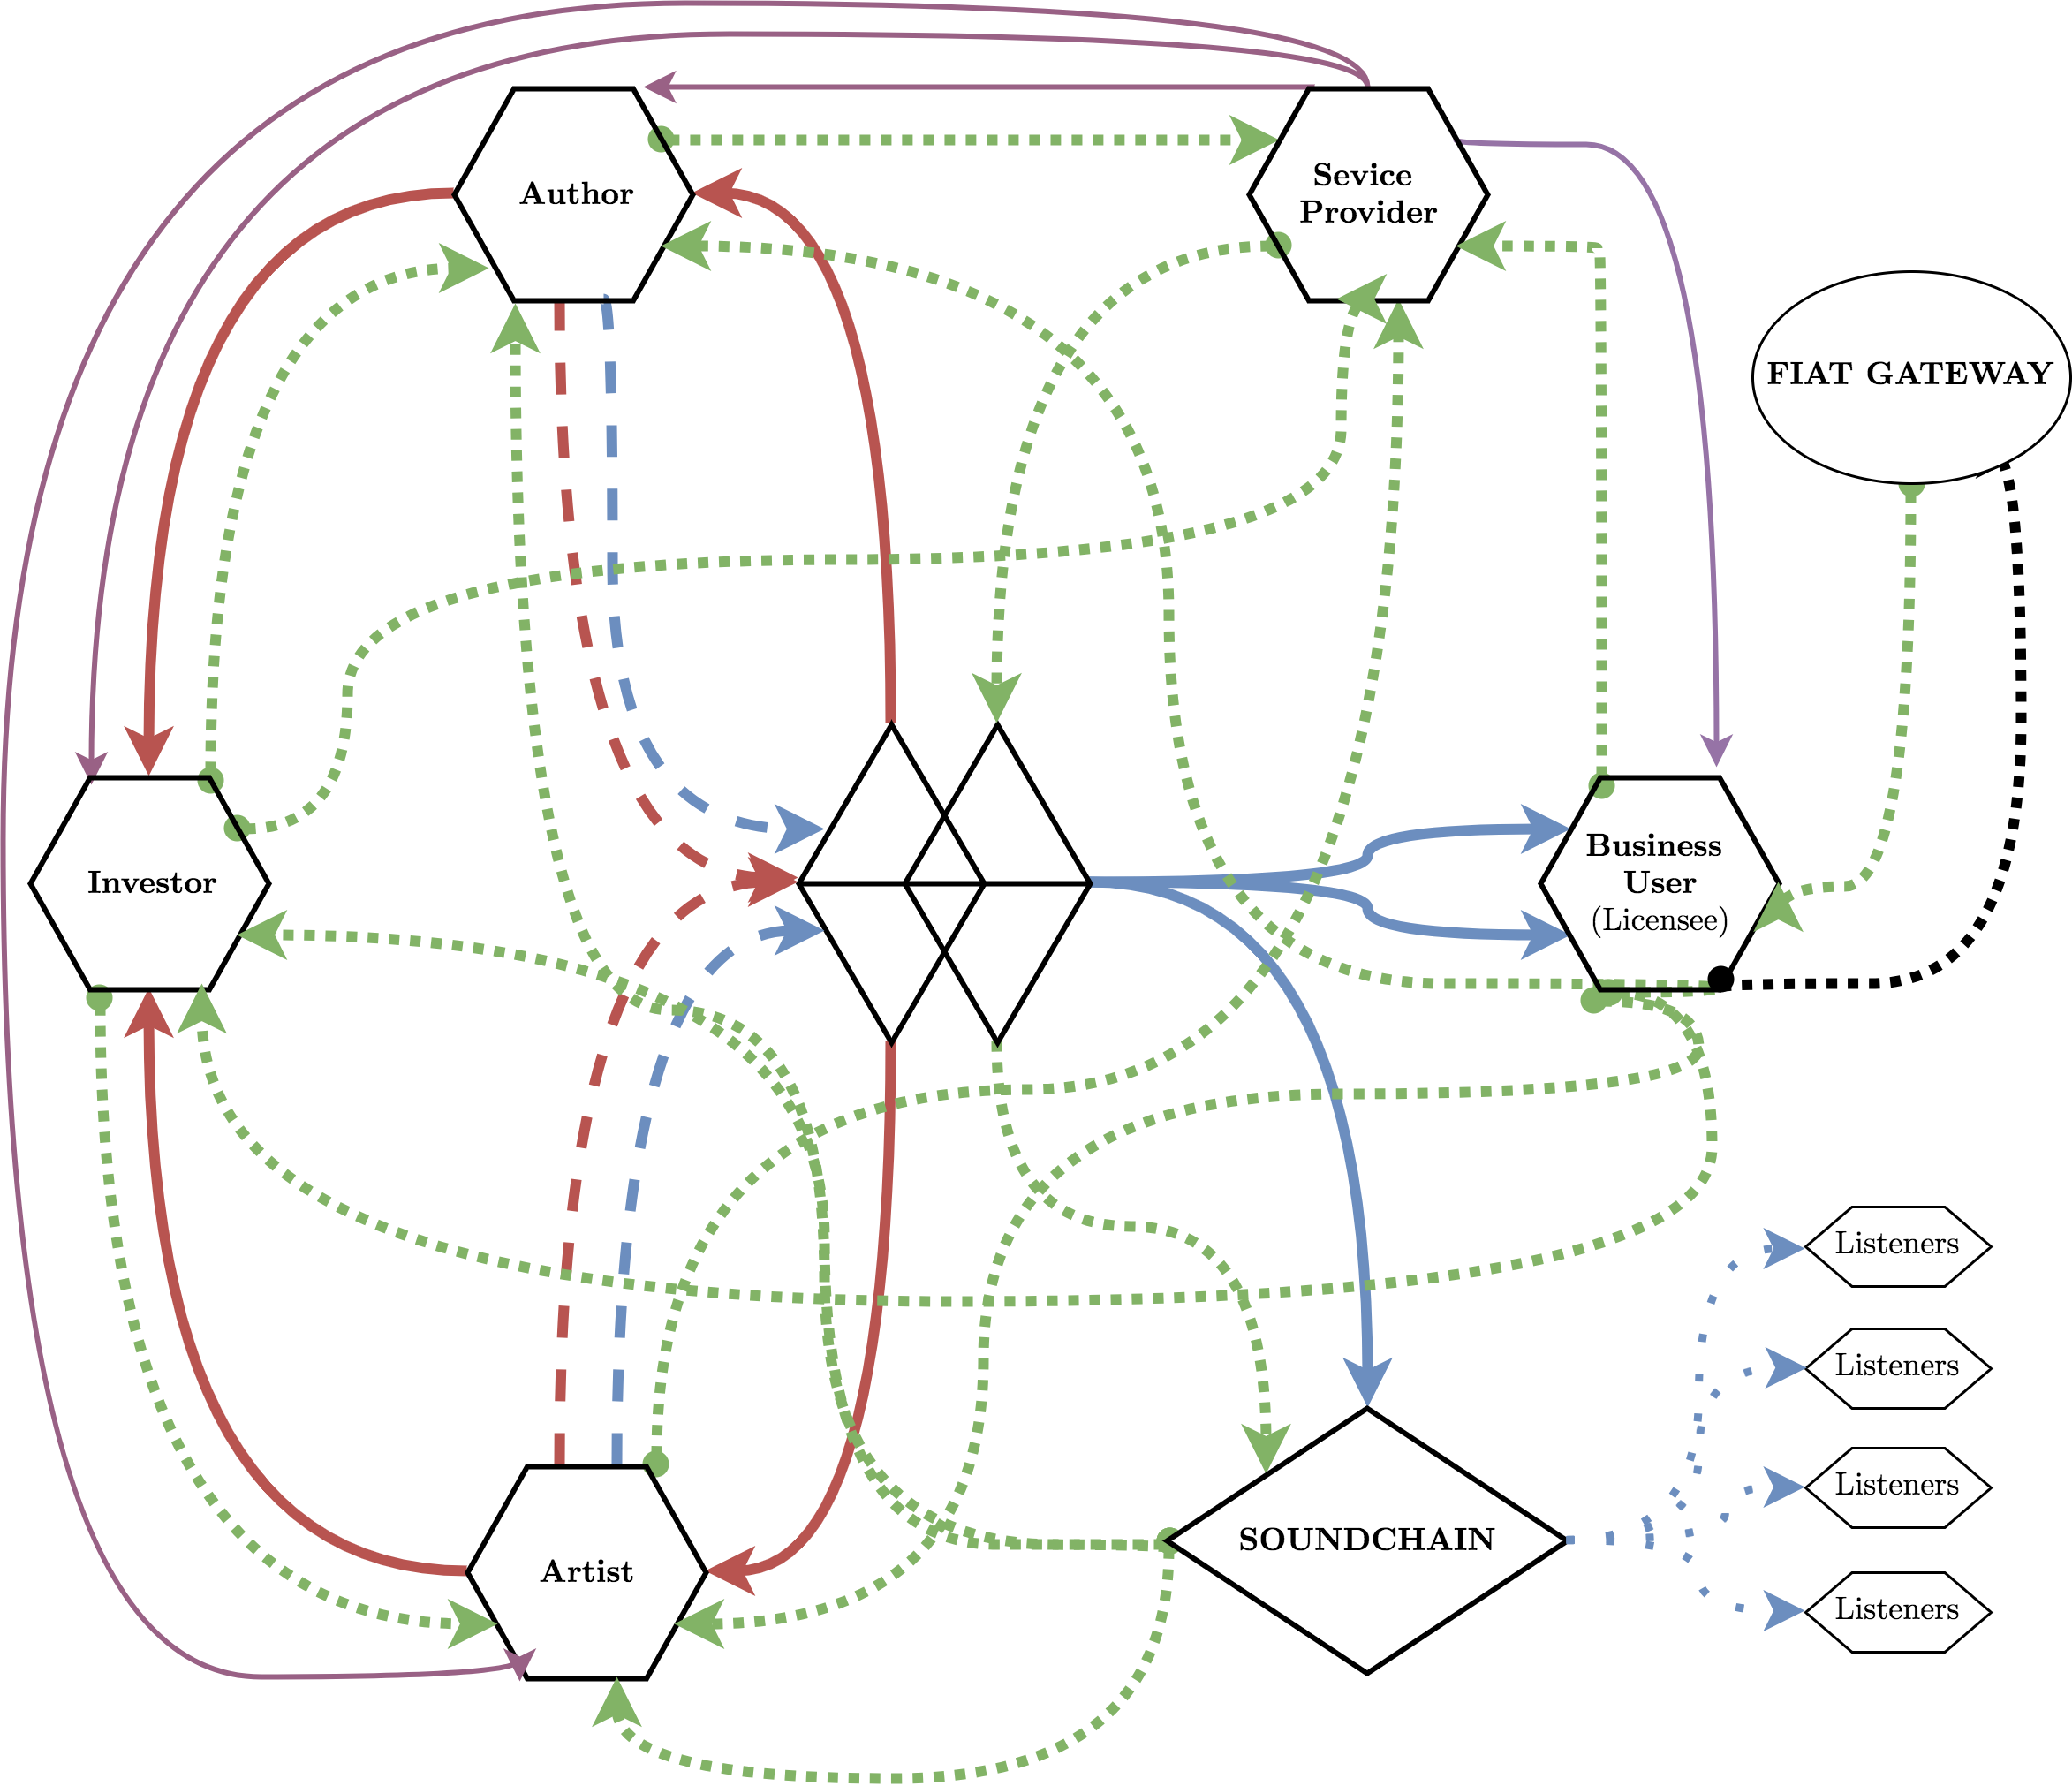
\includegraphics[width=\textwidth]{musereum-scheme}
\end{figure}
 
Every participant may have several roles at the platform – for example, a sound engineer may upload their own music as a creator, buy music tokens to support his fellow musicians, purchase collaboration licenses for their next projects, offer services at the service marketplace, listening to Madonna via the Soundchain player all along.

Furthermore, Musereum technology allows for the third-party developers to upload their own dApps within our system and create their own models of value creation for the industry.We try to create an infrastructure for different dapps to seamlessly run on top of Musereum blockchain, interacting with the Musereum IP database and utilizing ETM tokens to transfer value within the dapps and between them.

Musereum Platform is a system of digital products to solve core industry problem which described above.

Core platform products is:
\begin{itemize}
	\item \textbf{Decentralized Ledger}: Our decentralized ledger based on Ethereum source code, but with different consensus algorithm to avoid incurring transaction fees compare to Ethereum main-net.
	\item \textbf{Decentralized Virtual Machine} with cheap computation power. Move forward from PoW (see \hyperref[tech-blockchain]{Blockchain} to detail) allow to decrease cost of computation power and utilize decentralized network to solve more complex tasks such as \textit{searching}, \textit{indexing}, \textit{loop} over data.
	\item \textbf{Decentralized Content Network}: The current industry solutions  delivers their musical content from centralized content networks. In order to deliver on the promise as laid out in the business objectives, one deliverable is that of a decentralized system wherein many ecosystem participants could run nodes of the system and use consensus algorithms to synchronize
with one another.
	\item \textbf{Cryptocurrency}: The introduction of a cryptocurrency would enable a common exchange of value across all ecosystem participants globally. It would also serve to equalize the playing field and set a benchmark for services provided.
	\item \textbf{Transparent Rights Management} based on three core elements: musical assets, decentralized autonomous labels and licenses on smart-contracts.
	\item \textbf{Decentralized Exchange} without moment of authority to select what we trade and when. Any registered asset could to listing associated token as a tradable active.
	\item \textbf{Decentralized Marketplace} for the monetization of creativity through the sale of licenses.
	\item \textbf{Soundchain} One of the core dapps running on top of Musereum blockchain is the Soundchain. While the basic scenario of interacting with Musereum platform is the uploading of the music by the creator and tokenizing it, selling music tokens to investors and generating a royalty flow by licensing the music via the marketplace, the Soundchain will provide the participants with an alternative monetization model, at the same time letting them access the public with their music.
 
The Soundchain will comprise the streaming platform with the player interacting with the Pay-per-Play smart-contract. While the access to the uploaded music will be free to stream for every non-commercial user of the Soundchain player, the smart-contract will pay out a small royalty to the rights holders for every unique stream of their music. The PPP royalty rates will vary within the range of US \$0.01 to US \$2.00 equivalent in ETM, with the exact rate determined by several factors, the main one being the total price of licenses sold for the asset at the licensing marketplace.
 
The PPP royalties will be paid out of the Soundchain Foundation, to which 70\% of newly generated ETM tokens will be transferred - about 17.5 million ETM annually.
 
Soundchain would benefit the Musereum ecosystem in several ways. First of all, by subsidizing artists, we will attract more creators to the platform by providing them with a viable alternative to the existing streaming services. By allowing free streaming we will attract general public to the platform, and the statistics gathered this way will help rights holders to demonstrate the value of their music to potential business users of our platform. It will also serve as a promotion tool for musicians to acquire new audience, and will provide listeners with a convenient interface to directly acquire a commercial license or buy music tokens from the rights holders.

\end{itemize}
%\end{multicols}

\section{\hlc{Tools}}
\label{platform-tools}
%\begin{multicols}{2}
All of tools could be grouped by three categories:
\begin{enumerate}
	\item \textbf{Business and economy}. Core features provider here is \textit{Musereum Wallet}. Musereum Wallet is not just a wallet to hold and spend crypto-currency, it is default door to whole economy system of Musereum. 
	\item \textbf{Entertainment and listening}. Implements as a services around Musereum such as Soundchain to listen music for free.
	\item \textbf{Infrastructure}. Service and maintain level tools to monitoring, developing and auditing network. We are providing bunch of tools and services: blockchain explorer, deploy utilities, public http api and also.
\end{enumerate}
%\end{multicols}

\subsection{\hlc{Rights Management Tools}}
\label{platform-tools-rights}


\def\Registration{Person Registration (Author)}
\def\RegistrationMusereum{Create ETM Wallet}
\def\KYC{KYC (Proof of Identity)}
\def\CreateAsset{Create Asset}
\def\AssetTitle{Title}
\def\AssetImage{Image}
\def\AssetRelease{Release Date}
\def\AssetLanguage{Language}
\def\AssetBPM{BPM}
\def\AssetTempo{Tempo}
\def\AssetVocal{Vocal}
\def\AssetMusicalKey{Musical Key}
\def\AssetKeywords{Keywords}
\def\AssetMoods{Moods}
\def\AssetSimilar{Similar assets}
\def\AssetDescription{Description}
\def\AssetGenres{Genres}

\def\AssetRegistration{Create Asset Record}
\def\Registrator{Affilated Registrators}
\def\RegistrationBallot{Registration Ballot}
\def\AddAsset{Add Asset to Catalog}
\def\CreateDAL{Create Asset DAL}

\def\SetupDAL{Initial DAL Configuration}
\def\TokenSetup{DAL Token Setup}
\def\VotingSetup{DAL Voting Setup}

\begin{figure}[H]
\centering
\caption{DAL creation: Process 1}
\vspace{20pt}

\begin{tikzpicture}
\node(RegistrationMusereum) [rect, minimum width=6cm]
						{\RegistrationMusereum};
\node(KYC) 		[rect, minimum width=6cm, right=0.5cm of RegistrationMusereum.east]
						{\KYC};
\node(Registration) [above=0.5cm of RegistrationMusereum.north west, anchor=west]
						{\Registration};
						
\node(RegistrationRect) [rect, rounded corners, thick, fit={(RegistrationMusereum) (KYC) (Registration)}] {};

\node(AssetTitle) [rect, below=1.3cm of RegistrationMusereum.south west, anchor=north west]{\AssetTitle};
\node(AssetImage)[rect, below=0.2cm of AssetTitle.south]{\AssetImage};
\node(AssetRelease)[rect, below=0.2cm of AssetImage.south]{\AssetRelease}; 
\node(AssetLanguage)[rect, right=0.2cm of AssetTitle.east]{\AssetLanguage};
\node(AssetBPM)[rect, below=0.2cm of AssetLanguage.south]{\AssetBPM};
\node(AssetTempo)[rect, below=0.2cm of AssetBPM.south]{\AssetTempo};
\node(AssetVocal)[rect, right=0.2cm of AssetLanguage.east]{\AssetVocal};
\node(AssetMusicalKey)[rect, below=0.2cm of AssetVocal.south]{\AssetMusicalKey};
\node(AssetKeywords)[rect, below=0.2cm of AssetMusicalKey.south]{\AssetKeywords};
\node(AssetMoods)[rect, right=0.2cm of AssetVocal.east]{\AssetMoods};
\node(AssetSimilar)[rect, below=0.2cm of AssetMoods.south]{\AssetSimilar};
\node(AssetGenres)[rect, below=0.2cm of AssetSimilar.south]{\AssetGenres};

\path 
	let \p1=(AssetRelease.west), \p2=(AssetGenres.east)
	in node(AssetDescription) [
		rect,
		below=0.2cm of AssetRelease.south west,
		anchor=north west,
		minimum width=\x2-\x1-\pgflinewidth
	] {\AssetDescription};
	
\node(CreateAsset) [above=0.5cm of AssetTitle.north west, anchor=west]{\CreateAsset};
						
\node(CreateAssetRect) [rect, rounded corners, thick, fit={(CreateAsset) (AssetDescription)}] {};


\path 
	let \p1=(CreateAssetRect.south west), \p2=(CreateAssetRect.south east)
	in node(UploadProcess) [
		rect, thick, rounded corners,
		below=0.25cm of CreateAssetRect,
		minimum width=\x2-\x1-\pgflinewidth,
		text width=\x2-\x1-\pgflinewidth-40pt,
		inner sep=10pt
	] {\textbf{Encrypt and Upload to IPFS}};

\node(AssetRegistration) [rect, below=0.25cm of UploadProcess, xshift=-4cm]
						   {\AssetRegistration};
\node(RegistrationBallot) [check, aspect=3, below=0.25cm of AssetRegistration.south]
						   {\RegistrationBallot};
						   
\node(ForgetAsset) [rect, rounded corners, thick, right=1.5cm of RegistrationBallot, text width=5.5cm]
{\textbf{Unlink hash and release keepers}};
						   
\node(AddAsset) [rect, below=0.8cm of RegistrationBallot]
						   {\AddAsset};
						   
							   
\path 
	let \p1=(RegistrationMusereum.south west), \p2=(KYC.south east)
	in node(RegistryCertificate) [
		rect, thick, rounded corners,
		below=0.25cm of AddAsset,
		xshift=4cm,
		minimum width=\x2-\x1-\pgflinewidth,
		text width=\x2-\x1-\pgflinewidth-40pt,
		inner sep=10pt
	] {\textbf{Anchoring Right Registry Certificate to ETC Classic}};
						   
\path 
	let \p1=(RegistrationMusereum.south west), \p2=(KYC.south east)
	in node(CreateDAL) [
		rect, thick, rounded corners,
		below=0.25cm of RegistryCertificate,
		minimum width=\x2-\x1-\pgflinewidth,
		text width=\x2-\x1-\pgflinewidth-40pt,
		inner sep=10pt
	] {\textbf{Create and Setup Decentralized Autonomous Label}\linebreak\textit{Figure 3.2}};

\draw [thick, ->] (RegistrationMusereum) -- (KYC);
\draw [thick, ->] (RegistrationRect) -- (CreateAssetRect);
\draw [thick, ->] (CreateAssetRect) -- (UploadProcess);
\draw [thick, <-] (AssetRegistration.north) coordinate (p1) -- (UploadProcess.south -| p1);
\draw [thick, ->] (AssetRegistration) -- (RegistrationBallot);
\draw [thick, ->] (RegistrationBallot) --  node[fill=white] {fail} (ForgetAsset);
\draw [thick, ->] (RegistrationBallot) --  node[fill=white] {success} (AddAsset);
\draw [thick, ->] (AddAsset.south) coordinate (p1) -- (RegistryCertificate.north -| p1);
\draw [thick, ->] (RegistryCertificate) -- (CreateDAL);

\end{tikzpicture}
\end{figure}

\begin{figure}[H]
\centering
\caption{Create and setup Decentralized Autonomous Label}
\vspace{20pt}

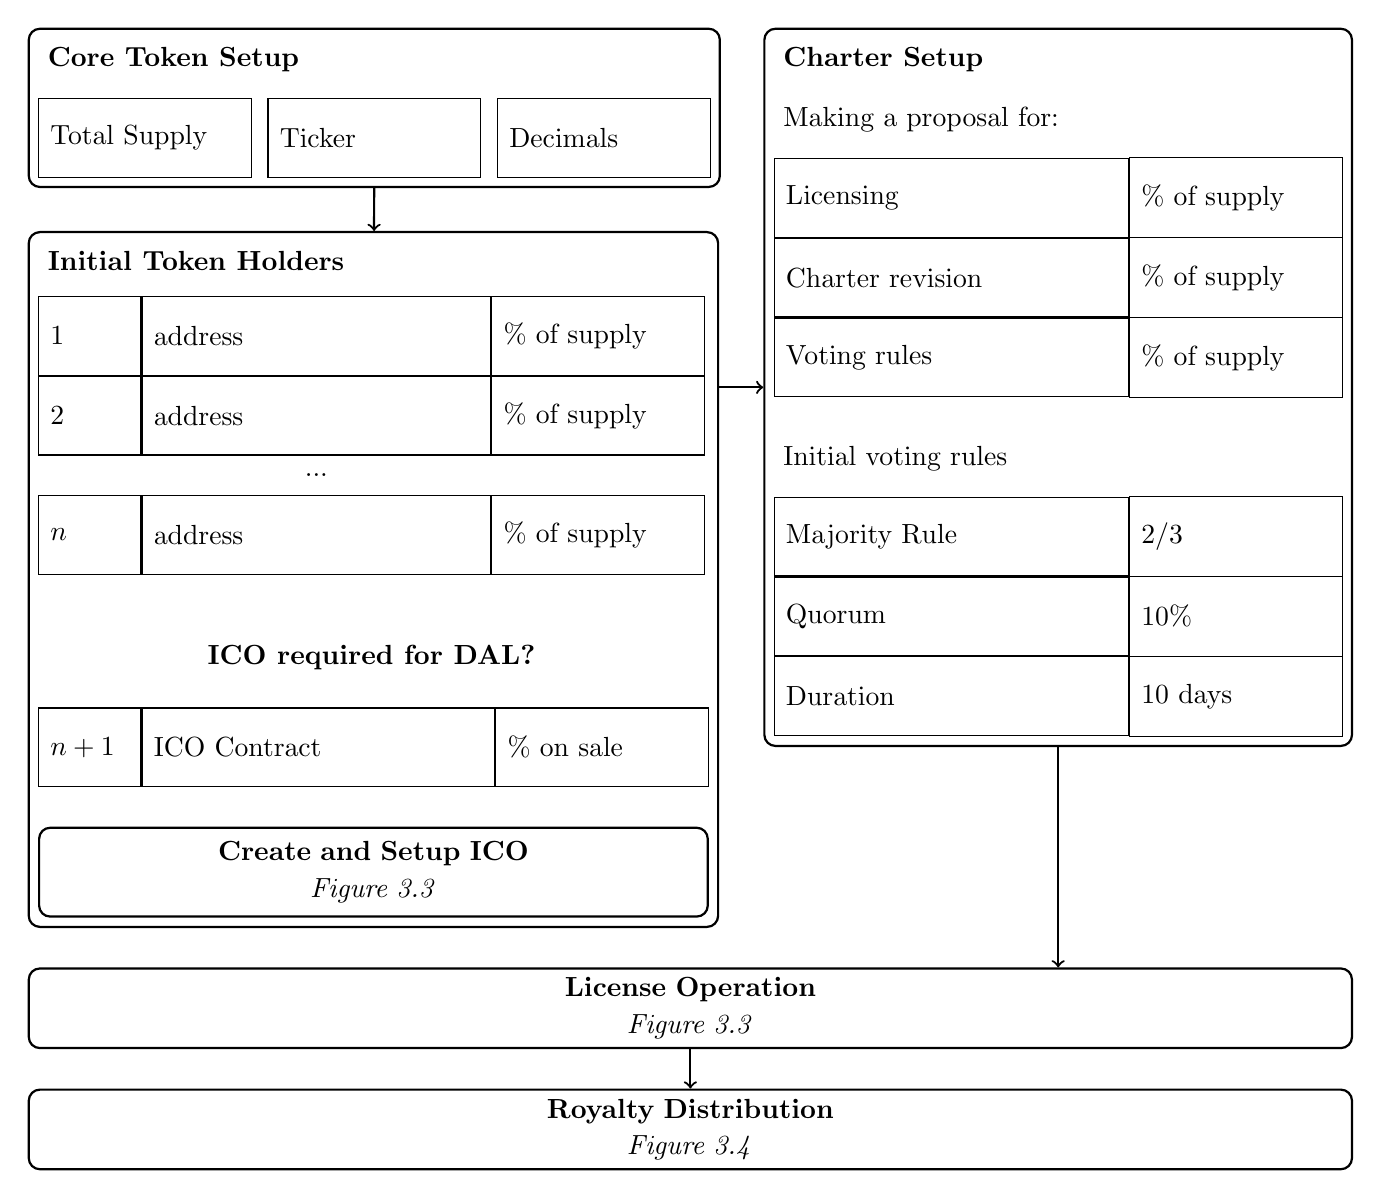
\begin{tikzpicture}	
\tikzset{%
	mini/.style = { rectangle, draw=black, minimum height=1cm, text width=2.4cm, inner sep=0.15cm },
	wrap/.style = {rectangle, draw=black, rounded corners, thick}
}
\node(ts1) [mini, yshift=15cm] {Total Supply};
\node(ts2) [above=0.2cm of ts1.north west, anchor=south west ] {\textbf{Core Token Setup}};
\node(ts3) [mini, right=0.2cm of ts1] {Ticker};
\node(ts4) [mini, right=0.2cm of ts3] {Decimals};
\node(tsr) [wrap, fit={(ts2) (ts4)}] {};

\node(ih0) [mini, below=1.5cm of ts1.south west, anchor=north west, text width=1cm] {1};
\node(ih3) [above=0.2cm of ih0.north west, anchor=south west ] {\textbf{Initial Token Holders}};
\path 
	let \p1=(ts1.south west), \p2=(ts4.south east)
	in node(ih1) [mini, right=0pt of ih0, text width=\x2-\x1-\pgflinewidth-4.4cm] {address};
\node(ih2) [mini, right=0pt of ih1] {\% of supply}; 

\node(ih0) [mini, below=0pt of ih0, text width=1cm] {2};
\path 
	let \p1=(ts1.south west), \p2=(ts4.south east)
	in node(ih1) [mini, right=0pt of ih0, text width=\x2-\x1-\pgflinewidth-4.4cm] {address};
\node(ih2) [mini, right=0pt of ih1] {\% of supply}; 

\node [below=0.1cm of ih1] {...};

\node(ih0) [mini, below=0.5cm of ih0, text width=1cm] {$n$};
\path 
	let \p1=(ts1.south west), \p2=(ts4.south east)
	in node(ih1) [mini, right=0pt of ih0, text width=\x2-\x1-\pgflinewidth-4.4cm] {address};
\node(ih2) [mini, right=0pt of ih1] {\% of supply}; 

\node(ih4) [fit={(ih3) (ih2)}] {};

%\node(ih5) [check, aspect=2, below=0.5cm of ih4] {ICO required for DAL?};
\node(ih5) [below=0.65cm of ih4] {\textbf{ICO required for DAL?}};
	
\path
	let \p1=(ih0.south west), \p2=(ih5.south west)
	in node(ih0) [mini, text width=1cm, anchor=north west, yshift=-0.35cm] at (\x1,\y2) {$n+1$};
\path 
	let \p1=(ts1.south west), \p2=(ts4.south east)
	in node(ih1) [mini, right=0pt of ih0, text width=\x2-\x1-\pgflinewidth-4.35cm] {ICO Contract};
\node(ih2) [mini, right=0pt of ih1] {\% on sale}; 

\path 
	let \p1=(ih0.south west), \p2=(ih2.south east)
	in node(ih6) [
		rect, thick, rounded corners,
		below=0.5cm of ih0.south west, 
		anchor=north west,
		minimum width=\x2-\x1-\pgflinewidth,
		text width=\x2-\x1-\pgflinewidth-10pt,
		inner sep=5pt
	] {\textbf{Create and Setup ICO}\linebreak\textit{Figure 3.3}};
	
\node(ihr) [wrap, fit={(ih3) (ih6)}] {};

\node(vs0) [right=0.8cm of ts4.north east, anchor=north west, text width=5cm] {Making a proposal for: };
\node(vsh) [above=0.2cm of vs0.north west, anchor=south west ] {\textbf{Charter Setup}};
\node(vs1) [mini, below=0.2cm of vs0.south west, anchor=north west, text width=4.2cm] {Licensing};
\path
	let \p1=(vs1.south), \p2=(vs1.north)
	in node(vs2) [
		mini,
		minimum height=\y2-\y1,
		right=0pt of vs1
	] {\% of supply};
	
\node(vs3) [mini, below=0pt of vs1, text width=4.2cm] {Charter revision};
\path
	let \p1=(vs3.south), \p2=(vs3.north)
	in node(vs4) [
		mini,
		minimum height=\y2-\y1,
		right=0pt of vs3
	] {\% of supply};
	
\node(vs5) [mini, below=0pt of vs3, text width=4.2cm] {Voting rules};
\path
	let \p1=(vs5.south), \p2=(vs5.north)
	in node(vs6) [
		mini,
		minimum height=\y2-\y1,
		right=0pt of vs5
	] {\% of supply};
	
	
\node(vs7) [below=0.5cm of vs5.south west, anchor=north west, text width=5cm] {Initial voting rules};
\node(vsA) [mini, below=0.2cm of vs7.south west, anchor=north west, text width=4.2cm] {Majority Rule};
\path
	let \p1=(vsA.south), \p2=(vsA.north)
	in node(vsB) [
		mini,
		minimum height=\y2-\y1,
		right=0pt of vsA
	] {$2/3$};
\node(vsA) [mini, below=0pt of vsA, text width=4.2cm] {Quorum};
\path
	let \p1=(vsA.south), \p2=(vsA.north)
	in node(vsB) [
		mini,
		minimum height=\y2-\y1,
		right=0pt of vsA
	] {10\%};
\node(vsA) [mini, below=0pt of vsA, text width=4.2cm] {Duration};
\path
	let \p1=(vsA.south), \p2=(vsA.north)
	in node(vsB) [
		mini,
		minimum height=\y2-\y1,
		right=0pt of vsA
	] {10 days};
	
\node(vsr) [wrap, fit={(vsh) (vsB)}] {};

\path
	let \p1=(ihr.west), \p2=(vsr.east)
	in node(dop) [
		wrap,
		text centered,
		below=0.5cm of ihr.south west,
		anchor=north west,
		text width=10cm,
		minimum height=1cm,
		minimum width=\x2-\x1-\pgflinewidth
	] {\textbf{License Operation}\linebreak\textit{Figure 3.3}};
	
\path
	let \p1=(ihr.west), \p2=(vsr.east)
	in node(royalty) [
		wrap,
		text centered,
		below=0.5cm of dop,
		text width=10cm,
		minimum height=1cm,
		minimum width=\x2-\x1-\pgflinewidth
	] {\textbf{Royalty Distribution}\linebreak\textit{Figure 3.4}};
	
\draw [thick, ->] (tsr) -- (ihr);
\draw [thick, <-] (vsr.west) coordinate (p1) -- (ihr.east |- p1);
\draw [thick, ->] (vsr.south) coordinate (p1) -- (dop.north -| p1);
\draw [thick, ->] (dop) -- (royalty);
\end{tikzpicture}
\end{figure}

\begin{figure}[H]
\centering
\caption{License creation process}
\vspace{20pt}
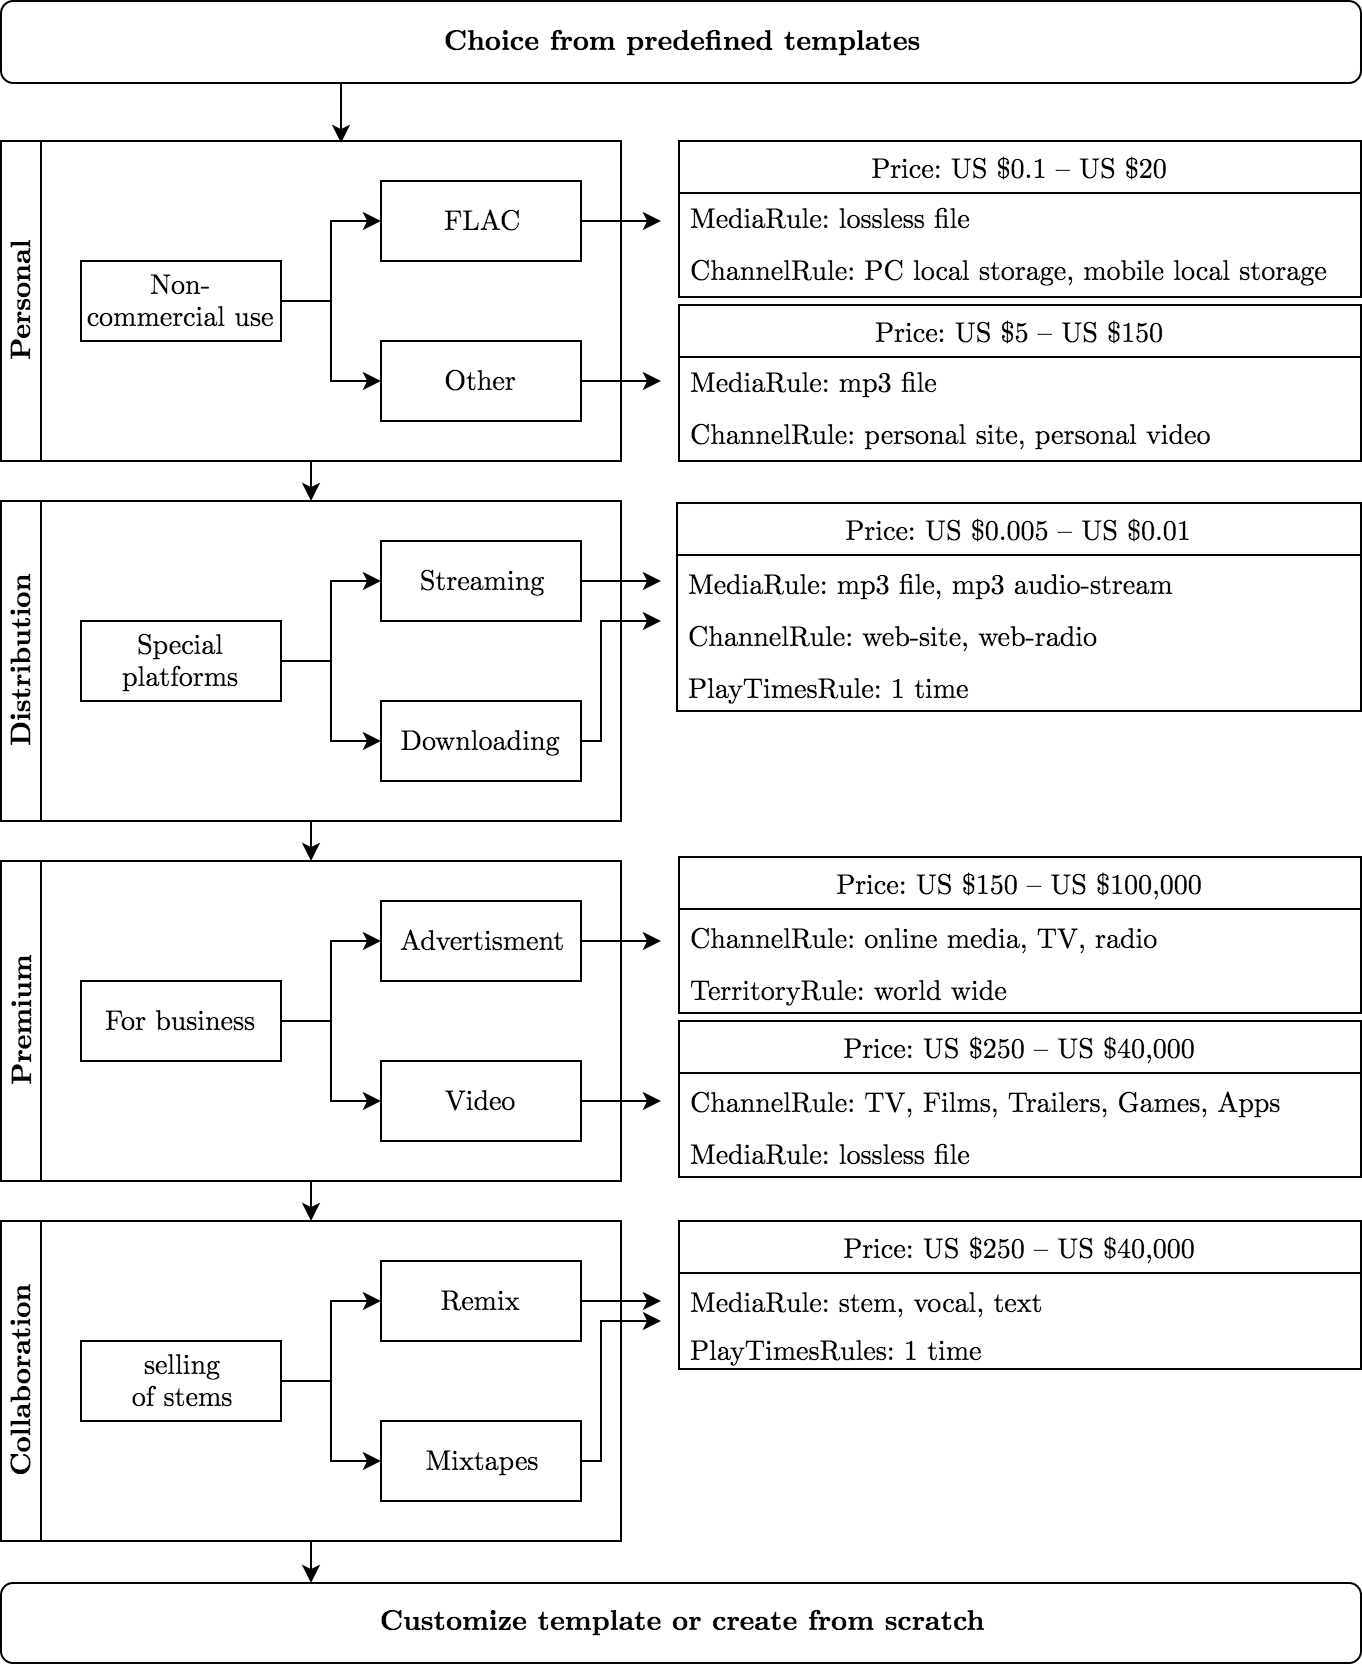
\includegraphics[width=\textwidth]{licensing}
\end{figure}

\begin{figure}[H]
\centering
\caption{Royalty Distribution}
\vspace{20pt}
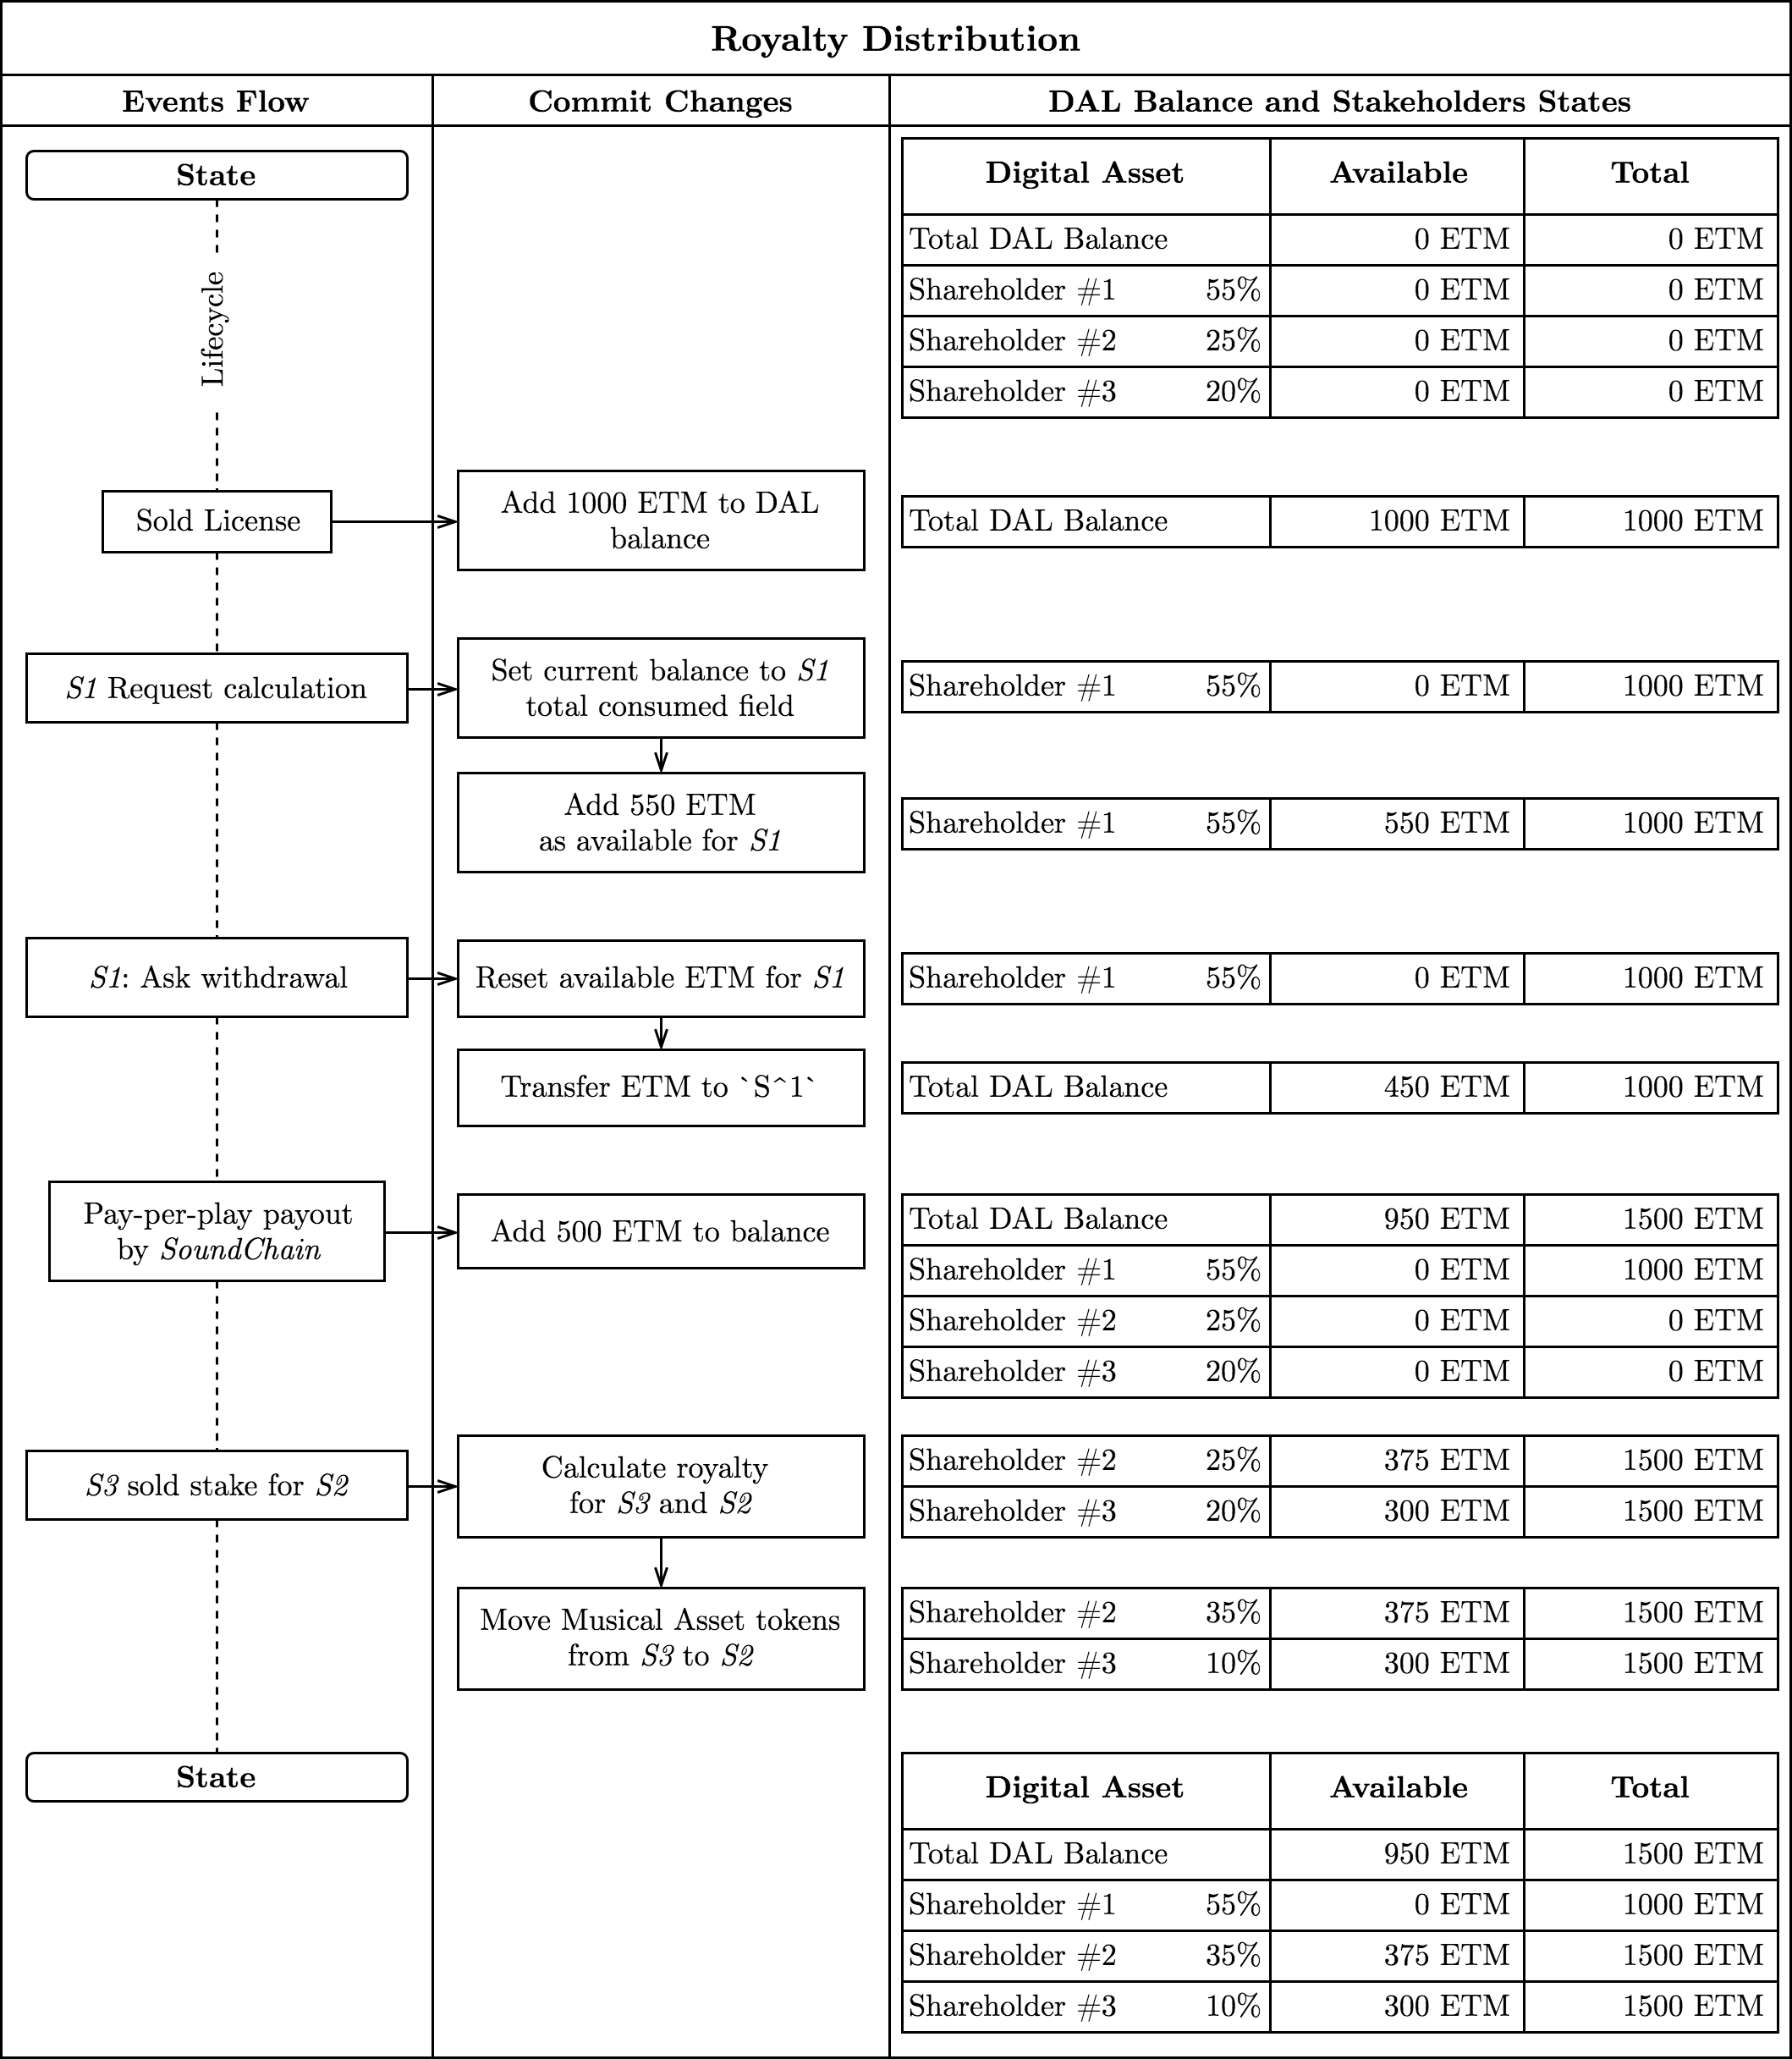
\includegraphics[width=\textwidth]{royalty}
\end{figure}

\section{Roles}
\label{platform-roles}
In a nature of platform users could identify yourself with desired roles as well as delegate roles to others.

Primary platform select next core roles:
\begin{itemize}
	\item \textbf{User} is the person who create an account on the platform and got permissions to hold and transfer ETM and interact with a musical catalog.
	\item \textbf{Person} is the user who provide proof-of-personality to receive permissions to invest and trade with a musical assets.
	\item \textbf{Artist} is a person with at least one registered musical asset on a platform. Should be at least person to register asset.
	\item \textbf{Notary} is the person chosen for the production of blocks
	\item \textbf{Affilated specialist} is the person chosen to do some important work for the platform. 
	\item \textbf{Keeper} is the user provided storage to store musical content.
\end{itemize}

\chapter{Technical Description of Platform}
\section{Overview}
\label{tech-review}
%\begin{multicols}{2}
Musereum protocol tasks can be divided into the folllowing components:
\begin{itemize}
\item Providing unified system state without central computing for reliable operation;
\item Decentralized big data storage that is censor-proof due to inability to block a unified (centralized) data source;
\item Providing proof of system integrity for change history auditing;
\item Interface for making changes in the future state of the system.
\end{itemize}
%\vfill\null\columnbreak
Application of the "Blockchain concept" using Ethereum Virtual Machine (EVM) provides monitoring and changing single state of Musereum system without the need to use centralized computing (see \hyperref[tech-blockchain]{Blockchain} for detail). IPFS technology is applied to store big data volumes (audio tracks, metadata, text and graphical description) \textit{(see \hyperref[tech-storage]{Decentralized Storage} for more detail)}.

%\end{multicols}
%\pagebreak
\subsection{Naming convention}
\label{tech-review-naming}
%\begin{multicols}{2}
Here and elsewhere all entities with defined content or interface will get a short mathematical name with a common rule: \textit{capital latin letter except for N, B, Z}, e. g:

\begin{equation}
Y \ \text{is Notary}
\end{equation}

All globally defined contracts will be assigned to a lowercase Greek symbol, e. g. Notary Registry Contract – $\nu$ and a special record associated with certain function of the contract:

\begin{equation}
\nu \ \text{is Notary Registry Contract}
\end{equation}
\begin{equation}
\nu_{vote} \ \text{is vote contract method}
\end{equation}
%\vfill\null
%\columnbreak

Sets of all known entities are defined as accepted entity name in a blackboard record except for $\mathbb{N}, \mathbb{B}, \mathbb{Z}$, e. g.: list of notaries:

\begin{equation}
\mathbb{Y} \ \text{is set of all known Notaries}
\end{equation}

$\mathbb{N}$ – set of all integers within the range $(0; 2^{256} - 1)$. $\mathbb{N}_1$ – subset $\mathbb{N}$ without 0.

$\mathbb{Z}$ – set of all integers within the range $(-2^{255}; +2^{255} - 1)$.

$\mathbb{B}$ – is a set of all bytes $(0; 255)$. 

$\mathbb{X}^{i}$ – is a set of dimension $i$ where every set member belongs to $\mathbb{X}$, e.g.:
\begin{equation}
\mathbb{B}^{32} \text{ is a set of } \mathbb{B} \text{ with size } 32
\end{equation}

Obtaining the set member can be described in two ways: with a subindex or in square brackets:
\begin{equation}
\begin{aligned}
\mathbb{Y}_2 = \mathbb{Y}[2] \\
\mathbb{Y}_n = \mathbb{Y}[n] 
\end{aligned}
\end{equation}

External data is represented in the formulae as members of set $\Gamma$with readable names (or abbreviations if mentioned), e. g.: Global time in UNIX format:
\begin{equation}
\Gamma_{time} \ \text{is world time variable}
\end{equation}

All \hlc{temporal} variables in formulae are written as latin letters, e. g.:
\begin{equation}
\begin{aligned}
\text{Let } a \text{ is a second notary in list of notaries} \\
a = \mathbb{Y}[2]
\end{aligned}
\end{equation}
%\end{multicols}

\subsection{Mathematical functions and symbols}
\label{tech-review-math}
%\begin{multicols}{2}
All formulae apply $|\mathbb{Y}|$ as an operator of number of $\mathbb{Y}$-set elements.

The following conventions and functions are applied to reduce and/or make a mathematical notation readable:

\textbf{Search index in set} – $\mathcal{I}$:
\begin{align}
&\ \text{Let } a \text{ is a set of values: } \nonumber\\
a =&\ {100, 200, 300} \nonumber\\
f(v, x) =&\ \{i \ | \ i \in \mathbb{N},  i > |v|, v_i = x \} \\
\mathcal{I}(v, x) =&\ \begin{cases}
	min(f(v,x)), & \text{if } |f(v, x)| > 0 \\
	-1, & \text{overwise}
\end{cases}
\\
\\
r1 = &\ \mathcal{I}(a, 200) = 1\nonumber \\
r2 = &\ \mathcal{I}(a, 400) = -1
\end{align}

\textbf{\hlc{Determining} named tuple} – $\mathcal{O}$:
\begin{align}
&\ \text{Let } a \text{ is a set of names: } \nonumber\\
a =&\ \{name, age, height\} \nonumber\\
&\ \text{and let } b \text{ is a set of indexes: } \nonumber\\
b =&\ \{0, 1, 2\} = \{x \ | \ x \in \mathbb{N}, x < |a|\} \\
& \nonumber\\
&\ \text{finaly } r \text{ is a target named tuple, where} \nonumber\\
r =&\ \mathcal{O}(a) = \mathcal{O}(name, age, height) \\ 
r =&\ \{x_i \ | \ i \in  a, x_i = 0 \}
\end{align}

\textbf{\hlc{Determining} event tuple } – $\mathcal{E}$:\hfill\null\linebreak
Special defined tuple containing target data and general data for every event: \code{event}, \code{txHash}, \code{txIndex}, \code{blockHash}, \code{blockHeight}, \code{address}.
\begin{align}
&\ \text{Let } a \text{ is a set of default event fields: } \nonumber\\
a =&\ \{event, txHash, txIndex, blockHash, blockHeight, address\} \nonumber\\
&\ \text{Let } b \text{ is a set of extra event fields: } \nonumber\\
b =&\ \{asset, index\} \nonumber\\
&\ \nonumber\\
&\ \text{finaly } e \text{ is a target event tuple, where} \nonumber\\
r =&\ \mathcal{E}(b) \\
r =&\ \mathcal{O}(\{asset, index\} \ \cup \ a)
\end{align}
%\end{multicols}

%\pagebreak
\section{Platform architecture}
\label{tech-arch}
%\begin{multicols}{2}
The primary aim of the platform is to provide users with capabilities to:
\begin{enumerate}
\item Read and interpret data
\item \hlc{Commit} changes
\item Search data
\item Audit and receive proof of data \hlc{integrity}
\end{enumerate}
The platform is divided into the following logic layers in order to provide above-mentioned capabilities:
\begin{itemize}
	\item \hyperref[tech-arch-underlayer]{Storage and \hlc{ledger}}
	\begin{itemize}
		\item \hyperref[tech-blockchain]{Blockchain}
		\item \hyperref[tech-storage]{Decentralized storage}
	\end{itemize}
	\item \hyperref[tech-arch-connect]{Read and write \hlc{layer}}
	\begin{itemize}
		\item \hyperref[tech-arch-connect-nodes]{Public nodes}
		\item \hyperref[tech-arch-connect-validators]{Notary nodes}
	\end{itemize}
	\item \hyperref[tech-arch-interfaces]{Interaction interfaces}
	\begin{itemize}
		\item \hyperref[tech-arch-interfaces-dapp]{Decentralized application}
		\item \hyperref[tech-arch-interfaces-api]{Application Programming Interface}
	\end{itemize}
\end{itemize}
%\end{multicols}

\def\Interface{Interaction Interface}
\def\Connect{Access layer}
\def\Underlayer{Storage and ledger layer}

\def\DApps{Decentralized Applications}
\def\Api{API}
\def\Requests{Direct \hlc{requests}}

\def\RPC{Musereum RPC}
\def\Nodes{Public nodes}
\def\Notaries{Notaries}
\def\EVM{Ethereum Virtual Machine}
\def\Blockchain{Blockchain ledger}
\def\IPFS{IPFS}
\def\ReadWrite{Read and write}
\def\ReadOnly{Read only}

\begin{center}
\begin{tikzpicture}[node distance=1.5cm]
\node (DApps) 					[rect]
										{\DApps};
\node (Api)						[rect, right=0.2cm of DApps]
										{\Api};
\node (Requests)				[rect, right=0.2cm of Api]
										{\Requests};
\node (Interface)				[above=0.5cm of DApps.north west, anchor=west] {\Interface};										

\node (InterfaceRect)		[rect, rounded corners, dashed, fit={(Interface) (DApps) (Api) (Requests)}] {};

\path 
	let \p1=(DApps.west), \p2=(Requests.east)
	in node(RPC) [
		rect,
		below=1.5cm of DApps.south west,
		anchor=north west,
		minimum width=\x2-\x1-\pgflinewidth
	] {\RPC};
    
\path 
	let \p1=(RPC.west), \p2=(RPC.east)
	in node(Nodes) [
		rect,
		below=0.4cm of RPC.south west,
		anchor=north west,
		minimum width=(\x2-\x1-\pgflinewidth)
	] {\Nodes};
    
\path 
	let \p1=(Nodes.west), \p2=(Nodes.east)
	in node(Notaries) [
		rect,
		below=1.8cm of Nodes.south west,
		anchor=north west,
		minimum width=(\x2-\x1-\pgflinewidth)/2-0.3cm
	] {\Notaries};
    
\draw 
	let \p1=(Nodes.south), \p2=(Notaries.north) 
	in [arrow] (\x2,\y1) -- node [fill=white] {\ReadWrite} (Notaries.north);
	
\draw [arrow] (RPC) -- (Nodes);

\node (Connect)			[above=0.5cm of RPC.north west, anchor=west] {\Connect};
\node (ConnectRect)		[rect, rounded corners, dashed, fit={(RPC) (Nodes) (Notaries) (Connect)}] {};

\draw [thick] (Nodes) -- node [fill=white, yshift=15pt]{\ReadOnly} (ConnectRect.south);

\path
	let \p1=(Nodes.west), \p2=(Nodes.east)
	in node(EVM) [
		rect, 
		below=1.5cm of Notaries.south west,
		anchor=north west,
		minimum width=(\x2-\x1-\pgflinewidth)/2-0.1cm
	] {\EVM};
	
\path
	let \p1=(Nodes.west), \p2=(Nodes.east)
	in node(Blockchain) [
		rect, 
		below=0.4cm of EVM.south west,
		anchor=north west,
		minimum width=(\x2-\x1-\pgflinewidth)/2-0.1cm
	] {\Blockchain};
\path
	let \p1=(Nodes.west), \p2=(Nodes.east),
	     \p3=(EVM.north), \p4=(Blockchain.south)
	in node(IPFS) [
		rect, 
		below=0pt of EVM.north east,
		anchor=north west,
		xshift=0.2cm,
		minimum width=(\x2-\x1-\pgflinewidth)/2-0.1cm,
		minimum height=(-\y4+\y3)
	] {\IPFS};
\node (Underlayer)			[above=0.5cm of EVM.north west, anchor=west] {\Underlayer};
\node (UnderlayerRect)		[rect, rounded corners, dashed, fit={(EVM) (Blockchain) (IPFS) (Underlayer)}] {};
    
\draw [arrow] (EVM) -- (Blockchain);
\draw [arrow] (InterfaceRect) -- (ConnectRect);
\draw [arrow] (ConnectRect) -- (UnderlayerRect);
\end{tikzpicture} 
\end{center}

\subsection{Storage and record layer}
\label{tech-arch-underlayer}
%\begin{multicols}{2}
Storage and record layer is the basic layer of the platform. The layer provides capability to keep a decentralized state ledger (blockchain) and to store big amounts of data.

Every layer element: blockchain, storage and virtual machine are distributed among the network (nodes) and everyone can create a personal local copy.
%\end{multicols}
\subsection{Access layer}
\label{tech-arch-connect}
%\begin{multicols}{2}
Access layer application: providing data from the basic layer on request and receiving change requests.

Creating a node for an additional access point is not limited and available for anyone. This feature is a benefit that distinguishes Musereum platform from other centralized music platforms:

\begin{itemize}
	\item It provides 100\% network up-time
	\item It is Censor-proof
	\item Stakeholders can create a personal local copy of the network without necessity to trust third parties
\end{itemize}
%\end{multicols}
%\pagebreak
\subsection{Interaction interface layer}
\label{tech-arch-interfaces}
%\begin{multicols}{2}
Interaction interface layer is the top layer of the platform. The layer receives user input and generates requests applicable with protocol. Requests are divided into two types: read and write.

Reading data from the blockchain and the decentralized storage is not limited. The only requirement is to form a request according to API agreement.

In order to write (changing state, saving data), a user must provide valid request signature based on his or her unique private key as well as follow other writing requirements (rights, funds for protocol operation etc.).

It is not required for an organization to have its own access point (synchronize a node with the network) in order to make a request; a serverless web-application can be used as a client \textit{(see \hyperref[tech-apps]{Decentralized applications} for detail)}.

%\end{multicols}
\section{Blockchain}
\label{tech-blockchain}
%\begin{multicols}{2}
Musereum protocol is an open public blockchain that requires permission to generate blocks and is based on Ethereum protocol.


\subsection{Ethereum}
\label{tech-blockchain-evm}
Ethereum is an open-source, public, blockchain-based distributed computing platform featuring smart contract (scripting) functionality. It provides a decentralized Turing-complete virtual machine, the Ethereum Virtual Machine (EVM), which can execute scripts. "Gas", an internal transaction pricing mechanism, is used to mitigate spam and allocate resources on the network.
\subsection{Ethereum Smart-contracts}
\label{tech-blockchain-contracts}
Smart contracts are deterministic exchange mechanisms controlled by digital means that can carry out the direct transaction of value between untrusted agents. They can be used to facilitate, verify, and enforce the negotiation or performance of economically-laden procedural instructions and potentially circumvent censorship, collusion, and counter-party risk. In Ethereum, smart contracts are treated as autonomous scripts or stateful decentralized applications that are stored in the Ethereum blockchain for later execution by the EVM. Instructions embedded in Ethereum contracts are paid for in ether (or more technically "gas") and can be implemented in a variety of Turing complete scripting languages.
\subsection{Musereum rules for EVM interaction}
\label{tech-blockchain-rules}
%\begin{multicols}{2}
In order to improve security of platform participants, interaction with EVM smart contracts in Musereum differs from that in parental Ethereum network.

Any member of the network can upload a smart contract to the network, but such smart contract has $P_{development}$ status and it is available for interaction with affiliated addresses of network accounts. Initially this address belongs to the account of the user who uploaded the contract.

Smart contract interaction rules are regulated by allowance smart contract: $\rho$.

Any smart contract call initially requests allowance to make the call – $\rho_{allowTx}(T_{from}, T_{to})$
%\end{multicols}
\begin{align}
a &= \rho_{stateOf}(T_{to}) \nonumber\\
b &= \rho_{affilateWith}(T_{to}) \nonumber\\
\rho_{allowTx}(T_{from}, T_{to}) &= \begin{cases}1, & \text{if } a = P_{production} \\ 1, & \text{if } a = P_{development} \wedge T_{from} \in b \\ 0, & \text{overwise} \end{cases}
\end{align}
The author of a smart contract must provide source code for a check and pass the checking procedure in order to get $P_{production}$ status \textit{(see for details \hyperref[tech-apps-contracts-registry]{Smart Contract Registry})}

% Nodes
\def\Owner{Владелец контракта}
\def\Blockchain{Блокчейн}
\def\Registry{Реестр контрактов}
\def\LoadByteCode{Uploading byte code to blockchain}
\def\LoadSourceCode{Uploading source code}
\def\ValidationEnded{Code \hlc{Validation is} passed?}
\def\ChangeStatus{Changing smart contract state}

\begin{center}
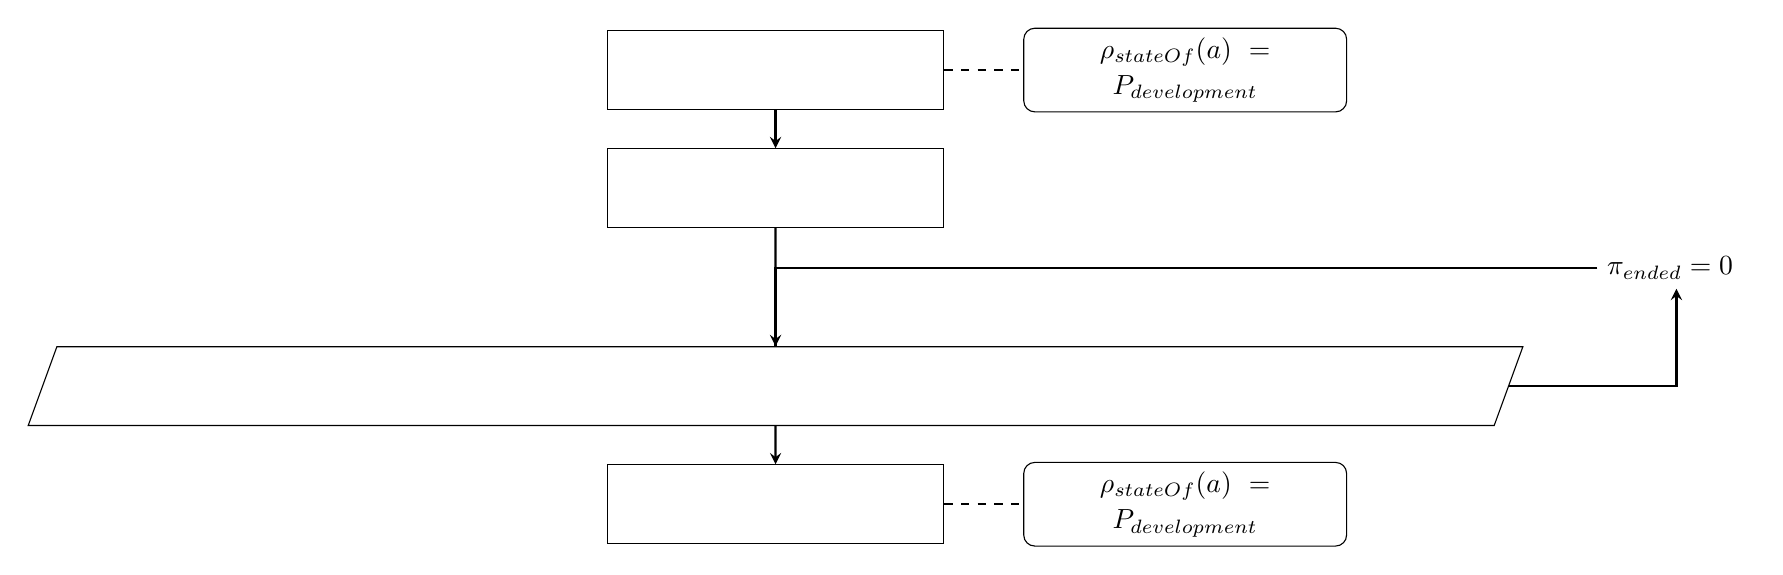
\begin{tikzpicture}[node distance=1.5cm]
\node (LoadByteCode)		[rect, text width=11.5em] 
										{\LoadByteCode};

\node (LoadSourceCode)	[rect, text width=11.5em, below of=LoadByteCode] 
										{\LoadSourceCode};

\node (ValidationEnded)	[event, text width=11.5em, below=1.5cm of LoadSourceCode]
										{\ValidationEnded};
										
\node (aux0)[right=2cm of ValidationEnded]{};
\node (Invalid)					[text width=5em, above of=aux0]
										{$\pi_{ended} = 0$};

\node (ChangeStatus)		[rect, text width=11.5em, below of=ValidationEnded]	
										{\ChangeStatus};

\node (InDevelopment)		[inout, text width=11em, right=1cm of LoadByteCode]			
										{$\rho_{stateOf}(a) = P_{development}$};
										
\node (InProduction)			[inout, text width=11em, right=1cm of ChangeStatus]			
										{$\rho_{stateOf}(a) = P_{development}$};

%arrows
\draw [arrow] (LoadByteCode)				-- (LoadSourceCode);
\draw [-, thick, dashed]
	(LoadByteCode)								--(InDevelopment);
\draw [arrow] (LoadSourceCode) 			-- (ValidationEnded);
\draw [arrow] (ValidationEnded)			-- (ChangeStatus);
\draw [arrow] (ValidationEnded)			-| (Invalid);
\draw [thick]  (Invalid)  							-| (ValidationEnded);
\draw [-, thick, dashed] 
	(ChangeStatus)									-- (InProduction);

\end{tikzpicture} 
\end{center}

\subsection{Proof-of-Authority}
\label{tech-blockchain-inexpensive}

Consensus for a single network state in a decentralized block generator structure is achieved by Proof-of-Authority (hereafter PoA) algorithm. Achieving consensus through PoA requires:
\begin{enumerate}
\item A common list of notaries ($\mathbb{Y}$) permitted to generate blocks;
\item Notary Registry Contract ($\nu$).
\end{enumerate}
The list of notaries can be changed (excluding / appointing notaries) by Notary Registry Contract based on results of active notary voting (majority).

\textit{Initially, 12 notaries are listed.}

Notary \hlc{duties}: 
\begin{enumerate}
\item Validate transactions received from system participants,
\item \hlc{Write changed state to a new block},
\item \hlc{Sign block chain} with a personal crypto-signature.
\end{enumerate}

In order to maintain consensus, an external constant $\Gamma_{step}$ is introduced, it defines the number of seconds in one time step or time between blocks. Musereum defines constant $\Gamma_{step}$ as 5 or 1 block every five seconds.
\begin{equation}
\Gamma_{step} = 5
\end{equation}
According to PoA consensus algorithm, a notary has the right to generate one block ($K$) in $a$ \hlc{timestamps} $\Gamma_{time}$. If $a$ is a number of notaries:
\begin{equation}
a = |\mathbb{Y}|
\end{equation}
Notary index $i$ is selected from set $\mathbb{Y}$ to create a block on time stamp $b$according to the formula: 
\begin{equation}
b = \frac{\Gamma_{time}}{\Gamma_{step}},  \quad b \in \mathbb{N} 
\end{equation}
\begin{equation}
i = b \ mod \ a
\end{equation}
%\end{multicols}
\subsection{Version selection}
\label{tech-blockchain-score}
%\begin{multicols}{2}
In case if notaries fail to achieve global (single) system state and a fork or creating two or more blockchains takes place ($\mathbb{K}$), the network defines the score ($\beta_{score}(\mathbb{K}_c)$) of every  chain based on the number of notaries participating in \hlc{chain creation}:	
%\vfill\null\columnbreak
\begin{align}
h &= |\mathbb{K}_c| & \quad h \ \text{is length of blockchain} \\
\beta_{score}(\mathbb{K}_c) &= \Gamma_{u128max} * h - m
\end{align}
The network always selects the chain with the highest score according to $\beta_{score}$.
%\end{multicols}
\subsection{Block finalization}
\label{tech-blockchain-fin}
% \begin{multicols}{2}
According to consensus, the block in the chain after which more than 50\% of notaries have generated 2 or more blocks is considered irreversable.

Thus, the minimal time for complete block validation ($C$) is:
\begin{equation}
C = 2 * \Gamma_{step} * |\mathbb{Y}|
\end{equation}
\textit{Or 120 seconds with default protocol settings: 12 notaries with 1 block every five seconds}
% \end{multicols}
\subsection{Notary Witness}
\label{tech-blockchain-confirmation}
%\begin{multicols}{2}
In order to do any activity that requires changing system state, user must form a transaction ($T$) signed with a unique cryptographic signature ($T_{sign}$). 

The crypto-signature is a warrant for the network that proves owner's will to create a transaction using creator's account. 

The notary in turn to generate a block checks the validity of a transaction and executes the related code:
\begin{enumerate}
\item Sender has the right to create a transaction for the given address – $\rho_{allowTx}(T_{from}, T_{to})$ \textit{(see \hyperref[tech-blockchain-rules]{EVM Interaction Rules} for detail)}
\item Transaction meets formal criteria – $\rho_{initialValid}(T)$
\item Checking account owner's signature – $\rho_{checkSign}(T)$
\item Checking sufficient amount of tokens on ETM account to pay in advance for computer operation – $\rho_{upFront}(T)$
\item Execution of related	EVM code	did not 	throw an exception $\rho_{exception}(\rho_{execute}(T))$
\end{enumerate}
%\end{multicols}
\begin{align}
\rho_{success}(T) = 	&\rho_{allowTx}(T_{from}, T_{to}) &> 0 \ \wedge \\
 								&\rho_{initialValid}(T) &> 0 \ \wedge \\
								&\rho_{checkSign}(T) &> 0 \ \wedge \\
								&\rho_{upFront}(T) &> 0 \ \wedge \\
 								&\rho_{exception}(\rho_{execute}(T)) &= 0
\end{align}
%\begin{multicols}{2}
Having validated the transaction, notary packs the transaction in blocks and informs the network about the block and change of the network state ($\mathbb{W}_h$).
\begin{equation}
\mathbb{W}_h = \rho_{state}(\mathbb{W}_{h-1}, \mathbb{K}_h)
\end{equation}
Other notaries receive the block, check it ($\rho_{success}(T)$) and take decision to accept it to the chain. By creating a block on $\mathbb{K}_h$ the notary validates the block and all included transactions.
Thus, the transaction may have from 1 to $|\mathbb{Y}|$ validating signatures.
Minimal time for receiving $|\mathbb{Y}|$ signatures:
\begin{equation}
a = \Gamma_{step} * |\mathbb{Y}|
\end{equation}
%\end{multicols}
%\vfill\null\pagebreak

\subsection{Crosschain communication and Ethereum Classic}
\label{tech-blockchain-anchoring}
%\begin{multicols}{2}
To increase the security and fault tolerance of the network, Musereum periodically duplicates key information about the network and core-events in an external blockchain that is not controlled by notaries.

As an anchoring blockchain for storing key information, the Ethereum Classic network was chosen, for the following reasons:
\begin{itemize}
	\item Total market cap – US~\$1,811,306,656.00
	\item The cost of 51\% attack on the network is more than US~\$40,000,000
	\item Permission-less consensus – Proof-of-Work.
\end{itemize}

Musereum duplicates to the Ethereum Classic:
\begin{enumerate}
	\item Hashes of each $n$-block to provide proof of historical data;
	\item The facts of key transactions: the registration of musical assets, the purchase of licenses.
\end{enumerate}
%\end{multicols}

\begin{figure}[H]
\centering
\caption{Crosschain communication}
\vspace{20pt}
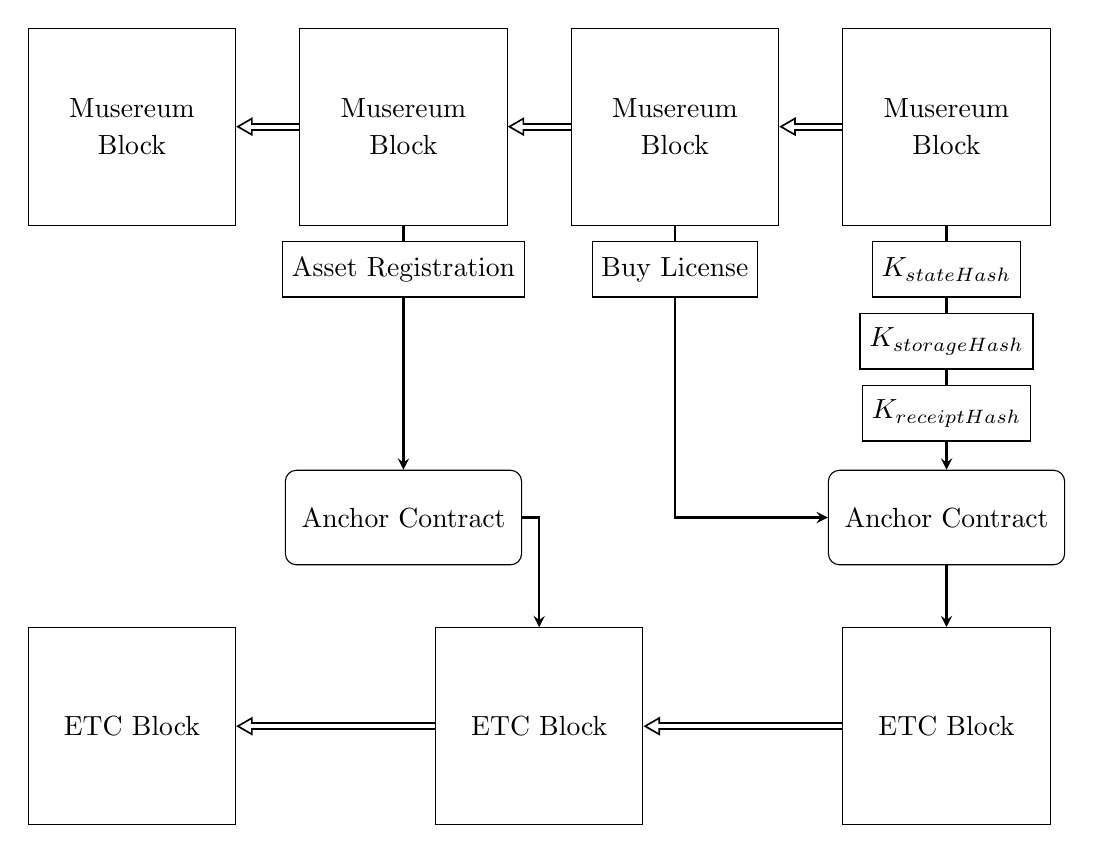
\begin{tikzpicture}
\tikzset{%
	part/.style = { rectangle, draw=black, minimum height=.7cm },
	block/.style = { rectangle, draw=black, minimum height=2.5cm, minimum width=2.5cm, text width=2.4cm, text centered},
	event/.style = { rectangle, , rounded corners, draw=black, text centered},
	anchoring/.style = { rectangle, rounded corners, draw=black, text centered, minimum width=3cm, minimum height=1.2cm}
}
\node(BlockA)			[block]
								{Musereum \linebreak Block};
\node(BlockB)			[block, right=0.8cm of BlockA.east]
								{Musereum \linebreak Block};
\node(BlockC)			[block, right=0.8cm of BlockB.east]
								{Musereum \linebreak Block};
\node(BlockD)			[block, right=0.8cm of BlockC.east]
								{Musereum \linebreak Block};
								
\node(NewAsset)		[part, below=0.2cm of BlockB.south]
								{Asset Registration};
\node(BuyLicense)	[part, below=0.2cm of BlockC.south]
								{Buy License};
\node(StateHash)		[part, below=0.2cm of BlockD.south]
								{$K_{stateHash}$};
\node(StorageHash)	[part, below=0.2cm of StateHash.south]
								{$K_{storageHash}$};
\node(ReceiptHash)	[part, below=0.2cm of StorageHash.south]
								{$K_{receiptHash}$};
						
								
\node(ETCA)				[block, below=5.1cm of BlockA.south]
								{ETC Block};
\node(ETCC)				[block, below=5.1cm of BlockD.south]
								{ETC Block};			
\node(ETCB) 			[block] at ($(ETCA)!0.5!(ETCC)$) 
								{ETC Block};

\node(AnchoringA)	[anchoring,  below=3.1cm of BlockB.south]
								{Anchor Contract};
								
\node(AnchoringB)	[anchoring,  below=3.1cm of BlockD.south]
								{Anchor Contract};


%\draw[->] (manufacturer.south) -- ++(-.5,0) -- ++(0,-1) -|  (retailer1.north);	
%\draw[myarrow] (manufacturer.south) -- ++(.5,0) -- ++(0,-1) -|  (retailer2.north);

\draw [line]		(BlockB) -- (NewAsset);
\draw [arrow]	(NewAsset) 	-- (AnchoringA);
\draw [arrow] 	(AnchoringA) -| (ETCB);

\draw [line]		(BlockD) --	
						(StateHash) --
						(StorageHash) -- 
						(ReceiptHash);
						
\draw [line	]		(BlockC) -- (BuyLicense);
						
\draw [arrow] 	(ReceiptHash) 	-- 	(AnchoringB);
\draw [arrow] 	(BuyLicense)		|- 	(AnchoringB);
\draw [arrow] 	(AnchoringB)		-- 	(ETCC);


\draw [vecArrow] 	(BlockD) -- (BlockC);
\draw [vecArrow] 	(BlockC) -- (BlockB);
\draw [vecArrow] 	(BlockB) -- (BlockA);
\draw [innerWhite](BlockD) -- (BlockC);
\draw [innerWhite](BlockC) -- (BlockB);
\draw [innerWhite](BlockB) -- (BlockA);

\draw [vecArrow] 	(ETCC) -- (ETCB);
\draw [vecArrow]	(ETCB) -- (ETCA);
\draw [innerWhite](ETCC) -- (ETCB);
\draw [innerWhite](ETCB) -- (ETCA);
							
\end{tikzpicture}
\end{figure}

\subsection{Block Generation Reward}
\label{tech-blockchain-reward}
%\begin{multicols}{2}
Block reward ($R$) consists of two parts: new emission and activity fees.

Musereum platform implies emission of new ETM tokens by creation of a block. Emission is limited to 3 ETM per block.

Amount of activity fee is calculated independently for each transaction. The sender indicates in transaction difficulty unit price ($T_{gasPrice}$) that he or she is ready to spend to compensate network operation.

Final 	fee is calculated according to formula:
\begin{equation}
x = T_{gasPrice} * \rho_{dificulty}(\rho_{execute}(T))
\end{equation}

Total block reward:
\begin{align}
&\text{Let } a \text{ is a list of transactions of block } \mathbb{K}_h \\
a &= \mathbb{K}[h]_{transactions} \\
\mathbb{R}_h &= 3 + \sum\limits_{i=0}^{|a|} a_i
\end{align}
%\end{multicols}

\subsubsection{Reward distribution}
\label{tech-blockchain-reward-distribution}
Apart from Ethereum and Bitcoin protocols, Musereum network has no miners – the primary value is created by artists who select Musereum platform for publication and distribution of music.

Musereum highly appreciates artitsts' contribution to platform integrity and it sends the most part of block reward to fund artists.

General distribution pattern:

\def\Musereum{Musereum}
\def\Development{Platform Development}
\def\Infrastructure{Infrastructure}

\begin{figure}[H]
\centering
\caption{Block reward distribution}
\vspace{20pt}
\begin{tikzpicture}[scale=3]

\newcounter{c}
\newcounter{d}
\foreach \p/\t in {
	80/\Musereum,
	10/\Development, 
	10/\Infrastructure}
  {
    \setcounter{c}{\value{d}}
    \addtocounter{d}{\p}
    \slice{\thec/100*360}
          {\thed/100*360}
          {\p\%}{\t}
  }

\end{tikzpicture}
\end{figure}

\begin{itemize}
	\item 80\% – Musereum:
	\begin{itemize}
		\item 90\% – SoundChain Foundation \textit{(see more in \hyperref[tech-apps-soundchain-payperplay]{Pay-per-Play})}
		\item 10\% – bounty programs: Fans Bounty, Clipmaker Bounty and etc.
	\end{itemize}
	\item 10\% – Platform Development Foundation
	\item 10\% – \hlc{Network Infrastructure}
	\begin{itemize}
		\item 25\% – Notaries / Validators
		\item 25\% – \hlc{Keepers}
		\item 25\% – Affilated specialists (\hlc{registrators} and smart-contract auditors)
		\item 25\% – Oracles
	\end{itemize}
\end{itemize}

\section{Decentralized Storage}
\label{tech-storage}
\subsection{Overview}
\label{tech-storage-review}
\textit{InterPlanetary File System} (IPFS) is a peer-to-peer network connecting remote servers in a single global decentralized storage platform. A significant amount of storage capacity will be required to store all the compositions in a decentralized manner and this can be achieved through IPFS.

Musereum is planning to utilize customized Clustered IPFS Swarm for the platform. Clustered IPFS nodes should create the necessary storage capacity for storing beats, compositions and videos, while providing faster access to them. Files stored in IPFS are divided into smaller chunks and each chunk is encrypted with keys. Based on our experience, storing files as chunks can significantly reduce download time and make them more secure.

The Musereum community will be involved in storing and streaming of the compositions and gain rewards in return from emission rate of ETM tokens.
\subsection{Naming System}
\label{tech-storage-naming}
Musereum is planning to utilize \textit{The Inter-Planetary Naming System} (IPNS) to provide simple way to stored files. 

It allows you to store a reference to an IPFS file under the namespace of corresponding KeeperID (the hash of keeper's public key).

\section{Decentralized Applications}
\label{tech-apps}
Musereum DApps implement the code for record and storage layer as well as the interaction interface code. The protocol allows DApps to interact.

\subsection{Governance dApp}
\label{tech-apps-governance}
%\begin{multicols}{2}
Musereum starts from initial ceremony to set up a list of Notaries.

During the initial ceremony a master of ceremony creates a set of keys for each validator. He/She distributes them to validators one by one. Before each distribution of keys, he/she sends a transaction to a smart contract with a list of validators. That smart contract is used by consensus algorithm to determine if a validator has rights to participate in consensus and create blocks. The validator’s smart contracts are used by other DApps, e.g. Governance DApp and Payout DApp.

A validator generates three keys in the Initial Ceremony DApp:
\begin{itemize}
	\item mining key, required to participate in consensus and create blocks.
	\item voting key, required to create ballots and vote on ballots.
	\item payout key, not required. Used in Payout DApp to send daily mined coins from the mining key to the payout key. If a mining node should be compromised, an attacker will get daily earnings or less.
\end{itemize}

All keys are generated on the client side and not transmitted over the Internet without a validator’s permission and willingness. When keys are generated, the validator stores them on secure local storage, e.g. saves them to a hardware wallet and the password to a password manager. The validator signs a transaction to the validator’s contract with the initial key, provided by the master of ceremony.

Initial ceremony is a required procedure to start a new network based on Oracles Network’s ideas of independent validators.
%\end{multicols}

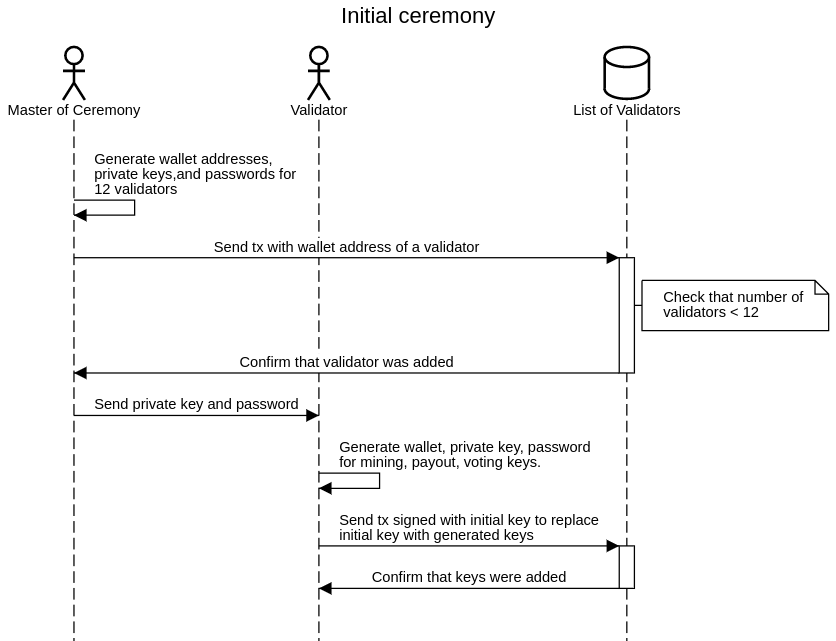
\includegraphics[width=\textwidth]{initial}

%\begin{multicols}{2}
Futurе changes of Notaries List will be committed through voting. Creation of voting ballot based on a request with assign form.

Valid notary of the Oracles Network fills out a form in DApp providing:
\begin{itemize}
	\item mining key - mining key of a new or existing notary, which will be voted on
affected key type - key type (mining, payout, or voting key) of a new or existing notary, which will be voted on
	\item memo - brief information about notary, which will be voted on
	\item action - add affected key to the network or remove it from the network
\end{itemize}

If the affected key type is mining key, the user will be asked to provide personal data of the notary (owner of this mining key) such as full name, physical address, U.S. state name, zip code, notary license ID, and notary license expiration date.

At the final step, one transaction to create a new ballot in Oracles contract will be pushed to the blockchain to add a new ballot after the user presses “Continue” button. It should be noted, that in case of a mining key, it will be two consistent transactions: to add personal data of a notary and a new ballot to contract. User will see MetaMask popups equal to the number of transactions. After the confirmation and successful mining of the transaction by existing validators, the user will see the created ballot in the list and be able to vote on it. 
%\end{multicols}

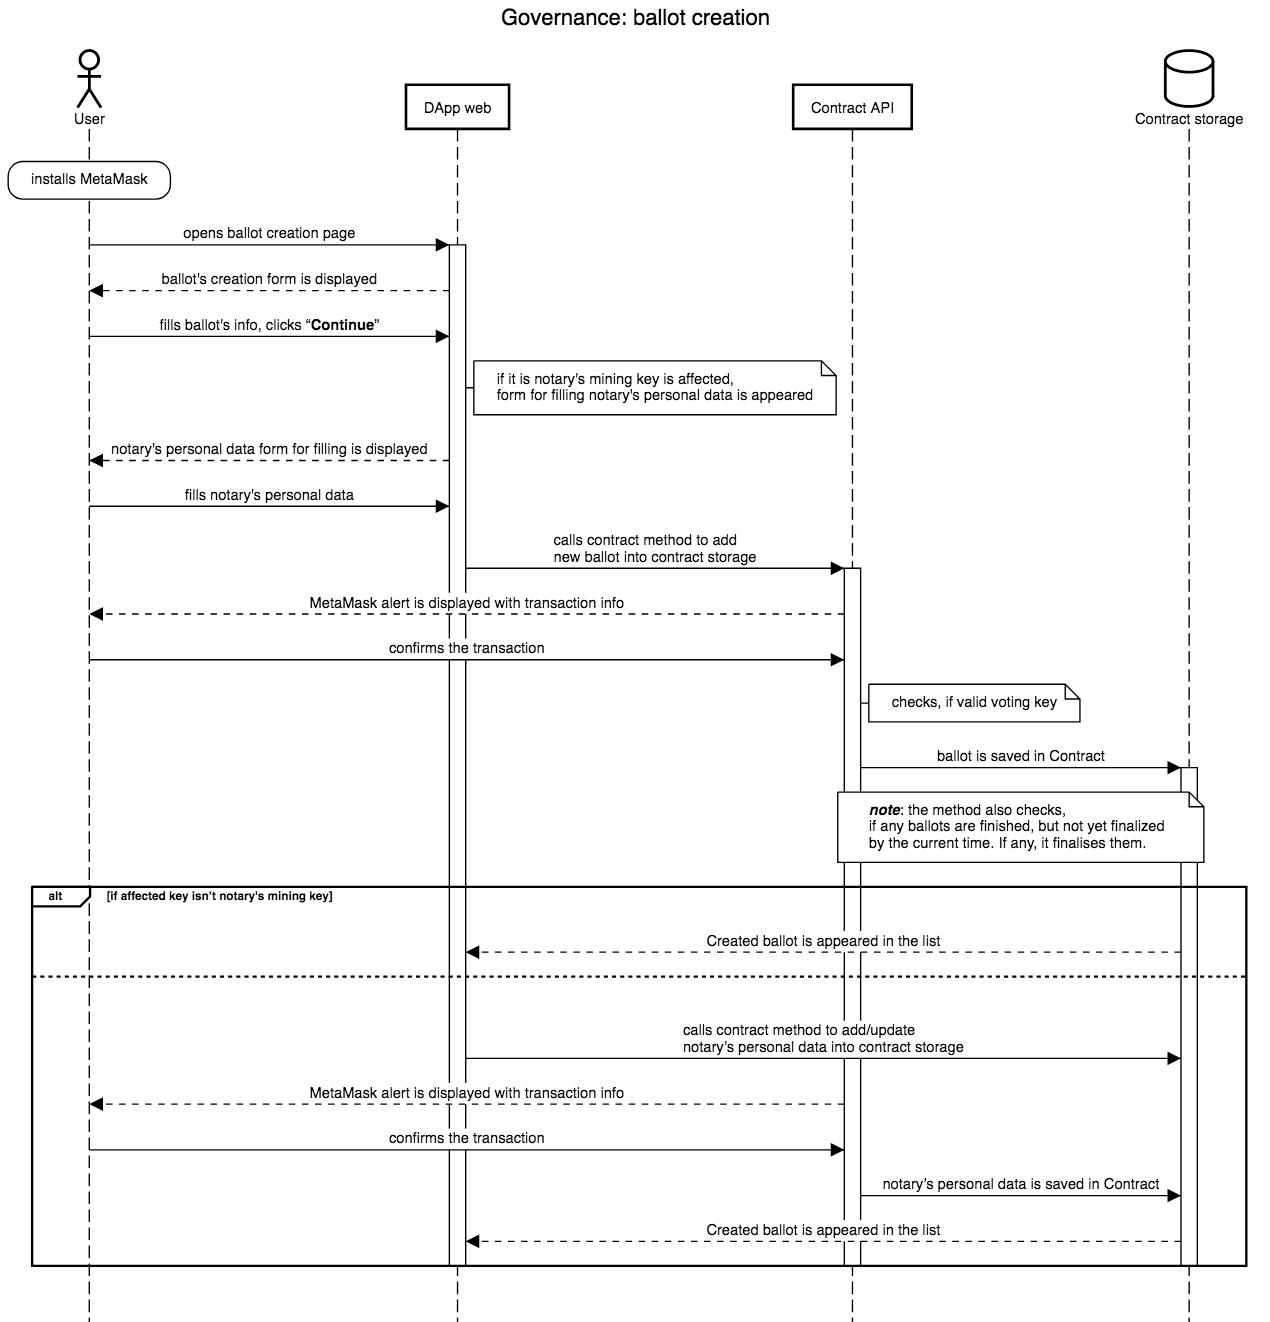
\includegraphics[width=\textwidth]{creation-ballot}

\subsection{Contract Registry}
\label{tech-apps-contracts-registry}
%\begin{multicols}{2}
The DApp for registering and recording smart contracts of the platform.

The DApp smart contract allows to receive:
\begin{enumerate}
	\item The list of all registered smart contracts
	\item Smart contract state associated with the address:
	\begin{enumerate}
		\item \code{Unknown} – unknown state (default for unknown addresses in \hlc{Contract Registry })
		\item \code{Development} – smart contract is registered but currently is under development (interaction is allowed for affiliated users only)
		\item \code{Production} – smart contract is registered and \hlc{ready to interact}
		\item \code{Halt} – smart contract is registered but halted (by author's decision)
		\item \code{Suspend} – smart contract is registered but suspended (by auditor's decision)
	\end{enumerate}
\item A link to a source code repository
\item A link to ABI JSON for smart contract interaction
\item The list of affiliated auditors
\item A ballot \hlc{instance} to take decision about changing the state \textit{(see \hyperref[tech-apps-voting]{VotingDApp} for detail)}
\end{enumerate}
%\end{multicols}
\subsubsection{Source code and smart contract checking}
\label{tech-apps-contracts-validate}
%\begin{multicols}{2}
Smart contracts are validated in three ways:
\begin{itemize}
	\item Source code validation for:
		\begin{enumerate}
			\item Vulnerabilities 
			\item Compliance with stated business logic
			\item Absence of algorithmic errors
		\end{enumerate}
	\item Compliance with law applicable to Musereum platform
	\item Compliance with Musereum concept
\end{itemize}
%\vfill\null\columnbreak
In order to approve a smart contract, all affiliated auditors must have a unanimous consent for all three points.

Validation process can be monitored in \hyperref[tech-apps-voting]{Voting dApp} in corresponding\code{ContractValidationBallot}.
%\end{multicols}
\subsection{Musereum Name System (MNS)}
\label{tech-apps-mns}
%\begin{multicols}{2}
The Ledger of names associated with addresses in Musereum platform is required to provide access to up-to-date protocol apps avoiding the necessity to remember the internal address (20-character hex-address).

Name record can be created by any network user for a random address. Number of names for the address is unlimited.

In order to protect names from improper use, the registration of a new name is charged in ETM according to the current price.

Name record is a MNS-derived smart contract: \code{NameRecordContract}.

The smart contract contains the data about the name owner and associated network address and provides the following capabilities:
\begin{itemize}
	\item for the owner to change the associated address;
	\item for the owner to change the owner (transfer of right)
\end{itemize} 

MNS limits available names: 
\begin{itemize}
	\item Name length cannot exceed 20 characters (or less if non-ASCII characters are used) 
	\item Name length cannot be shorter than 4 characters
\end{itemize}
%\end{multicols}
\subsubsection{Interaction interface}
\label{tech-apps-mns-api}
\code{mapping (address => address) names} – ($\eta_{names}$)\hfill\null\linebreak
List of addresses associated with addresses of name registration smart contracts

\code{uint price} – ($\eta_{price}$)\hfill\null\linebreak
Name registration price in ETM tokens

\code{event NewName(address indexed name, byte20 ascii)} – ($\eta_{NewName}$)\hfill\null\linebreak
\hlc{Event log} of new name registration

\code{event AssociateWith(address indexed name, address indexed target)} – ($\eta_{AssociateWith}$)\hfill\null\linebreak
Event log of address associating with name registration smart contract

\code{function buyName(byte20 acsii) payable} – ($\eta_{buy}$)\hfill\null\linebreak
Method to buy name. Returns \code{address} if the buying is successful and \code{throw} in case of error.

\begin{equation}
\eta_{buy}(s) = \begin{cases}
	throw, & \text{if } s \in \eta_{NewName} \\ 
	throw, & \text{if } |s| < 4 \\
	throw, & \text{if } T_{value} < \eta_{price} \\
	address, & \text{overwise}
\end{cases}
\end{equation}

\paragraph{Smart-contract NameRecord}– ($\eta'$)

\code{address owner} – ($\eta'_{owner}$)\hfill\null\linebreak
Current name owner

\code{byte20 ascii} – ($\eta'_{ascii}$)\hfill\null\linebreak
Registered name (typicaly is 20 ASCII letter)

\code{address target} – ($\eta'_{target}$)\hfill\null\linebreak
Current association with address on Musereum platform

\code{function associate(address target)} – ($\eta'_{associate}$)\hfill\null\linebreak
Change name association to the new address. Returns \code{true} if successful and \code{throw} in case of error.
 
\begin{equation}
\eta'_{associate}(a) = \begin{cases}
	throw, & \text{if } T_{from} \neq \eta'_{owner} \\
	throw, & \text{if } a = 0 \\
	true, & \text{overwise}
\end{cases}
\end{equation}

\subsection{Voting dApp}
\label{tech-apps-voting}
%\begin{multicols}{2}
Voting DApp consists of connected elements:
\begin{itemize}
	\item \code{BallotsManager} ($\phi$)\hfill\null\linebreak
	Ballots registry
	\item \code{Ballot} ($\pi$)\hfill\null\linebreak
	Abstract voting smart-contract
	\item \code{VotingRightsToken} ($\phi^\tau$) \hfill\null\linebreak
	Token issued to voting participants to prove the voting right
	\item \textbf{Voting \hlc{GUI}}\hfill\null\linebreak
	\hlc{Web interface to interact with a ballots}
\end{itemize}
%\vfill\null\columnbreak
In order to create a voting, the offer initiator must create a valid \code{Ballot}– a smart contract counting the votes and implementing \code{applyProposal} method to change the state based on the offer.
 
%\end{multicols}

\begin{center}
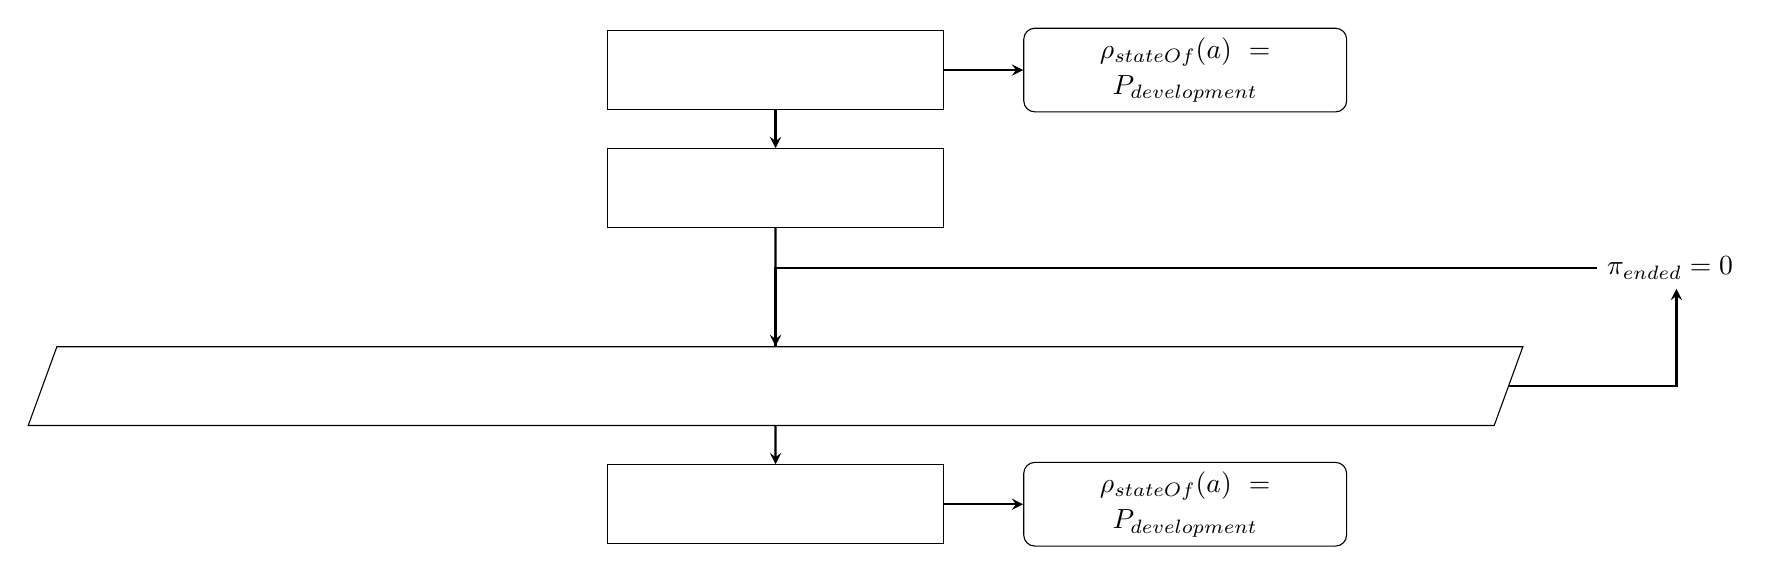
\begin{tikzpicture}[node distance=1.5cm]
\node (LoadByteCode)		[rect, text width=11.5em] 
										{\LoadByteCode};

\node (LoadSourceCode)	[rect, text width=11.5em, below of=LoadByteCode] 
										{\LoadSourceCode};

\node (ValidationEnded)	[event, text width=11.5em, below=1.5cm of LoadSourceCode]
										{\ValidationEnded};
										
\node (aux0)[right=2cm of ValidationEnded]{};
\node (Invalid)					[text width=5em, above of=aux0]
										{$\pi_{ended} = 0$};

\node (ChangeStatus)		[rect, text width=11.5em, below of=ValidationEnded]	
										{\ChangeStatus};

\node (InDevelopment)		[inout, text width=11em, right=1cm of LoadByteCode]			
										{$\rho_{stateOf}(a) = P_{development}$};
										
\node (InProduction)			[inout, text width=11em, right=1cm of ChangeStatus]			
										{$\rho_{stateOf}(a) = P_{development}$};

%arrows
\draw [arrow] (LoadByteCode)				-- (LoadSourceCode);
\draw [arrow] (LoadByteCode)				-- (InDevelopment);
\draw [arrow] (LoadSourceCode) 			-- (ValidationEnded);
\draw [arrow] (ValidationEnded)			-- (ChangeStatus);
\draw [arrow] (ValidationEnded)			-| (Invalid);
\draw [thick]  (Invalid)  							-| (ValidationEnded);
\draw [arrow] (ChangeStatus)				-- (InProduction);

\end{tikzpicture} 
\end{center}

\subsubsection{Ballot smart contract}
\label{tech-apps-voting-ballot}
%\begin{multicols}{2}
An abstract smart contract describing the requirements for final implementation of voting offers.

\code{address votingToken} – ($\pi_{token}$)\hfill\null\linebreak
A voting-associated token providing the holder with the voting right.

\code{function vote(bool)} – ($\pi_{vote}$)\hfill\null\linebreak
External method to write the decision requesting the method.

\code{function applyProposal()} – ($\pi_{apply}$)\hfill\null\linebreak
Abstract application method based on the successful voting. It is implemented in child smart contracts.

\code{uint agreeVotesCount} – ($\pi_{agree}$)\hfill\null\linebreak
Number of tokens transferred for accepting the decision.

\code{uint rejectVotesCount} – ($\pi_{reject}$)\hfill\null\linebreak
Number of tokens transferred for rejecting the decision.

\code{uint endTime} – ($\pi_{end}$)\hfill\null\linebreak
Voting ending time.

\code{function isEnded()}  - ($\pi_{ended}$)\hfill\null\linebreak
Returns 1 if voting time is over and 0 in other cases.
\begin{equation}
\pi_{ended} = \begin{cases}
	1, & \text{if } \pi_{end} > \Gamma_{time} \\
	0, & \text{overwise}
\end{cases}
\end{equation}

\code{function voteMajorityRule()} – ($\pi_{rule}$)\hfill\null\linebreak 
\hlc{Result of function} $f(x) = 1/x$ where $x$ is the ratio of "for" votes to total number of votes sufficient for accepting the decision:
\begin{equation}
\pi_{rule} = \begin{cases}
	\infty, & \text{if } x = 0 \\
	\frac{1}{x}, & \text{overwise}
\end{cases}
\end{equation}

\code{function compare()} – ($\pi_{compare}$)\hfill\null\linebreak
Returns 1 if number of votes for accepting the decision complies with voting conditions for accepting the decision.
\begin{equation}
\pi_{compare} = \begin{cases}
	1, & \text{if }\pi_{agree} * \pi_{rule} > \pi_{agree} + \pi_{reject} \\
	0, & \text{overwise}
\end{cases}
\end{equation}

\code{function isSuccess()} – ($\pi_{success}$)\hfill\null\linebreak
Returns 1 if voting is successful and 0 in other cases.
\begin{equation}
\pi_{success} = \begin{cases}
	1, & \text{if } \pi_{ended} \wedge \pi_{compare} \\
	0, & \text{overwise }
\end{cases}
\end{equation}
%\end{multicols}
\subsection{Musical Assets Registry}
\label{tech-apps-assets}
%\begin{multicols}{2}
The application is used to register musical assets on Musereum platform. The DApp consists of:
\begin{enumerate}
	\item \code{MusicalAssetsRegistry} (MAR – $\psi$)\hfill\null\linebreak
	Root	smart contract of the DApp. Performs factory and ledger functions.
	\item \code{AssetContract} – ($\alpha$)\hfill\null\linebreak
	Musical asset smart contracts produced in MAR.
	\item \hyperref[tech-apps-dal]{Decentralized labels} smart-contracts associated with \code{AssetContract}.
	\item \code{AssetRegistryBallot} – ($\pi^{regAsset}$)
	\item \code{AssetUnregistryBallot} – ($\pi^{unregAsset}$)
	\item User Graphical Interface \hfill\null\linebreak
	web-applications within Musereum Wallet
\end{enumerate}
%\end{multicols}
\subsubsection{Smart-contract MusicalAssetsRegistry}
\label{tech-apps-assets-registry}
%\begin{multicols}{2}
Smart contract tasks: Recording registered musical assets, creating musical asset registration requests through voting in \hyperref[tech-apps-voting]{Voting dApp}.

Only system-authorized registrators participate in the voting.

The ledger is fully public and is open for audit by any member of the network.

History data is accessible by creating a contract request for the event log:
%\end{multicols}

\code{event NewAsset(address indexed asset, uint indexed index)} – ($\psi_{NewAsset}$)\hfill\null\linebreak
Returns the musical asset adding event log  to the ledger with assigned index in the ledger.
\textit{The event is triggered at the moment of creating registration request, not at the time of registration.}
\begin{equation}
\psi_{NewAsset} = \mathcal{E}(asset, index), \quad a \in \mathbb{A} \wedge i \in \mathbb{N}
\end{equation}

\code{event RegistryAsset(address indexed asset, uint indexed index)} – ($\psi_{RegistryAsset}$)\hfill\null\linebreak
Returns event log subset $\psi_{NewAsset}$ associated with asset addresses that have been successfully voted for adding to the public ledger.
\begin{equation}
\psi_{RegistryAsset} \subset \psi_{NewAsset}
\end{equation}

\code{event UnregistryAsset(address indexed asset, uint indexed index)} – ($\psi_{UnregistryAsset}$)\hfill\null\linebreak
Returns subset $\psi_{RegistryAsset}$ for musical assets that have been deleted from Musereum public ledger based on the community decision.
\begin{equation}
\psi_{UnregistryAsset} \subset \psi_{RegistryAsset} \subset \psi_{NewAsset}
\end{equation}

\code{mapping (address => uint) assets} – ($\psi_{assets}(a)$)\hfill\null\linebreak
Associated dictionary of musical assets added to the ledger. 
\begin{equation}
\psi_{assets}(a) = \begin{cases}
	i, & \text{if } a \in \mathcal{S}(\psi_{NewAsset}, [{asset}]) \\
	0, & \text{overwise}
\end{cases}, \quad a \in \mathbb{A} \wedge i \in \mathbb{N}_1
\end{equation}

\code{address[] public assetsIndex} – ($\psi_{index}(i)$)\hfill\null\linebreak
The list of all musical assets added to the ledger. Asset index in the list is equal to the associated dictionary index minus 1.
\begin{align}
i &= \psi_{assets}(a), &a \in \mathbb{A} \wedge i \in \mathbb{N} \\
a &= \psi_{index}(i - 1), &\text{if } i > 0
\end{align}

\subsubsection{Smart-contracts AssetContract}
\label{tech-apps-assets-contract}
The blockchain record about registered musical asset. It contains all the data required to identify a musical asset and define the nature of the asset.

\code{string name} – ($\alpha_{name}$)\hfill\null\linebreak
Name associated with the asset

\code{Multihash meta} – ($\alpha_{meta}$)\hfill\null\linebreak
Hash \hlc{of} meta-date associated with the asset (stored in the decentralized storage)
\begin{align}
\alpha_{meta} &= \mathcal{O}(hash, hashFunction, size), &\alpha_{meta}[hash] &\in \mathbb{B}_{32} \ \wedge \\ 
&&\alpha_{meta}[hashFunction] &\in \mathbb{B} \ \wedge \\
&& \alpha_{meta}[size] &\in \mathbb{B}
\end{align}

\code{event SetAssetType(uint8 indexed typeId)} – ($\alpha_{SetAssetType}$)\hfill\null\linebreak
Returns the asset defining event log containing asset type listing index (\code{AssetTypes} – $\alpha^{types}$).
\begin{equation}
\alpha^{types} \in \mathbb{B}
\end{equation}
\begin{equation}
\alpha_{SetAssetType} = \mathcal{E}(typeId), \quad i \in \alpha^{types}
\end{equation}

\code{mapping (uint8 => bool) type} – ($\alpha_{type}(i)$)\hfill\null\linebreak
Associated dictionary of asset types.
\begin{equation}
\alpha_{type}(i) = \begin{cases}
1, & \text{if } i \in \alpha_{SetAssetType} \\
0, & \text{overwise}
\end{cases}, \quad i \in \alpha^{types}
\end{equation}

\subsubsection{AssetRegistryBallot smart contract}
\label{tech-apps-assets-regballot}
Implementation of \code{Ballot} smart-contract to vote for accepting assets in Musereum ledger.

\subsubsection{AssetUnregistryBallot smart contract}
\label{tech-apps-assets-unregballot}
Implementation of \code{Ballot} smart-contract to vote for excluding assets from Musereum ledger.

\subsection{Decentralized Autonomous Labels}
\label{tech-apps-dal}
%\begin{multicols}{2}
Decentralized autonomous label is a governing smart contract with associated musical asset. DAL is able to:
\begin{enumerate}
	\item Define the label charter that regulates decision making rules;
	\item Issue and sell licenses for commercial use of associated musical asset;
	\item Accumulate and distribute musical asset income,
	\item Distribution and recording the rights for a musical asset with a digital proof-token.
\end{enumerate}

The musical asset is managed on the basis of a token holder democratic voting.

DAL capabilities are implemented with the set of smart contracts:
\begin{itemize}
	\item\code{DALRegistry} – ($\delta^R$)\hfill\null\linebreak
	The ledger of registered decentralized autonomous labels
	\item\code{DALContract} – ($\delta$)\hfill\null\linebreak
	Smart-contract of a decentralized autonomous label
	\item\code{DALToken} – ($\tau^\delta$)\hfill\null\linebreak
	Smart-contract of a token proving the holder's right to participate in a decentralized label
	\item \hlc{Set of voting smart-contracts} for \code{Ballot} implementation:
	\begin{itemize}
		\item\code{CharterChangeVotingRulesBallot}
		Voting offer to change voting rules and make changes to the charter
		\item\code{CharterChangeProposalBallot}\hfill\null\linebreak
		Offer to make changes to the charter
		\item\code{AddLicenseBallot}\hfill\null\linebreak
		Offer to create a new license
		\item\code{CloseLicenseBallot}\hfill\null\linebreak
		Offer to stop selling the license
		\item\code{ReplaceLicenseBallot}\hfill\null\linebreak
		Offer to replace/make changes to the license
	\end{itemize}
\item\code{DALAssetLicense} – ($\theta$)\hfill\null\linebreak
License smart contract for commercial use
\item\code{DALAssetLicenseRule} – ($\theta'$)\hfill\null\linebreak
License-derived smart contract to limit the use 
\end{itemize}
%\end{multicols}
%\vfill\null\pagebreak
\subsubsection{DALRegistry smart contract}
\label{tech-apps-dal-registry}
The ledger of registered autonomous labels is required to keep record and provide access to the label for the manager of associated musical asset.

\code{mapping (address => address) assetLabels} – ($\delta^R_{labels}(a)$)\hfill\null\linebreak
Associated dictionary of created decentralized labels.

\code{event CreateLabel(address indexed asset,}\hfill\null\linebreak
\code{~~~~~~~~~~~~~~~~~~address indexed label,}\hfill\null\linebreak
\code{~~~~~~~~~~~~~~~~~~uint indexed index)~~~} – ($\delta^R_{CreateLabel}$)\hfill\null\linebreak
Returns set of decentralized label creation events. The event consists of: Address of created label, address of associated musical asset and assigned ledger index of the label.
\begin{equation}
\begin{aligned}
\delta^R_{CreateLabel} \in \mathcal{E}(asset, label, index)
asset \in \mathcal{S}(\psi_{RegistryAsset}, [asset]) \subset \mathbb{A}^\alpha \ \wedge \\
label \in \mathbb{A}^\delta \ \wedge \\
index \in \mathbb{N}_1
\end{aligned}
\end{equation}
\code{event CreateLabelBallot(address indexed label,~} \hfill\null\linebreak
\code{~~~~~~~~~~~~~~~~~~~~~~~~address indexed ballot)} – ($\delta^R_{CreateLabelBallot}$)\hfill\null\linebreak
Returns set of decentralized label voting creation events.

The event consists of: Addresses of decentralized label and addresses of created voting.
\begin{equation}
\begin{aligned}
\delta^R_{CreateLabelBallot} \in \mathcal{E}[label, ballot] \\
label \in \mathcal{S}(\delta^R_{CreateLabel}, [label]) \subset \mathbb{A}^\delta \ \wedge \\
ballot \in \mathcal{S}(\phi_{CreatedBallot}, [ballot]) \subset \mathbb{A}^\pi
\end{aligned}
\end{equation}
\code{event FinishLabelVoting(address indexed label,~}\hfill\null\linebreak
\code{~~~~~~~~~~~~~~~~~~~~~~~~address indexed ballot,}\hfill\null\linebreak
\code{~~~~~~~~~~~~~~~~~~~~~~~~bool indexed result)~~~} – ($\delta^R_{FinishLabelVoting}$)\hfill\null\linebreak
Returns subset  $\delta^R_{CreateBallot}$ for complete	d voting with clear indication of success or failure of the offer.

\begin{equation}
\begin{aligned}
f_Z(\mathbb{E}') = \{\mathbb{E}'_i : \ \forall \ \mathbb{E}'_i[ballot][ended] > 0 \} \\
\delta^R_{FinishLabelVoting} = f_Z(\delta^R_{CreateLabelBallot}) \\
\end{aligned}
\end{equation}

\code{event NewLabelLicense(address indexed label, address indexed license)} – ($\delta^R_{NewLicense}$)\hfill\null\linebreak
Returns set of events created by license decentralized label.

\code{event RemoveLabelLicense(address indexed label, address indexed license)} – ($\delta^R_{RemoveLicense}$)\hfill\null\linebreak
Returns subset $\delta^R_{NewLicense}$ for licenses removed from sale.

\subsubsection{DALContract smart contract}
\label{tech-apps-dal-label}
%\begin{multicols}{2}
Smart contract for managing musical asset. Asset and associated entities are managed through proposing an offer for voting with preliminary distribution of \code{VotingRightsToken}among all community participants based on the balance of associated \code{DALToken}.
 
Decentralized label is created automatically based on the registration of the associated asset in the ledger \code{MusicalAssetsRegistry}.

1,000,000,000 proof-tokens are issued upon creation of a decentralized label; at that, in order to simplify the calculations the actual number in associated user interfaces is divided by $10^7$. 

Thus, sole label ownership is equal to 100.0000000 tokens, the minimal vote in the company is 0.0000001\%.

\code{DALToken} holders' rights::
\begin{enumerate}
	\item Participating in royalty distribution
	\item Participating in voting for offers
	\item Cession of tokens to other platform participants by exchanging for ETM or other tokens
\end{enumerate}
%\end{multicols}
\subsubsection{DALToken smart contract}
\label{tech-apps-dal-token}
%\begin{multicols}{2}
Decentralized label token is a \hyperref[tech-blockchain-contracts]{ERC-20} compatible token.

Required changes are added to standard ERC-20 token code to provide operation of distribution system:
\begin{enumerate}
	\item One-to-one link with associated label in \code{label} field is maintained
	\item \code{withdrawRevenueFor()} calls in \code{transfer(...)} и \code{transferFrom(...)} functions for sender and receiver are introduced to \hyperref[tech-apps-dal-royalty-optimization]{improve distribution algorithm}
	\item \code{makeVoteToken()} method is implemented to create \code{VotingRightsToken} associated with current balances
\end{enumerate}
%\end{multicols}
\subsubsection{Royalty distribution}
\label{tech-apps-dal-royalty}
%\begin{multicols}{2}
Royalty is ETM units received on the balance of linked decentralized autonomous label upon commercial activity of associated musical asset.

Every label participant can implement the right to receive royalty share at any moment of time according to the current amount of tokens.
%\end{multicols}
\begin{equation}
\def\arraystretch{1.3}
\begin{array}{@{}llll@{}}
\toprule
    & \multicolumn{2}{c@{}}{\text{Royalty distribution}} & \\
\cmidrule(l){2-3}
    & a = T_{from} & \text{Initial withdrawal transaction} & \\
    & d = \delta(T_{to}) & \text{DAL instance} & \\
    & r = \tau^\delta(d_{token}) & \text{Rights tokens of corresponding DAL} & \\
    & h = \mathbb{K}_n & \text{Height of latest block} & \\
    & b_h = r_{balanceOf}(a) & \text{Balance of DAL rights tokens at block } h & \\
    & t_h = r_{totalSupply} & \text{Total supply of rights token (typically is } 10^9 \text{)} & \\
    & s_h = \frac{b_h}{t_h} & \text{Stake of } a \text{ at moment } h & \\
    & I_h = x & I_h \text{ income of a DAL at moment } h & \\
    & T_h = \sum\limits^{h}_{i=1} I_i & \text{Total lifetime income of DAL} & \\
    & W_h = s * (T_h - \sum\limits^{h-1}_{i=1} W_i) & \text{Available withdrawal amount at moment } h & \\
\bottomrule
\end{array}
\end{equation}
\subsubsection{Distribution algorithm optimization}
\label{tech-apps-dal-royalty-optimization}
%\begin{multicols}{2}
An additional associated list  \code{incomeAtLatestWithdraw(address => uint)} keeping the value at the moment of the latest fund withdrawal for associated address is introduced in the smart contract  to optimize it and avoid calculating $W_h$ for every unique $h$.

This method allows to calculate royalty only when it is required by business logic and only for associated holders.

If rights are transferred to a third party (token transfer), it triggers automatic calculation algorithm of available royalty for the current and the future holder.
%\end{multicols}
%\subsubsection{Голосование за принятие решений}
%\label{tech-apps-dal-voting}
%\subsubsection{Устал децентрализованного лейбла}
%\label{tech-apps-dal-charter}
\subsubsection{DALAssetLicense smart contract}
\label{tech-apps-dal-license}
%\begin{multicols}{2}
%Лицензии на базе смарт-контрактов привязываются к токенам трека и определяют характер использования композиции и ценовую политику, включая различные ценовые настройки в зависимости от географии использования. Коммерческие лицензии обладают сроком действия, задаваемым администратором. Перевыпуск лицензии по окончанию срока создается автоматически с теми же параметрами и отправляется запрос/уведомление акционерам трека. Если акционеры в течение определенного периода выразили свое несогласие, то администратор перевыпускает лицензии с другими параметрами. Консенсус достигается при согласии 51% держателей токенов на трек. Смарт-лицензия состоит из четырех элементов: юридического и простого текста, кода смарт-контракта, механизма API для чтения метаданных и встраивания продаж на сторонние платформы. Смарт-лицензии распределяют роялти между держателями токенов трека. 

Musereum licensing has the capability to conduct the following types of licensing.

Sale of license for commercial use of associated musical asset is the primary task of a decentralized label, at that receiving royalty is the basic motivation for existence.

All licenses are issued as \hlc{an instance} of \code{DALAssetLicense} smart-contract through \code{DALContract} management interface.
The task of \code{DALAssetLicense} root contract is to define the nature of license, acquisition rules and  limitations of use. \code{DALAssetLicense} is a container that provides holder with an unlimited license for commercial use, at that limitations are described in derivative smart contracts:
 \code{DALAssetLicenseRule}.

%\end{multicols}
\paragraph{DALAssetLicenseRule}\hfill\null\linebreak
%\begin{multicols}{2}
It is an abstract smart contract defining the limitation of a parental license; there are 7 basic types of limitations:
\begin{enumerate}
	\item \code{EnumerateRule} – enumerate limitation
	\item \code{RangeRule} – range limitation
	\item \code{ValueRule} – value limitation
	\item \code{AddressRule} – address(es) limitation
	\item \code{TextRule} – descriptive limitation
	\item \code{AllOfRule} – grouping limitation according to type: all from the group
	\item \code{AnyOfRule} – grouping limitation according to type: any from the group
\end{enumerate}

Final limitation can be selected from ready options or it can be created by a decentralized label for a certain license.
%\end{multicols}

\textbf{Rules compare}
\begin{equation}
\begin{aligned}
a = \theta'(original), \quad b = \theta'(target) \\
\theta'_{fitWith}(b) = \begin{cases}
	1, & \text{if } a_{type} = b_{type} \ \wedge \ f_z(a, b) \\
	0, & \text{overwise}
\end{cases}
\end{aligned}
\end{equation}
\code{EnumerateRule}
\begin{equation}
f_z(a, b) = \begin{cases}
	a_{items} \subset b_{items}, & \text{if } a_{all} \\
	|\{i: \forall \ a_{items}[i] \in b_{items}\}|> 0, & \text{overwise}
\end{cases}
\end{equation}
\code{RangeRule}
\begin{equation}
\begin{aligned}
f_z(a, b) = a_{min} > b_{min} \ \wedge \ b_{max} > a_{max}
\end{aligned}
\end{equation}
\code{ValueRule}
\begin{equation}
\begin{aligned}
f_z(a, b) = \begin{cases}
	a_{value} = b_{value}, & \text{if } a_{equal} \\
	a_{value} < b_{value}, & \text{if } a_{less} \\
	a_{value} > b_{value}, & \text{if } a_{more}
\end{cases}
\end{aligned}
\end{equation}
\code{AddressRule}
\begin{equation}
f_z(a, b) = a_{addresses} \in b_{addresses}
\end{equation}
\code{AllOfRule}
\begin{equation}
f_z(a, b) = ||\{\top: a_{items}[i]_{fitWith}(b) = \top\}|| = ||a||
\end{equation}
\code{AnyOfRule}
\begin{equation}
f_z(a, b) = ||\{\top: a_{items}[i]_{fitWith}(b) = \top\}|| > 0
\end{equation}


\begin{table}[H]
\centering
\caption{Types of Rules}
\begin{tabular}{p{0.2\linewidth}p{0.65\linewidth}cc}
\toprule
Code Name & Description \\
\bottomrule
\toprule
\multicolumn{2}{c}{\code{EnumerateRule}} \\
\midrule
	\code{LocationRule} & Geographical use limitation and derivatives: \code{CountryRule} and \code{CityRule} \\
	\code{ChannelRule} & Playback channel limitation \\
	\code{MediaRule} & Media type limitation \\
	\code{GenreRule} & Media genre limitation (used for cinemas, theatres etc.) \\
	\code{UsageRule} & Usage type limitation \\
\bottomrule
\toprule
\multicolumn{2}{c}{\code{RangeRule}} \\
\midrule
	\code{PlayTimesRule} & Playback quantity/period limitation \\
	\code{LifetimeRule} & Validity of license limitation \\
	\code{NumberOfCopyRule} & Number of copies limitation \\
	\code{PowerOfRule} & Project budget and (or) buyer income limitation \\
\bottomrule
\toprule
\multicolumn{2}{c}{\code{ValueRule}} \\
\midrule
	\code{PriceRule} & License price \\
\bottomrule
\end{tabular}
\end{table}

%\subsubsection{Устав децентрализованного лейбла}
%\label{tech-apps-dal-charter}
%\subsection{Fundraising dApp}
%\label{tech-apps-fundraising}
%\begin{multicols}{2}
%Любой \hyperref[tech-apps-dal]{децентрализованный лейбл} 
%\end{multicols}
\subsection{Soundchain}
\label{tech-apps-soundchain}
%\begin{multicols}{2}
Soundchain is the first project that aims to embrace Musereum Foundation. The primary application of Soundchain is to allocate royalty to decentralized labels for listening to musical assets.

Soundchain operation is determined by numerous smart-contracts and interaction interfaces, 
consider PayPerPlay smart-contract that is used to:
\begin{itemize}
	\item record every listening to a musical asset;
	\item generate the royalty payment list from selected Musereum Foundation Volume
\end{itemize}
%\end{multicols}
\begin{align}
& \text {Let } n \text{ is a moment of time and} \nonumber\\
& \text{Let } r \text{ is a money available to pay-per-play for} \nonumber\\
& \text{Set of plays } a \text{ , where } a_i \text{ is a tuple:}  \nonumber\\
a = &\{a_i \ | \ \forall i \in a, a_i \equiv \mathcal{O}[listener, asset, times, sign] \} \\
b = &\{b_i \ | \ \forall i \in a, b_i = f_{pay}(a_i), b_i \in (0; 1) \} \\ 
c = &\sum\limits^{|b|}_{i=0} b_i, \quad d = \frac{r}{c} \\
& \nonumber\\
& \text{Finaly } p \text{ is a set of payments: } \nonumber\\
p = &\{ p_i \ | \ \forall i \in b, p_i = d * b_i \}, \quad r = \sum\limits^{|p|}_{i=0} p_i
\end{align}

Now we need to define what is $f_{pay}$ function. The function result depends on two variables: Listener ratio and label ratio:
\begin{align}
f_{pay}(a) = min(&f_{listenerCoef}(a)),\\
						 &f_{labelCoef}(\delta^{R}_{labels}(a_{asset}))
\end{align}

Listener ratio determines how much trust the platform puts in the listener: 
\begin{enumerate}
	\item Account personification: Full name, location;
	\item Phone number confirmation (Proof-of-SMS);
	\item Geographical location confirmation: verification of documents;
	\item The amount of financial incentive in the future of the platform: Amount of ETMs, amount of held tokens of a decentralized organizations.
\end{enumerate}

When calculating, label ratio takes into account:
\begin{enumerate}
	\item License sale total revenue of associated asset;
	\item License sale revenue for the latest week;
	\item Soundchain artificial label evaluation ratio (additional depositing, fund burning etc.)
\end{enumerate}
\begin{equation}
\end{equation}


%\subsection{Decentralized Marketplace}
%\label{tech-apps-marketplace}
%\end{multicols}

\chapter{Token Sale}
\label{tokensale}

\section{Rationale for token sale}
\label{tokensale-rationale}
Our final goal is to develop a tamper-proof decentralized platform allowing for trustless interactions between major industry players. The project aims to facilitate the transformation of the music industry and introduce modern solutions to deal with the traditional problems.
 
We believe that turning to the traditional schemes of raising capital may not be beneficial to the project in the long run, because it may create an unnecessary conflict of interests between investors controlling the raised funds and the goals of the project.
 
That is why we have decided to conduct a pre-sale of ETM tokens, so that we can provide the access to the value generated by our platforms to those who can use it to the fullest extent – we believe that industry players, who will be the main users and beneficiaries of our platform, will also be the main buyers of our tokens during pre-sale. That way we can not only acquire the necessary financing to develop our project, but will be also able to assess the needs of our participants and better understand the priorities during the development stage. To some extent token sale could be considered as a part of marketing research with the economic incentive for the participants to provide the sincerest answers - they are voting with their stake.


\begin{table}[H]
\centering
\caption{Token Distribution}
\vspace{20pt}
\begin{tabular}{p{0.23\linewidth}p{0.65\linewidth}}
\toprule
\multicolumn{2}{c}{Distribution of tokens} \\
\bottomrule
\midrule
\texttt{250,000,000} & 
Total number of ETM tokens generated with
 the launch of the platform \\
\midrule
\texttt{25,000,000} & 
Number of ETM tokens generated annually, of which 70\% are used to subsidize Soundchain Pay-per-Play contracts \\
\midrule
\texttt{10,000,000} &
Number of ETM tokens to be sold in 2017 at the pre-sale at the 50000 ETM per BTC price \\
\midrule
\texttt{25,000,000} & 
Number of ETM tokens distributed among team members and frozen for 18 months after the launch of the platform \\
\midrule
\texttt{15,000,000} &
Number of ETM tokens distributed among the advisors, bounty and bug bounty hunters \\
\midrule
\texttt{100,000,000} &
Number of ETM tokens to be sold in 2018 at the first public sale with the price to be announced later \\
\midrule
\texttt{100,000,000} &
Number of ETM tokens to be frozen until 2020 and then sold at the second public sale via the auction \\
\bottomrule
\end{tabular}
\end{table}


\chapter{Risks}
%\begin{multicols}{2}
\label{risks}

Acquisition of ETM tokens involves a high degree of risk. Each potential purchaser of ETM tokens should carefully consider the following information about these risks before deciding to purchase ETM tokens. Any of the following risks may adversely affect the platform and the value of the ETM tokens.

Risks and uncertainties described below may not be the only token holders experience. Additional risks and uncertainties may also adversely affect the Platform or the value of the ETM tokens.

Since ETM tokens are not intended to be used as an investment instrument, we strongly recommend to not purchase ETM tokens for purposes other than using the Platform services. 

\section{Risks connected to the value of ETM tokens}
\label{risks-value}

\subsection*{Lack of Development of Market for ETM tokens}
\label{risks-value-lack}
Because there has been no prior public trading market for the ETM Tokens, the Token sale may not result in an active or liquid market for the ETM Tokens, and their price may be highly volatile.

Even if the ETM Tokens are tradable in a secondary market, in practice, there may not be enough active buyers and sellers or the bid-ask spreads may be too wide. The Token holders may not be able to exit their token holdings easily. In the worst-case scenario where no secondary market develops, a Token holder may not be able to liquidate his/her token holdings at all. The exchanges or platforms that facilitate secondary trading of the Tokens may not be regulated by the applicable laws.

\subsection*{Risks Relating to Highly Speculative Traded Price}
\label{risks-value-speculative}
The valuation of digital tokens in a secondary market is usually not transparent, and highly speculative. The Tokens do not hold any ownership rights to Musereum assets and, therefore, are not backed by any tangible asset. Traded price of the ETM Tokens can fluctuate greatly within a short period of time. There is a high risk that a Token holder could lose the entire contribution amount. In the worst-case scenario, the Tokens could be rendered worthless.

\subsection*{ETM Tokens May Have No Value}
\label{risks-value-no-value}
The ETM tokens may have no value and there is no guarantee or representation of liquidity for the ETM tokens. Musereum is not and shall not be responsible for or liable for the market value of the ETM tokens, the transferability and/or liquidity of the ETM tokens and/or the availability of any market for the ETM tokens through third parties or otherwise.

\subsection*{Tokens are Non-Refundable}
\label{risks-value-non-refundable}
Musereum is not obliged to provide the Token holders with a refund related to the Tokens for any reason, and the Token holders will not receive money or other compensation in lieu of the refund. No promises of future performance or price are or will be made in respect to the ETM Tokens, including no promise of inherent value, no promise of continuing payments, and no guarantee that the ETM Tokens will hold any particular value. 

\section{Blockchain and software risks}
\label{risks-block}

\subsection*{Blockchain Delay Risk}
\label{risks-block-delay}
On the Bitcoin and Ethereum blockchains, timing of block production is determined by proof of work so block production can occur at random times. For example, the Cryptocurrency transferred in the final seconds of a distribution period during the Token Sale may not get included for that period. Bitcoin or Ethereum blockchain may not include the transaction within the expected time, in the worst case scenario making the participation in the Token sale impossible.

\subsection*{Blockchain Congestion Risk}
\label{risks-block-congestion}
The Bitcoin and Ethereum blockchains are prone to periodic congestion during which transactions can be delayed or lost. Individuals may also intentionally spam the respective network in an attempt to gain an advantage in purchasing cryptographic tokens. It means that Bitcoin or Ethereum block producers may not include the transaction or include it at all.

\subsection*{\hlc{Risk of Software Weaknesses}}
\label{risks-block-weaknesses}
The concept of smart contract which creates the mechanism of creation and distribution of the ETM tokens, the underlying software application and software platform (i.e. the Ethereum blockchain) are still in an early development stage and unproven. There is no representation and warranty that the process for creating the ETM tokens will be uninterrupted or error-free. There is an inherent risk that the software could contain weaknesses, vulnerabilities or bugs causing, inter alia, the complete loss of the cryptocurrency and/or the ETM tokens.

\subsection*{Risk of New Technology}
The Platform, the ETM Tokens and all of the matters set forth in this White Paper are new and untested. The Platform and the ETM Tokens might not be capable of completion, creation, implementation or adoption. The Platform, or the ability to receive tokens associated with the Platform in the future should not be relied on. Even if the Platform is completed, implemented and adopted, it might not function as intended, and any Tokens may not have functionality that is desirable or valuable. Also, technology is changing rapidly, so the Platform and the ETM Tokens may become outdated.

\section{Security Risks}

\subsection*{Risk of Loss of Private Keys}
The ETM Tokens purchased may be held in a digital wallet or vault, which requires a private key, or a combination of private keys, for access. Accordingly, loss of requisite private keys associated with such will result in loss of such Tokens, access to ETM Token balance and/or any initial balances in blockchains created by third parties. Moreover, any third party that gains access to such private keys, including by gaining access to login credentials of a hosted wallet or vault service used, may be able to misappropriate the ETM Tokens. Musereum is not responsible for any such losses.

\subsection*{Lack of ETM Token Security}
The ETM Tokens may be subject to expropriation and or/theft. Hackers or other malicious groups or organizations may attempt to interfere with the Platform or the ETM Tokens in a variety of ways, including, but not limited to, malware attacks, denial of service attacks, consensus-based attacks, Sybil attacks, smurfing and spoofing. Furthermore, there is the risk that our smart contracts may contain intentional or unintentional bugs or weaknesses which may negatively affect the Tokens or result in the loss of Tokens, the loss of ability to access or control the Tokens. In the event of such a software bug or weakness, there may be no remedy and holders of the Tokens are not guaranteed any remedy, refund or compensation.

\subsection*{Risk of Ethereum Mining Attacks}
The blockchain system may be susceptible to mining attacks, including double-spend attacks, majority mining power attacks, “selfish-mining” attacks, and race condition attacks. Any successful attacks present a risk to expected proper execution and sequencing of the Token transactions, and expected proper execution and sequencing of contract computations.

\subsection*{Failure to Map a Public Key to Buyer’s Account}
The wallet or wallet service provider used for the acquisition and storage of the ETM tokens has to be technically compatible with the ETM tokens. The failure to assure this may result in not being able to access ETM tokens.

\subsection*{Risk of Incompatible Wallet Service}
The wallet or wallet service provider used for the acquisition and storage of the ETM tokens has to be technically compatible with the ETM tokens. The failure to assure this may result in not being able to access ETM tokens.

\section{Risks relating to network development}
\subsection*{Risk Related to Reliance on Third Parties}
Even if completed, the Platform will rely, in whole or partly, on third parties to adopt and implement it and to continue to develop, supply, and otherwise support it. There is no assurance or guarantee that those third parties will complete their work, properly carry out their obligations, or otherwise meet anyone’s needs, all of these might have an adverse effect on the Platform.

\subsection*{Dependence of Musereum on Senior Management Team}
The ability of the Musereum project team which is responsible for maintaining competitive position of the Platform is dependent to a large degree on the services of a respective senior management team. The loss or diminution in the services of members of respective senior management team or an inability to attract, retain and maintain additional senior management personnel could have an adverse effect on the Platform. Competition for personnel with relevant expertise is intense due to the small number of qualified individuals, and this situation seriously affects the ability to retain its existing senior management and attract additional qualified senior management personnel, which could have a significant adverse impact on the Platform.

\subsection*{Dependence of Musereum Platform on Various Factors}
The development of the Platform may be abandoned for a number of reasons, including lack of interest from the public, lack of funding, lack of commercial success or prospects, or departure of key personnel.

\subsection*{Lack of Interest to the Musereum Platform}
Even if the Platform is finished and adopted and launched, the ongoing success of the Platform relies on the interest and participation of third parties like developers. There can be no assurance or guarantee that there will be sufficient interest or participation in the Platform.

\subsection*{Changes to the Musereum Platform}
The Platform is still under development and may undergo significant changes over time. Although Musereum intend for the Platform to have the features and specifications set forth in this White Paper, changes to such features and specifications can be made for any number of reasons, any of which may mean that the Platform does not meet expectations.

\subsection*{Risk associated with Other Applications}
The Platform may give rise to other, alternative projects, promoted by unaffiliated third parties, under which the ETM Token will have no intrinsic value.

\subsection*{Risk of an Unfavorable Fluctuation of Cryptocurrency Value}
The proceeds of the sale of the ETM Tokens will be denominated in cryptocurrency, and may be converted into other cryptographic and fiat currencies. If the value of cryptocurrencies fluctuates unfavourably during or after the Token Sale, Musereum may not be able to fund development, or may not be able to develop or maintain the Platform in the manner that it intended.

\section{Risks arising in course of company parties' business}
\subsection*{Risk of Conflicts of Interest}
Musereum may be engaged in transactions with related parties, including respective majority shareholder, companies controlled by him or in which he owns an interest, and other affiliates, and may continue to do so in the future. Conflicts of interest may arise between Musereum affiliates and Musereum, potentially resulting in the conclusion of transactions on terms not determined by market forces.

\subsection*{Risks Related to Invalidation of Company Parties Transactions}
Musereum have taken a variety of actions relating to its business that, if successfully challenged for not complying with applicable legal requirements, could be invalidated or could result in the imposition of liabilities on Musereum. Since applicable legislation may subject to many different interpretations, Musereum may not be able to successfully defend any challenge brought against such transactions, and the invalidation of any such transactions or imposition of any such liability may, individually or in the aggregate, have an adverse effect on the Platform.

\subsection*{Risk Arising from Emerging Markets}
Musereum may operate on emerging markets. Emerging markets are subject to greater risks than more developed markets, including significant legal, economic and political risks. Emerging markets are subject to greater risk than more developed markets, including in some cases significant legal, economic and political risks. Emerging economies are subject to rapid change and that the information set out in this White Paper may become outdated relatively quickly.

\section{Govermental Risks}
\subsection*{Uncertain Regulatory Framework}
The regulatory status of cryptographic tokens, digital assets, and blockchain technology is unclear or unsettled in many jurisdictions. It is difficult to predict how or whether governmental authorities will regulate such technologies. It is likewise difficult to predict how or whether any governmental authority may make changes to existing laws, regulations and/or rules that will affect cryptographic tokens, digital assets, blockchain technology and its applications. Such changes could negatively impact the ETM Tokens in various ways, including, for example, through a determination that the tokens are regulated financial instruments that require registration. Musereum may cease the distribution of the tokens, the development of the Platform or cease operations in a jurisdiction in the event that governmental actions make it unlawful or commercially undesirable to continue to do so.

\subsection*{Failure to Obtain, Maintain or Renew Licenses and Permits}
Although as of the date of starting of the Token sale there are no statutory requirements obliging Musereum to receive any licenses and permits necessary for carrying out of its activity, there is the risk that such statutory requirements may be adopted in the future and may relate to Musereum. In this case, Musereum business will depend on the continuing validity of such licenses and permits and its compliance with their terms. Regulatory authorities will exercise considerable discretion in the timing of license issuance and renewal and the monitoring of licensees’ compliance with license terms.

Requirements which may be imposed by these authorities and which may require Musereum to comply with numerous standards, recruit qualified personnel, maintain necessary technical equipment and quality control systems, monitor our operations, maintain appropriate filings and, upon request, submit appropriate information to the licensing authorities, may be costly and time-consuming and may result in delays in the commencement or continuation of operation of the Platform. Further, private individuals and the public at large possess rights to comment on and otherwise engage in the licensing process, including through intervention in courts and political pressure. Accordingly, the licenses Musereum may need may not be issued or renewed, or if issued or renewed, may not be issued or renewed in a timely fashion, or may involve requirements which restrict Musereum ability to conduct its operations or to do so profitably.


\subsection*{Risk of Government Action}
The industry in which Musereum operate is new, and may be subject to heightened oversight and scrutiny, including investigations or enforcement actions. There can be no assurance that governmental authorities will not examine the operations of Musereum and/or pursue enforcement actions against them. All of this may subject Musereum to judgments, settlements, fines or penalties, or cause Musereum to restructure its operations and activities or to cease offering certain products or services, all of which could harm Musereum reputation or lead to higher operational costs, which may, in turn, have an adverse effect on the Tokens and/or the development of the Platform.

\subsection*{Risk of Burdensomeness of Applicable Laws, Regulations and Standards}
Failure to comply with existing laws and regulations or the findings of government inspections or increased governmental regulation of Musereum operations, could result in substantial additional compliance costs or various sanctions, which could adversely affect Musereum business and the Platform. Musereum operations and properties are subject to regulation by various government entities and agencies, in connection with ongoing compliance with existing laws, regulations and standards. Regulatory authorities exercise considerable discretion in matters of enforcement and interpretation of applicable laws, regulations and standards.

Respective authorities have the right to, and frequently do, conduct periodic inspections of Musereum operations and properties throughout the year. Any such future inspections may conclude that Musereum has violated laws, decrees or regulations, and it may be unable to refute such conclusions or remedy the violations.

Musereum failure to comply with existing laws and regulations or the findings of government inspections may result in the imposition of fines or penalties or more severe sanctions or in requirements that respective Musereum cease certain of its business activities, or in criminal and administrative penalties applicable to respective officers. Any such decisions, requirements or sanctions, or any increase in governmental regulation of our operations, could increase Musereum costs and adversely affect Musereum business and the Platform.


\subsection*{Unlawful or Arbitrary Government Action}
Governmental authorities may have a high degree of discretion and, at times, act selectively or arbitrarily, without hearing or prior notice, and sometimes in a manner that is contrary a law or influenced by political or commercial considerations. Moreover, the government also has the power in certain circumstances, by regulation or government act, to interfere with the performance of, nullify or terminate contracts. Unlawful, selective or arbitrary governmental actions have reportedly included the denial or withdrawal of licenses, sudden and unexpected tax audits, criminal prosecutions and civil actions. Federal and local government entities have also used common defects in matters surrounding the Token Sale as pretexts for court claims and other demands to invalidate or to void any related transaction, often for political purposes. In this environment, Musereum competitors may receive preferential treatment from the government, potentially giving them a competitive advantage over Musereum.

%\end{multicols}
\end{document}
